%##################################################################################

\documentclass[12pt,a4paper,twoside]{report}
%\documentclass[12pt,a4paper,oneside]{report}
\usepackage{graphicx}
%\usepackage[ngerman, english]{babel} %-- uncomment this to get english titles
\usepackage[ngerman]{babel}
\usepackage{german,a4}
%\usepackage{picins}
%\usepackage{epsfig}
\usepackage{fancyhdr}			% for nice header and footer
\usepackage{hyperref}			% references in pdf
\usepackage[sf]{titlesec}	%customization of \chapter Titles for appendices
\usepackage{textcomp}
\usepackage{makeidx}
\usepackage{ngerman}			% german Umlauts
\usepackage[utf8]{inputenc}
\usepackage{booktabs}                               % necessary for tabulars
\usepackage[squaren]{SIunits}
\usepackage[numbers,square]{natbib}
\usepackage{amssymb}			% Math symbols
\usepackage{tabto}				% tab spaces
\usepackage{booktabs}			% for tables
\usepackage{multirow}
\usepackage{afterpage} 			% blank page

%\usepackage{wrapfig} 
%\usepackage[pdftex]{graphicx}
%\usepackage{ifthen}  
%\usepackage{booktabs} % fancy tables
%\usepackage[titletoc]{appendix} % custom naming of appendices
\usepackage{amssymb, amsmath, amsthm} % for equations & eqref
%\usepackage{listings} \lstset{basicstyle=\tiny\ttfamily, numbers=left, escapeinside={(*}{*)}, captionpos=b}
%\usepackage{dirtree}

%get bigger \par with one empty line
\newcommand{\mypar}{\par\medskip}

% Command for empty page
\newcommand\blankpage{%
    \null
    \thispagestyle{empty}%
    \addtocounter{page}{-1}%
    \newpage}

%TODO line
\newcommand{\writeTodo}{1}
\newcommand{\todo}[1]{
	\ifdefined \writeTodo
		\mypar\textbf{\textcolor{KITgreen}{TODO: }\textcolor{red}{#1}}\mypar
	\fi
} 
 
%\theoremstyle{plain}% default
\theoremstyle{definition}
\newtheorem{definition}{Definition}

% Abbkürzungsverzeichnis einfügen
%%%%%%%%%%%%%%%%%%%%%%%%%%%%%%%%%%%%%%%%%%%%%%%%%%%%%%%%% 
\usepackage{nomencl}
\let\abbrev\nomenclature
\renewcommand{\nomname}{Abkürzungsverzeichnis}
\setlength{\nomlabelwidth}{.25\hsize}
\renewcommand{\nomlabel}[1]{#1 }%\dotfill}
\setlength{\nomitemsep}{-\parsep}
\makenomenclature
\newcommand{\markup}[1]{\underline{#1}} 

% Farben
\usepackage{color}
\definecolor{KITgreen}{rgb}{0, .61, .51} 
\definecolor{KITbluegrey}{rgb}{.27, .39, .67} 
\definecolor{KITgrey}{rgb}{.49, .49, .49} 

% =====================================================
% Dokumenten-Platzhalter
% =====================================================
% =====================================================
% Dokumenten Platzhalter
% =====================================================


\newcommand{\titelderarbeit}{Bewertung und Vergleich verschiedener Arten faltender künstlicher neuronaler Netze zur Regression der Picklänge kardiovaskulärer Implantate basierend auf Kamerabildern und Deep Learning}
\newcommand{\artderarbeit}{Bachelorarbeit}

\newcommand{\diplomandprefix}{cand. el.}
\newcommand{\diplomand}{Emilio Rivera Cedeño}

\newcommand{\betreuerA}{Benedikt Haas}
\newcommand{\betreuerB}{ }

 
%\newcommand{\nameprefix}{}{}    %use no nameprefix 
\newcommand{\nameprefix}{M. Sc. }
\newcommand{\docauthor}{Benedikt Haas}

\newcommand{\nameprefixb}{}{}    %use no nameprefix 
%\newcommand{\nameprefixb}{Dipl.-Ing.}  
\newcommand{\docauthorb}{}

\newcommand{\nameprefixc}{}{}    %use no nameprefix 
%\newcommand{\nameprefixc}{Dipl.-Ing.}
\newcommand{\docauthorc}{}

%\newcommand{\betreuerA}{nn}
%\newcommand{\betreuerB}{nn}
\newcommand{\abgabe}{30. April 2021}
\newcommand{\versionierungsnr}{v1.0}
\newcommand{\fussnoteninhalt}{}
\newcommand{\leerzeichen}{ }

%% english version
%\newcommand{\Dachorganisation}{Karlsruhe Institute of Technology - KIT}
%\newcommand{\Institut}{Institute for Information Processing 
%												Technology - ITIV}
												
% deutsche version
\newcommand{\Dachorganisation}{Karlsruher Institut für Technologie - KIT}
\newcommand{\Institut}{Institut für Technik der Informationsverarbeitung - ITIV}

% ====================================================
% Formatierung des Dokuments
% ====================================================


%\usepackage{color}
%\usepackage{helvet}

% =====================================================
% Seite einrichten
% =====================================================
\setlength{\textwidth}{160mm} \setlength{\textheight}{235mm}
\setlength{\oddsidemargin}{5mm}
%pagelayout: (1in=25,4mm), default offset of page origin: 1in x 1in
%     25,4+5=30,4mm       160mm          19,6mm
%  |                   sadfasdfasdfasdf          |
\setlength{\evensidemargin}{-5,8mm} 
%     25,4-5,8= 19,6mm    160mm          30,4mm
%  |                   sadfasdfasdfasdf          |
\setlength{\topmargin}{0mm} \setlength{\voffset}{-15mm}
\setlength{\headsep}{12mm} \setlength{\footskip}{15mm}
\setlength{\headheight}{15.5pt}

% =====================================================
% sonstige Einstellungen
% =====================================================
%\flushbottom % Textfluss schoen unten ausrichten
\footnotesep12pt % Abstand Text / Fussnote
%\setlength{\parindent}{0pt} \setlength{\abovecaptionskip}{-6pt}
%\setlength{\belowcaptionskip}{0pt} \setlength{\intextsep}{18pt}
%\renewcommand{\baselinestretch}{1.2} % Zeilenabstand
\setcounter{secnumdepth}{4}
\newcommand{\p}[1]{\texttt{#1}}
\nonfrenchspacing

% =====================================================
% Kopf- und Fusszeile formatieren
% =====================================================
\pagestyle{fancy}
\fancyhead{}
\makeatletter
\if@twoside
	\fancyhead[LO]{\sf{\rightmark}}
	\fancyhead[RE]{\sf{\leftmark}}
	\fancyfoot[LE]{\setlength{\unitlength}{1mm}
		\begin{picture}(0,0) \put(0,-2){
			%
\includegraphics[height=0.6cm,width=0.6cm]{98_images/ITIVlogo.png}
		} \end{picture}
		%\put(9,2){\scriptsize\sf{\Institut}}\put(9,-2){\scriptsize\sf{\Dachorganisation}}}
		\put(0,2){\scriptsize\sf{\Institut}}\put(0,-2){\scriptsize\sf{\Dachorganisation}}}

\else
	\fancyhead[LO]{\sf{\leftmark}}
	\fancyfoot[LO]{\setlength{\unitlength}{1mm} 
		\begin{picture}(0,0) \put(0,-2){
			% 
\includegraphics[height=0.6cm,width=0.6cm]{98_images/ITIVlogo.png}
		} \end{picture}
		%\put(9,2){\scriptsize\sf{\Institut}}\put(9,-2){\scriptsize\sf{\Dachorganisation}}}
		\put(0,2){\scriptsize\sf{\Institut}}\put(0,-2){\scriptsize\sf{\Dachorganisation}}}
\fi
\fancyhead[LE, RO]{\sf{\thepage}}
\makeatother

\cfoot{}
\fancyfoot[RO]{\footnotesize\sf{\titelderarbeit}}
\renewcommand{\headrulewidth}{0.4pt}
\renewcommand{\footrulewidth}{1.0pt}

% ====================================================
% Kopf- und Fusszeile fuer "plain"-Format ueberschreiben
% ====================================================
\makeatletter
\if@twoside
	\fancypagestyle{plain}{%
	\fancyhf{}
	\fancyfoot[LE]{\setlength{\unitlength}{1mm}
		\begin{picture}(0,0) \put(0,-2){
			%
\includegraphics[height=0.6cm,width=0.6cm]{98_images/ITIVlogo.png}
		} \end{picture}
		%\put(9,2){\scriptsize\sf{\Institut}}\put(9,-2){\scriptsize\sf{\Dachorganisation}}}
		\put(0,2){\scriptsize\sf{\Institut}}\put(0,-2){\scriptsize\sf{\Dachorganisation}}}
	\cfoot{}
	\fancyfoot[RO]{\footnotesize\sf{\titelderarbeit}}
	\renewcommand{\headrulewidth}{0pt}
	\renewcommand{\footrulewidth}{1.0pt}}
\else
	\fancypagestyle{plain}{%
	\fancyhf{}
	\fancyfoot[L,C,R]{\setlength{\unitlength}{1mm}
	\begin{picture}(0,0) \put(0,-2){
		%
\includegraphics[height=0.6cm,width=0.6cm]{98_images/ITIVlogo.png}
	} \end{picture}
	%\put(9,2){\scriptsize\sf{\Institut}}\put(9,-2){\scriptsize\sf{\Dachorganisation}}}
	\put(0,2){\scriptsize\sf{\Institut}}\put(0,-2){\scriptsize\sf{\Dachorganisation}}}
	\cfoot{}
	\rfoot{\footnotesize\sf{\titelderarbeit}}
	\renewcommand{\headrulewidth}{0pt}
	\renewcommand{\footrulewidth}{1.0pt}}
\fi

%makes the index do not remove!
\makeindex

\hypersetup{
	%pdftex %schon gesetzt
	pdfauthor = \docauthor,
	%pagebackref,%schon gesetzt
	colorlinks=true,
	linkcolor=black,
	citecolor=black,
	urlcolor=black
	}

\providecommand{\e}[1]{\ensuremath{\times 10^{#1}}}

% =====================================================
% Inhalt der Titelseite definieren
% =====================================================

\makeindex
\newcommand{\Idx}[1]{#1 \index{#1}}

\hyphenation{
EVITA
}

% =====================================================
% Zeichen für Copyright, Trademark, Registerd, ...
% =====================================================
\def\TReg{\textsuperscript{\textregistered}}
\def\TCop{\textsuperscript{\textcopyright}}
\def\TTra{\textsuperscript{\texttrademark}}

% =====================================================
% selbs definierte Zeichen
% =====================================================
\def\zB{z.\,B. }
\def\uvm{u.\,v.\,m.}
\begin{document}

% =====================================================
% Put Titel in English
% ===================================================== 
%
% Inhalt der Titelseite definieren
\pagestyle{empty}
\pagenumbering{roman}
\setcounter{page}{1}

\begin{titlepage}

\begin{minipage}{15cm}
\linespread{1.2}

\begin{tabular}{lr}
\begin{minipage}{0.2\linewidth}

\includegraphics[height=1cm]{98_images/kit.png}
\end{minipage}
&
\begin{minipage}{0.8\linewidth}
\large
%\center
\vspace{7mm}
\begin{flushleft}
\Dachorganisation
\end{flushleft}
\end{minipage}
\\
\\
\begin{minipage}{0.2\linewidth}
\includegraphics[height=1cm]{98_images/ITIVLogo.png}
\end{minipage}
&
\begin{minipage}{0.8\linewidth}
\large
%\center
\vspace{7mm}
\begin{flushleft}
\Institut\\
\end{flushleft}
\end{minipage}
\\
\end{tabular}

\vspace{3cm}

\begin{center}
\Huge
\bfseries  \titelderarbeit
\end{center}

\vspace{1cm}
\begin{center}
\large 
\subtitelderarbeit 
\vspace{1cm}
%\Large
%\textbf{\diplomandprefix\ \diplomand}

\vspace{1cm}
%\Large
%%Berichtsbezeichnung und ID Nummer
 Version 
\versionierungsnr\\
\abgabe%\textbf{\abgabe}
\end{center}
%
\vspace{2.5cm}

\begin{tabular}{rcl}
\bfseries Head of Institute:
&& Prof. Dr.-Ing. J. Becker\\
&& Prof. Dr. rer. nat  W. Stork\\
&& Prof. Dr.-Ing. Eric Sax\\
 \\
	\bfseries Author:         && \nameprefix \leerzeichen \docauthor \\
											      && \nameprefixb \leerzeichen \docauthorb\\
														&& \nameprefixc \leerzeichen \docauthorc \\
											      \end{tabular}											
											      
\end{minipage}
\end{titlepage}
\pagestyle{fancy}
%    \parindent=0pt
%    %\sloppypar
%    \linespread{1.2}
%    \thispagestyle{plain}
%    %\frontmatter
%    %\maketitle

% =====================================================
% Put Titel in Deutsch
% ===================================================== 

% Inhalt der Titelseite definieren
\pagestyle{empty}
\pagenumbering{roman}
\setcounter{page}{1}

\begin{titlepage}

\begin{minipage}{15cm}
\linespread{1.2}

\begin{tabular}{lr}
\begin{minipage}{0.3\linewidth}

\includegraphics[height=2cm]{98_images/kit.png}
\end{minipage}
&
\begin{minipage}{0.7\linewidth}
\large
\center
Karlsruhe Institute of Technology\\
Fakultät für Elektrotechnik
\end{minipage}
\\
\\
\begin{minipage}{0.3\linewidth}
\includegraphics[height=2cm]{98_images/ITIVLogo.png}
\end{minipage}
&
\begin{minipage}{0.7\linewidth}
\large
\center
Institut für Technik der Informationsverarbeitung (ITIV)\\
\end{minipage}
\\
\end{tabular}

% #################################################################
% ### If the Title is very long reduce vspace to less than 2cm
% #################################################################
\vspace{1.5cm}

% #################################################################

\begin{center}
\Huge
\bfseries  \titelderarbeit
\end{center}

\vspace{1cm}
\begin{center}
\large 
\artderarbeit ~von\\
\vspace{1cm}
\Large
\textbf{\diplomandprefix\ \diplomand}

\vspace{1cm}
\Large
\textbf{\abgabe}
\end{center}
%
\vspace{2.5cm}

\begin{tabular}{rcl}
\bfseries Institutsleitung: 
&& Prof. Dr.-Ing. Dr. h.c. J. Becker\\
&& Prof. Dr.-Ing. Eric Sax\\
&& Prof. Dr. rer. nat  W. Stork\\

 \\
	\bfseries Betreuer:       &&\nameprefix  \betreuerA \\
											      && \betreuerB \\
\end{tabular}											
\end{minipage}
\end{titlepage}
    \parindent=0pt
    %\sloppypar
    \linespread{1.2}
    \thispagestyle{plain}
    %\frontmatter
    %\maketitle
    \cleardoublepage
    
% =====================================================
% Abstract
% =====================================================     
	\begin{abstract}
		Die Sicherung der Qualität bei Stents ist von großer Bedeutung sowohl für den Hersteller, als auch für den Patienten. Hierbei ist der Vorgang der visuellen Inspektion aufwendig und fehleranfällig, weshalb der Vorgang automatisiert werden soll, um die Reproduzierbarkeit der Prüfung zu verbessern und ein genaueres Prüfergebnis zu erzielen. Als grundlegende Qualitätsmerkmale gelten in der Geometrie von Stents der Flechtwinkel und die Picklänge.

\mypar In der vorliegenden Arbeit wurden unterschiedliche faltende neuronale Netze implementiert und trainiert, um eine Regression der betrachteten Picklänge im Stent durchzuführen. Diese wurden darauffolgend getestet, sodass die Ergebnisse bewertet und verglichen werden konnten. Hierfür war die Erstellung eines Datensatzes, dessen Erweiterung durch Augmentation und die Vorverarbeitung der Bilddaten notwendig.

\mypar Durch die Evaluation konnte ein neuronales Netz gewonnen werden, das in der Lage ist, die Länge des mittleren Picks eines Bildes mit einer Genauigkeit von 1,764 Pixel oder 0,077 Millimeter innerhalb von 18,9 Millisekunden zu bestimmen. Im Anschluss der Arbeit ist es möglich, eine vereinfachte Form der Fehlerlokalisierung durchzuführen. 

\cleardoublepage

\chapter*{Urheberrecht}

ARM\TReg, AMBA\TReg, AXI\TTra, Cortex\TTra, TrustZone\TTra, SecurCore\TTra  , DSTREAM\TTra und weitere im Text erwähnte ARM-Produkte sowie die entsprechenden Logos sind Marken oder eingetragene Marken der Advanced RISC Machines Ltd.\par
\vspace{0.5cm}
Xilinx\TReg, Zynq\TTra und weitere im Text erwähnte Xilinx-Produkte sowie die entsprechenden Logos sind Marken oder eingetragene Marken der Xilinx Inc.\par
\vspace{0.5cm}
	\end{abstract}
	\cleardoublepage
% =====================================================
% Signaturepage
% ===================================================== 
    \chapter*{}
\begin{flushleft}
\vspace{11cm}
Erklärung\\[1cm]
Ich versichere hiermit, dass ich meine Bachelorarbeit (bzw. Masterarbeit) selbständig und unter Beachtung der Regeln zur Sicherung guter wissenschaftlicher Praxis im Karlsruher Institut für Technologie (KIT) in der aktuellen Fassung angefertigt habe. \\
Ich habe keine anderen als die angegebenen Quellen und Hilfsmittel benutzt und wörtlich oder inhaltlich übernommene Stellen als solche kenntlich gemacht.\\[1cm]

Karlsruhe, den \abgabe\\[1cm]
\end{flushleft}

\begin{center}
---------------------------------\\
\diplomand
\end{center}

	\cleardoublepage
% =====================================================
% TOC
% ===================================================== 
    \tableofcontents
    %\clearpage
    \cleardoublepage

% =====================================================
% Main Chapters
% ===================================================== 
    %\mainmatter
    \pagenumbering{arabic}
    \setcounter{page}{1}
    \pagestyle{fancy}
 \normalsize

    
    \chapter{Einleitung}
    \label{ch:Einleitung}    
    	Nach Angaben des Statistischen Bundesamtes starben in Deutschland im Jahre 2019 195.690 Menschen an einer Herzerkrankung \cite{destatis2}. Dies entspricht etwa ein Fünftel der Sterbefälle in diesem Jahr \cite{destatis}. Um das Risiko eines Herzinfarktes zu reduzieren, werden seit 1988 Stents eingesetzt \cite{sigwart}.

\mypar Stents sind kardiovaskuläre Implantate, welche in Gefäße eingefügt werden, um eine Verstopfung bzw. ein Zusammenfallen derer zu verhindern. Aus diesem Grund muss der Stent gewisse Qualitätsanforderungen erfüllen wie zum Beispiel die geometrischen Verhältnisse dieser Spiralprothesen. Diese werden aktuell stichprobenartig nach der Herstellung durch einen Menschen mittels visueller Inspektion geprüft. Allerdings ist dieser Vorgang zeitaufwendig, für den Inspizierenden anstrengend und daher fehleranfällig. Zudem ist dieser Ablauf in der Produktion  ineffizient, weil der Stent erst nach seiner Fertigung geprüft werden kann.

\mypar Um jeden Stent überprüfen zu können und den möglichen menschlichen Fehler zu beseitigen, soll der Prozess der geometrischen Inspektion automatisiert werden. Eine zur Herstellung parallel geführte Überprüfung nach Defekten würde außerdem das sofortige Ausgleichen von Ungenauigkeiten erlauben. Zudem bietet dieser Ansatz die Möglichkeit, alle Stents zu prüfen. Dementsprechend soll, basierend auf Kamerabildern und Deep Learning, ein effektives System zur Fehlererkennung in Stents entwickelt werden. 


% Zielsetzung
\section{Zielsetzung}\label{sec:zielsetzung-sec}
Ziel dieser Arbeit ist die Überprüfung der Stentgeometrie anhand der Picklängen auf erfassten Kamerabildern. Hierbei soll immer derjenige Pick analysiert werden, der sich in der Bildmitte befindet. Im Spezifischen sollen verschiedene Arten faltender neuronaler Netze evaluiert und anschließend miteinander verglichen werden. Dies schließt eine geeignete Bildvorverarbeitung sowie die Definition geeigneter Vergleichsparameter mit ein. Abschließend soll eine Lokalisierung des Fehlers im Bild möglich sein.


% Aufbau der Arbeit
\section{Aufbau der Arbeit}
Aus diesem Grund setzt sich Kapitel \ref{ch:Grundlagen} mit den für das Verständnis dieser Arbeit notwendigen Grundlagen auseinander. Dazu zählt ein Überblick über Stents, der Histogrammausgleich und der Aufbau und Funktionsweise faltender neuronaler Netze. Darauffolgend wird der aktuelle Stand von Methoden zur Defekterkennung in Stents und Geflechten in Abschnitt \ref{ch:state-of-the-art} vorgestellt. Des Weiteren wird der grundlegende Aufbau des Projektes Stents4Tomorrow \cite{flechtmaschine} in Kapitel \ref{ch:Konzept} dargestellt und die im Rahmen dieser Arbeit relevanten Schritte hervorgehoben. Zudem wird die Berechnung der Picklänge erläutert und die Auswahl der faltenden neuronalen Netze erklärt. Darüber hinaus werden die einzelnen Schritte der Datenvorverarbeitung und Implementierung der neuronalen Netze in Kapitel \ref{ch:implementierung} beschrieben und begründet. Im Übrigen werden die erworbenen Ergebnisse in Abschnitt \ref{ch:Bewertung} bewertet und miteinander verglichen. Hierfür werden diese vorgestellt und ausgewertet, um die faltenden neuronalen Netze anhand festgelegter Vergleichsfaktoren zu vergleichen. Anschließend werden die Ergebnisse in Kapitel \ref{ch:Fazit} zusammengefasst und die nächsten Schritte im Sinne eines Ausblicks erläutert.




    \cleardoublepage
    
    \chapter{Grundlagen}
    \label{ch:Grundlagen}
		% Einleitung
Dieses Kapitel stellt die grundlegenden Konzepte über Stents und faltende neuronale Netze vor, die für ein Verständnis dieser Arbeit benötigt werden. Der erste Unterabschnitt beginnt mit einer Einführung zu Stents und deren Einsatzgebiete in der Medizin. Des Weiteren wird das Herstellungsverfahren und die Geometrie des Aufbaus eines Stents erläutert. 

\mypar Das Kapitel beginnt mit einen kurzen Einblick in einige Verfahren des Histogrammausgleichs aus der Bildverarbeitung und wird mit den Grundlagen zu faltenden neuronalen Netzen fortgeführt. Hierbei wird sowohl in die Bausteine, als auch in die daraus bestehenden Netzwerkarchitekturen eingegangen. Zudem wird der Vorgang des Trainings eines neuronalen Netzes konkretisiert. 


% 2.1 Stents
\section{Stents}\label{sec:?}
Am 12. Juni 1986 veränderten Ulrich Sigwart und Jacques Puel, mit der ersten Anwendung eines Stents bei Menschen, die Behandlung der ischämischen Herzkrankheit. Es handelte sich um ein selbstexpandierendes geflochtenes Gittergewebe aus 16 Drähten mit einen Durchmesser von 60 $\mu$m. Wie in Abbildung \ref{fig:stent_view} zu sehen ist, war der Stent an einen Abgabekatheter durch eine einziehbare Plastikmembran gebunden. \cite{sigwart}

\begin{figure}[h!]
\centering
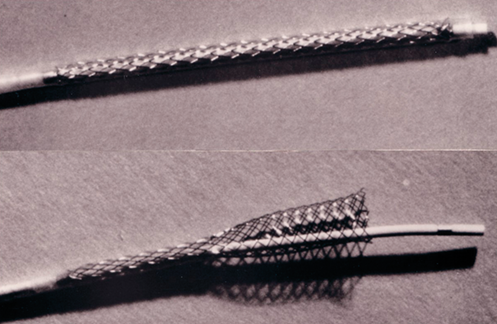
\includegraphics[width=9cm]{98_images/first_stent.png}
\caption{Der erste selbstexpandierbare Stent. Oben am Abgabekatheter gebunden. Unten zum Teil bereitgestellt durch Zurückziehen der Membran \cite{sigwart}.}
\label{fig:stent_view}
\end{figure}

\mypar Diese Art von Prothesen dienen als Instrument zum Offenhalten von Gefäßen oder Hohlorganen. Meistens bestehen diese aus Kunststoffen oder Metallen. Stents stabilisieren verengte Gefäße durch das Erweitern dieser und vermeiden einen erneuten Verschluss oder eine Verengung. Die Oberfläche des Gefäßes wird geglättet und Ablagerungen werden vom Stent gegen die Innenwand gepresst. Dies führt zu einer Verbesserung des Blutflusses im betroffenen Bereich. \cite{stent_def}


% Anwendungsgebiete
\subsection{Anwendungsgebiete}
Die Anwendung von Stents befindet sich bei der Aufdehnung verschlossener Gefäße oder Hohlorgane. Meist werden sie in den Koronararterien eingebaut, um diese zu stabilisieren. Auch Halsschlagadern, hirnversorgende Arterien, die Hauptschlagader sowie andere periphere Blutgefäße gehören zu den Einsatzgebieten von Stents. \cite{stent_def}

\mypar Zudem wird diese Kategorie von Prothesen auch in weiteren Bereichen eingesetzt. In der Speiseröhre und im Dickdarm werden Stents bei fortgeschrittenem Krebs verwendet. Ebenso finden sie im Harnleiter, in der Prostata, im Gallengang und seit wenigen Jahren auch in den Augen diverse Anwendung. 


% Herstellungsverfahren
\subsection{Herstellungsverfahren}
Eine schnelle Methode zur Produktion von Stents ist das Schneiden mit Lasern. Die thermische Energie des Lasers wird absorbiert, wodurch das Werkstück an definierten Stellen aufgewärmt und die zu entfernenden Stellen in einen geschmolzenen, verdampfenen oder chemisch veränderten Status transformiert werden. Anhand der Strömung eines Hochdruckgases können diese Anteile entfernt werden \cite{laser_cutting}. Da diese Methode für Strukturen eines kleineren Durchmessers ungeeignet ist, werden im Rahmen dieser Arbeit ausschließlich Stents untersucht, die durch einen Flechtprozess gefertigt werden. Eine Maschine zum Flechten von Stents ist in Abbildung \ref{fig:aufbau_flechten} zu sehen.

\mypar Auf einer ringförmigen Struktur werden mehrere Klöppel montiert, die jeweils eine Spule mit Flechtmaterial tragen. Beim Flechtvorgang dreht sich diese Struktur, sodass die Drähte um die Mitte gewickelt werden. Zudem drehen sich nebeneinanderstehende Klöppel in entgegengesetzte Richtungen, um die Gitterstruktur der Stents zu erzielen. \cite{flechten}

\begin{figure}[h!]
\centering
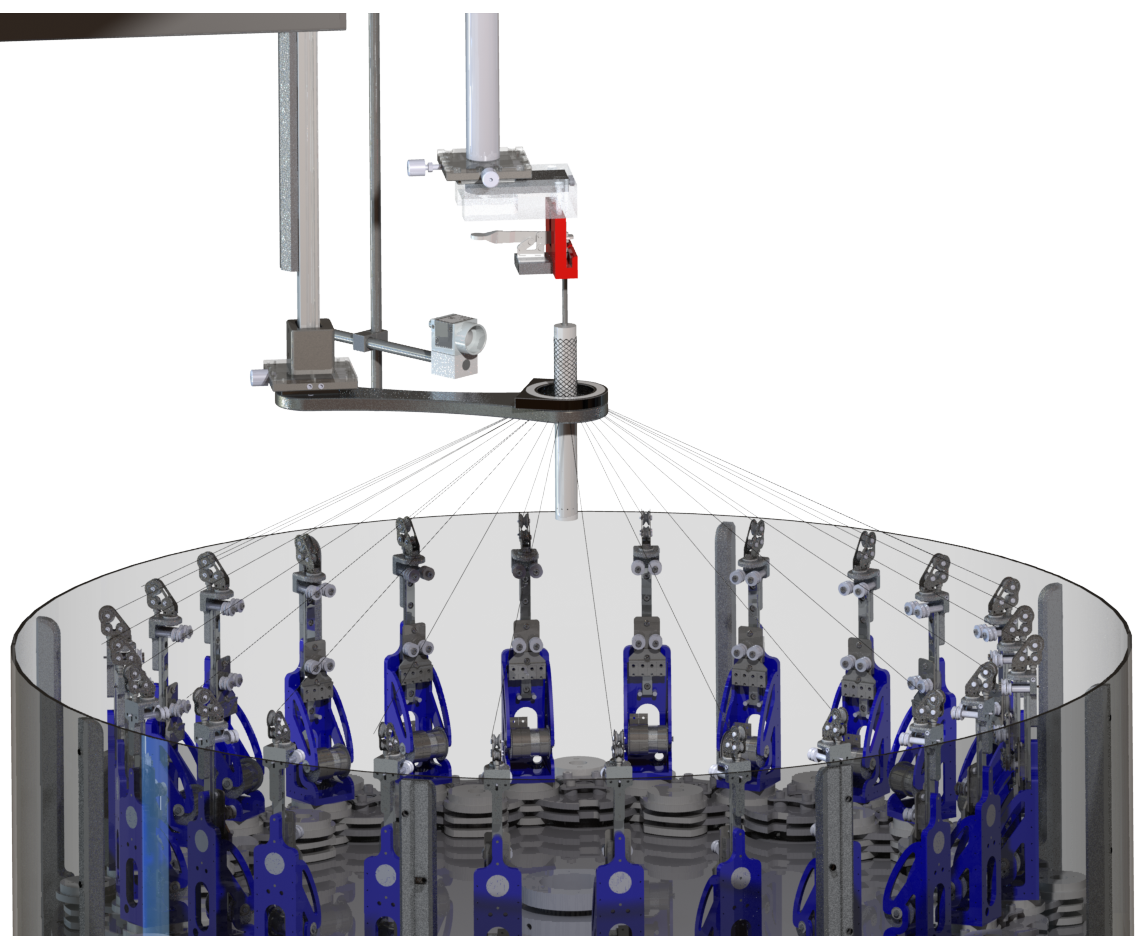
\includegraphics[width=7cm]{98_images/Flechtmaschine.png}
\caption{Aufbau einer Flechtmaschine, entnommen aus  \cite{flechtmaschine}}
\label{fig:aufbau_flechten}
\end{figure}


% Picklänge
\subsection{Picklänge}

Ein Stent kann als Gitter bestehend aus Rautenstrukturen aufgefasst werden. Eine solche Struktur, welche aus den Überkreuzungspunkten des Drahtes gebildet wird, wird als Pick bezeichnet. Die Picklänge entspricht in diesem Fall dem Abstand zwischen der oberen und unteren Ecke eines Picks. Diese Länge ist in Abbildung \ref{fig:picklaenge} dargestellt.

\begin{figure}[h!]
\centering
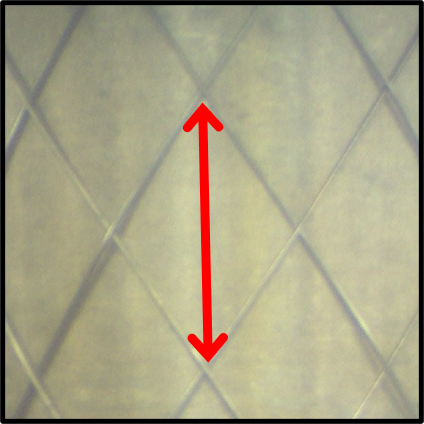
\includegraphics[width=5cm]{98_images/mittlerer_pick.png}
\caption{Veranschaulichung eines einzelnen Picks. Picklänge in rot visualisiert. Entnommen aus  \cite{flechtmaschine}.}
\label{fig:picklaenge}
\end{figure}


%
% 2.2 Histogrammausgleich
%
\section{Histogrammausgleich}\label{sec:histogramm-sec}
Der Histogrammausgleich ist ein Verfahren der Bildverarbeitung zur Kontrastverbesserung. Ziel ist es, ein Bild zu erhalten, bei dem die Bildwerte gleich verteilt sind \cite{automatische-sichtpruefung}. Ein Beispiel hierfür ist in Abbildung \ref{fig:ahe} dargestellt.

\begin{figure}[h!]
\centering
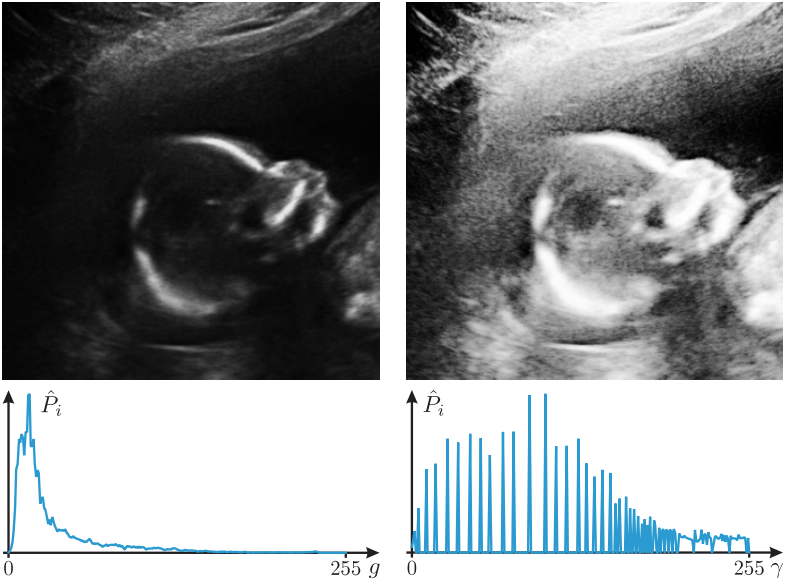
\includegraphics[width=11cm]{98_images/ahe.png}
\caption{Beispiel eines Histogrammausgleichs: links, ursprüngliches Bild; rechts, Ergebnis des Histogrammausgleichs. Darunter sind die zugehörigen Histogramme dargestellt. Entnommen aus \cite{automatische-sichtpruefung}.}
\label{fig:ahe}
\end{figure}


% AHE
\subsection{Adaptiver Histogrammausgleich}
Beim adaptiven Histogrammausgleich (engl. Adaptive Histogram Equalization) oder AHE wird diese Methode verbessert, sodass auch bei Bildern mit deutlich helleren oder dunkleren Regionen gute Ergebnisse erzielt werden können. Es werden mehrere Histogramme berechnet, um die Beleuchtungswerte im Bild neu zu verteilen. Jedes Pixel ändert sich basierend auf dem Histogramm der Region, von der es umgeben wird. Für die Anwendung an der am Rand liegenden Pixel wird ein sogenanntes Padding angewendet. In diesem Fall wird das Bild um die am Rand gespiegelten Werte erweitert. \cite{adaptive-hist-eq-and-its-variations}


% CLAHE
\subsection{Kontrastbegrenzter adaptiver Histogrammausgleich}\label{sec:clahe-sec}
Der kontrastbegrenzte adaptive Histogrammausgleich (engl. Contrast-Limited Adaptive Histogram Equalization (CLAHE)) ist eine Modifikation vom AHE. Abbildung \ref{fig:clahe} zeigt ein Beispiel für diese Methode. Hierbei wird die Kontrastverstärkung als die Ableitung der Transformationsfunktion, die Ein- und Ausgangsintensität verbindet, definiert. Der Ableitungswert eins entspricht keiner Verstärkung und höhere Werte führen zu höheren Verstärkungen. Um die Verstärkung zu begrenzen, wird das Histogramm an einer vordefinierten Höhe beschnitten. Somit wird die Steigung der Transformationsfunktion limitiert. Der Punkt, ab dem das Histogramm beschnitten wird, wird durch den Grenzwert der Steigung für die Funktion bestimmt. \cite{adaptive-hist-eq-and-its-variations}

\begin{figure}[h!]
\centering
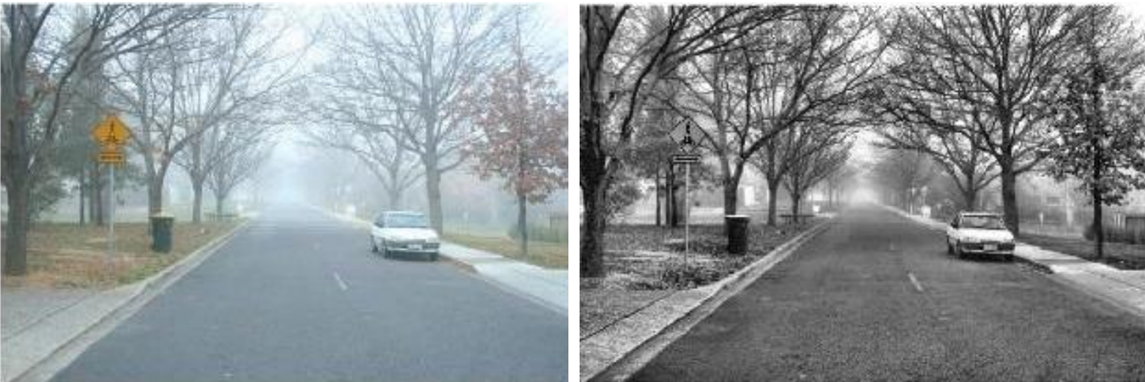
\includegraphics[width=10cm]{98_images/clahe.png}
\caption{Beispiel für die Anwendung von CLAHE: links, Originalbild mit Nebel; rechts, Bild nach der Anwendung von CLAHE. Entnommen aus \cite{clahe-based-enhancement-for-video}.}
\label{fig:clahe}
\end{figure} 


%
% 2.3 Deep Learninng
%
\section{Deep Learning}\label{sec:?}
Laut dem Wörterbuch der University of Cambridge ist Deep Learning eine Art künstlicher Intelligenz, die Algorithmen verwendet, welche auf der Funktionsweise des menschlichen Gehirns basieren \cite{cambridge_dl}. Diese neuronale Perspektive wird durch zwei Hauptideen vorangetrieben. Eine davon ist das Konzept der Nachkonstruktion der rechnerischen Prinzipien hinter dem Gehirn und die Duplizierung der Funktionalität dessen, um Intelligenz zu erschaffen. Zum anderen sollen Modelle des Deep Learnings nicht nur technischen Anwendungen dienen, sondern auch zu einem besseren Verstand über das Zerebrum und den Prinzipien, die der menschlichen Intelligenz zugrunde liegen, beitragen. \cite{Goodfellow-et-al-2016}

\begin{figure}[h!]
\centering
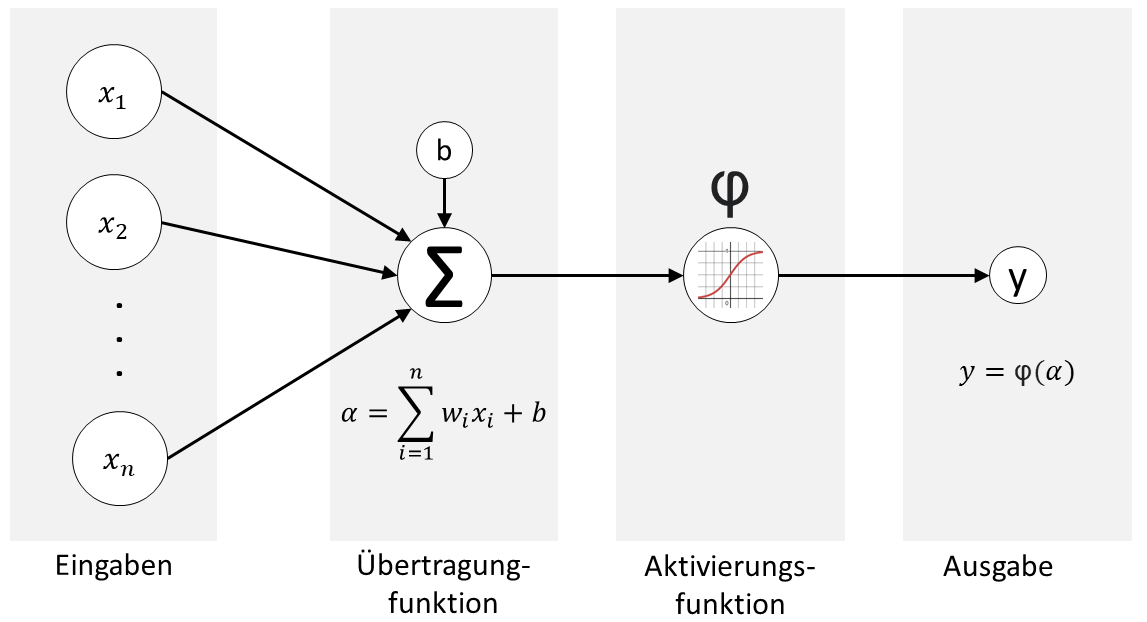
\includegraphics[width=12cm]{98_images/perceptron.png}
\caption{Schematischer Aufbau eines künstlichen neuronalen Netzes, das als einschichtiges Perzeptron-Netz modelliert wird. In Anlehnung an  \cite{Deep-Learning-mit-tf-keras-und-tfjs}.}
\label{fig:perceptron}
\end{figure}

\mypar Diese Modelle werden mithilfe künstlicher Neuronen gebildet, die auf mehreren Ebenen miteinander verbunden sind. Hierbei wird jede Nervenzelle als sogenanntes Perzeptron (siehe Abbildung \ref{fig:perceptron}) modelliert, bei dem die Dendriten des biologischen Neurons durch eine Schicht mit Eingaben gestaltet werden. Das Perikaryon wird durch die Übertragungsfunktion, das Axon durch die Ausgabe und die inhibitorischen bzw. exzitatorischen Eigenschaften der Synapse werden durch die Gewichte repräsentiert. Zur erwähnten Eingabe gehört auch ein Bias, welches zur Summe aller Eingaben addiert wird, bevor die Gleichung \ref{eq:uebertragungsfunktion_perzeptron} in die Aktivierungsfunktion eingegeben wird. Diese bestimmt den Schwellenwert, bei dem die Nervenzelle aktiviert wird \cite{Deep-Learning-mit-tf-keras-und-tfjs}. Somit war das von Frank Rosenblatt entworfene Perzeptron das erste Modell, welches in der Lage war, anhand von Beispielen die Gewichte der einzelnen Kategorien zu definieren \cite{The-Perceptron}.

\begin{equation}\label{eq:uebertragungsfunktion_perzeptron}
\alpha=\sum_{i=1}^{n}w_i x_i + b
\end{equation}

Mithilfe solcher künstlichen Neuronen kann ein neuronales Netz wie in Abbildung \ref{fig:mlp-fig} aufgebaut werden. Das abgebildete Netzwerk besteht aus drei Schichten: die Eingabeschicht, eine Zwischenschicht und eine Ausgabeschicht. Eine Eingabe wird in das Netz über die zwei Neuronen der ersten Schicht eingespeist und an die Zwischenschicht weitergeleitet. Von dort wird sie an die Ausgabeschicht geleitet, an der die Ausgabe des Netzwerks dargestellt wird.

\begin{figure}[h!]
\centering
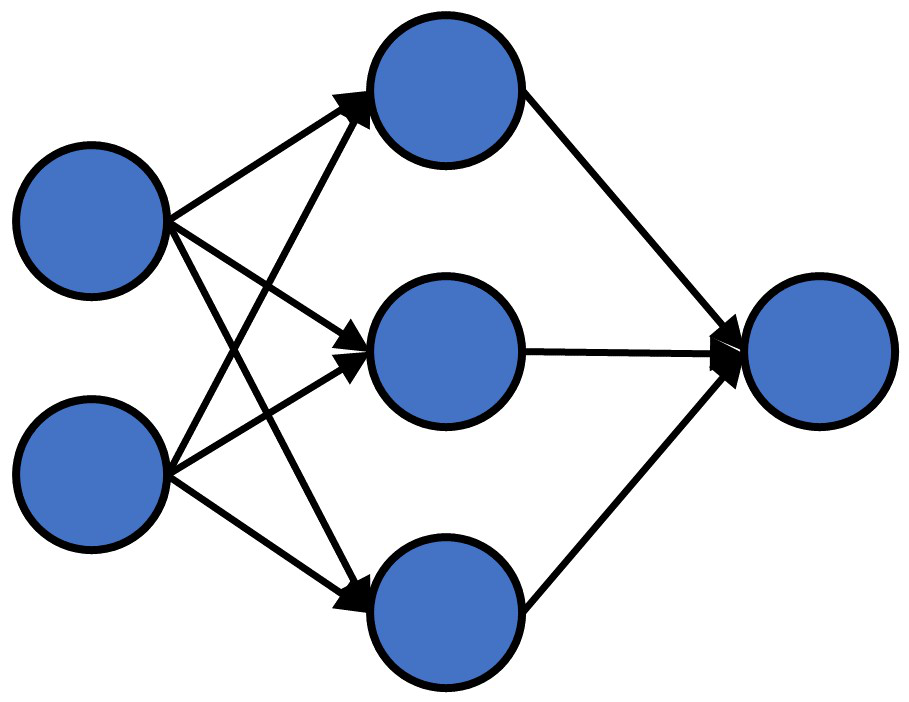
\includegraphics[width=6cm]{98_images/mlp.png}
\caption{Aufbau eines neuronalen Netzes mit zwei Neuronen für die Eingabe und einem für die Ausgabe}
\label{fig:mlp-fig}
\end{figure}


%
% Training eines Neuronalen Netzes
%
\subsection{Training eines neuronalen Netzes}
Das Training eines neuronalen Netzes ist der Prozess, bei dem die Parameter so gesetzt werden, dass die Differenz zwischen den Ist- und den Soll-Werten möglichst minimiert wird. Die Ausgabe des Netzes, also der Ist-Wert, wird mit der gewünschten Ausgabe (Soll-Wert), welche als Label bezeichnet wird, verglichen. \cite{cnns-an-overview-and-application-in-radiology}

\mypar Zu Beginn des Trainings wird ein Stapel (engl. batch) von Bildern wird vom Eingang zum Ausgang des Netzes vorwärts propagiert. Darauffolgend wird die Leistung des Modells mithilfe einer Fehlerfunktion berechnet. Diese misst die Differenz zwischen den Netzausgaben und den Labels. Im Anschluss werden die erlernbaren Parameter des Netzwerks anhand des Backpropagation-Algorithmus \cite{rumelhart1985learning} und dem Gradientenverfahren (siehe Abschnitt \ref{sec:gradient-descent-sec}) für Optimierungsprobleme angepasst. \cite{cnns-an-overview-and-application-in-radiology}

\mypar Der Ablauf des Trainings eines neuronalen Netzes wird in drei Phasen aufgeteilt, wodurch es drei unterschiedliche Datensätze benötigt: einen Test-, einen Validierungs- und einen Testdatensatz. Die Trainingsdaten werden verwendet, um das Modell zu trainieren. In der Validierungsphase wird bestimmt, wie gut das neuronale Netz trainiert wurde. Zuletzt wird der Testdatensatz für die Bewertung des Generalisierungsfehlers des Modells verwendet. \cite{hastie2009elements}


% MAE
\subsubsection{Mittlerer absoluter Fehler}\label{mae-section}
Der mittlere absolute Fehler (engl. Mean Absolute Error, kurz MAE) gibt den Durchschnitt aller Absolutbeträge der einzelnen Abweichungen zwischen der Netzausgabe und dem Label an. Für $n$ Testinstanzen wird dieser wie folgt berechnet:

\begin{equation}\label{eq:mae}
\text{MAE}=\frac{1}{n} \sum_{i=1}^{n} |(y_i - \lambda(x_i)|,
\end{equation}

\mypar wobei $y_i$ und $\lambda(x_i)$ den Soll- und Ist-Wert für $x_i$ darstellen. \cite{sammut2011encyclopedia}


% MSE
\subsubsection{Mittlerer quadratischer Fehler}
Beim mittleren quadratischen Fehler (engl. Mean Squared Error, kurz MSE) wird die quadratische Abweichung der Netzausgaben zum Soll-Wert über $n$ Testinstanzen wie folgt bestimmt: 

\begin{equation}\label{eq:mse}
\text{MSE}=\frac{1}{n} \sum_{i=1}^{n}(y_i-\lambda(x_i))^2.
\end{equation}

Die Bedeutungen für $y_i$, $\lambda(x_i)$ und $x_i$ sind analog zu \ref{mae-section}. \cite{sammut2011encyclopedia}

\mypar Der Unterschied zwischen den zwei vorgestellten Verlustfunktionen wird in Abbildung \ref{fig:mae-mse} anhand zwei beispielhafter Verläufe aufgezeigt. Der mittlere absolute Fehler steigt linear mit einem zunehmenden Fehler an. Im Gegensatz dazu steigt die Funktion beim MSE exponentiell mit einer Zunahme des Fehlers. Dadurch bestraft der mittlere quadratische Fehler große Abweichungen mehr als kleine.

\begin{figure}[h!]
\centering
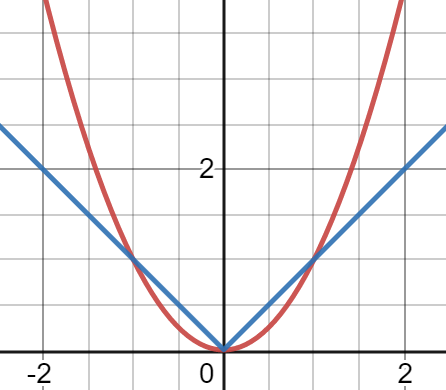
\includegraphics[width=5cm]{98_images/mae_mse.png}
\caption{Beispielhafter Verlauf für den mittleren absoluten Fehler (blau) und den mittleren quadratischen Fehler (rot).}
\label{fig:mae-mse}
\end{figure}


% Gradient Descent
\subsubsection{Gradientenverfahren}\label{sec:gradient-descent-sec}
Das Gradientenverfahren (engl. gradient descent) ist ein Optimierungsalgorithmus für das iterative Anpassen der erlernbaren Parameter eines neuronalen Netzes, um den Verlust des Netzwerks möglichst zu minimieren. Der Gradient der Verlustfunktion gibt die Richtung an, in der die negative Steigung der Funktion am größten ist. So werden die Filterkerne und Gewichte in diese Richtung des Gradienten angepasst. Die Schrittgröße wird anhand der Lernrate, ein positiver Skalar, bestimmt. Eine Darstellung dieses Verfahrens wird in Abbildung \ref{fig:grad-descent} dargestellt. Bei einer zu großen Lernrate kann die Verlustfunktion steigen anstatt zu sinken. Andernfalls wird das Training eines Netzes bei einer zu kleinen Lernrate langsamer und es besteht die Gefahr, bei einem hohen Fehler dauerhaft stecken zu bleiben \cite{Goodfellow-et-al-2016}. \cite{cnns-an-overview-and-application-in-radiology}

\begin{figure}[h!]
\centering
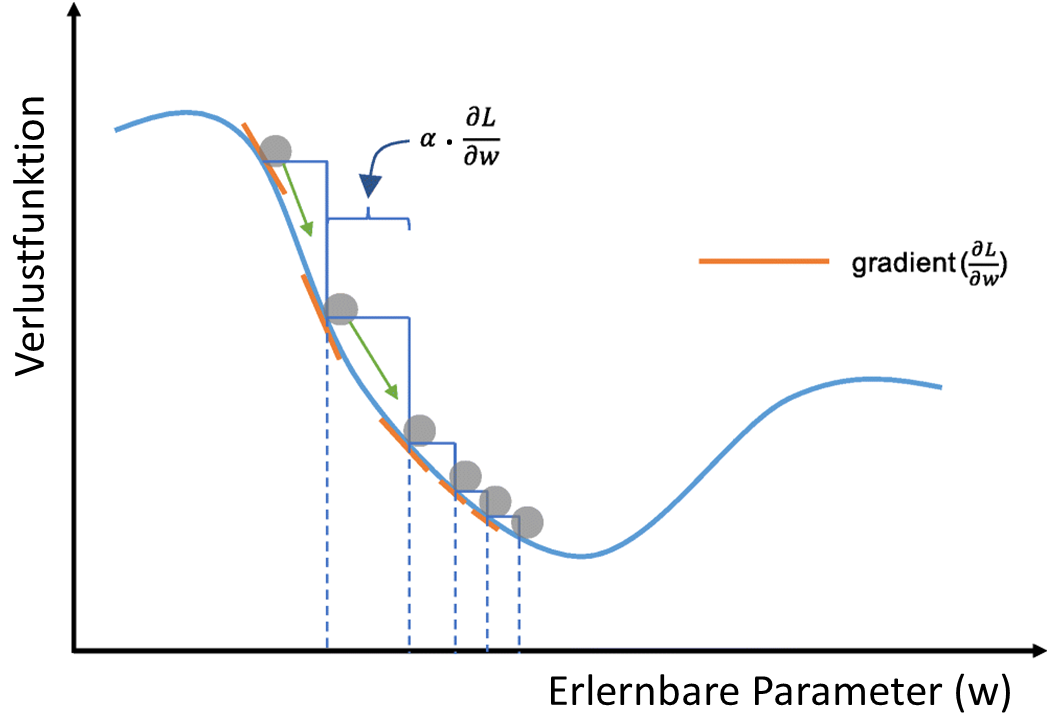
\includegraphics[width=10cm]{98_images/gradientenverfahren.png}
\caption{Verlauf des Gradientenverfahrens mit einer Lernrate $\alpha$, einer Verlustfunktion L und den Parametern w. Ursprüngliches Bild aus \cite{cnns-an-overview-and-application-in-radiology}.}
\label{fig:grad-descent}
\end{figure}

\mypar Eine solche Aktualisierung der Parameter wird in Gleichung \ref{eq:gradient-descent} formuliert. In diesem Fall steht $w$ für einen einzelnen Parameter, $\alpha$ für die Lernrate und $L$ für die Verlustfunktion.

\begin{equation}\label{eq:gradient-descent}
w:=w-\alpha \cdot \frac{\partial L}{\partial w}. 
\end{equation}


% Adam
\subsubsection{Adam}
Der Optimierungsalgorithmus Adam ist eine Weiterentwicklung des Gradientenverfahrens. Dieses Verfahren berechnet einzelne anpassungsfähige Lernraten für unterschiedliche Parameter und basiert auf zwei anderen Algorithmen und entnimmt deren Vorteile; AdaGrad und RMSProp. Adaptive Gradient (AdaGrad) stellt eine feste Lernrate pro Parameter fest und verbessert die Leistung bei sogenannten ''sparse''-Gradienten \cite{adagrad}. Laut Elibol et al. \cite{variance-red-w-sparse-grads} sind damit Gradienten gemeint, die eine geringe Anzahl an großen Koordinaten besitzen. Root Mean Square Propagation (RMSProp) verwendet den Durchschnitt des quadratischen Gradienten, um die Parameter anzupassen \cite{rmsprop}. Adam ist rechnerisch effizient, benötigt wenig Speicher und ist gut für Anwendungen mit vielen Daten und Parametern geeignet. \cite{adam-paper}

\mypar Die Parameteranpassungen werden wie folgt durchgeführt:

\begin{equation}\label{eq:adam1}
\theta_t = \theta_{t-1}-\alpha \frac{\hat{m}_t}{\sqrt{\hat{v}_t}+\epsilon}
\end{equation}

\mypar mit

\begin{equation}\label{eq:adam2}
\begin{aligned}
g_t = \nabla_{\theta} f_t(\theta_{t-1}) \\
m_t = \beta_1 m_{t-1} + (1-\beta_1)g_t \\
v_t = \beta_2 v_{t-1} + (1-\beta_2)g^2_t \\
\hat{m}_t = \frac{m_t}{1-\beta^t_1} \\
\hat{v}_t = \frac{v_t}{1-\beta^t_2}
\end{aligned}
\end{equation}

\mypar $\alpha$ steht für die Lernrate mit einem Wert von 1e-3 in der Veröffentlichung. $\epsilon$ ist eine sehr kleine Zahl, üblicherweise 1e-8 or 1e-10, um eine Nulldivision zu vermeiden. $\beta_1$ und $\beta_2$ sind die exponentiellen Abnahmeraten für die Momentenschätzwerte erster und zweiter Ordnung und betragen üblicherweise 0,9 bzw. 0,999. Nach der Berechnung des Gradienten $g_t$ zum Zeitpunkt $t$ werden die verzerrten Schätzwerte für das statische Moment $m_t$ und für das Trägheitsmoment $v_t$ aktualisiert. Darauffolgend wird die Verzerrung dieser Werte korrigiert und es ergeben sich $\hat{m}_t$ und $\hat{v}_t$. Aus diesen Anteilen kann der angepasste Parameter mit Gleichung \ref{eq:adam1} bestimmt werden. \cite{Goodfellow-et-al-2016}


% Regularisierung
\subsubsection{Regularisierung}\label{sec:regularisierung-sec}
Neuronale Netze werden nach dem Training auf Bilder oder Daten, die in dem Modell noch nie zuvor eingegeben wurden, getestet. Somit kann untersucht werden, wie gut ein Modell Informationen generalisieren kann. Ein Netzwerk mit einer guten Generalisierungsfähigkeit kann gute Ergebnisse auf diesen Testdaten erzielen. Das sogenannte Overfitting tritt auf, wenn ein Modell die Trainingsdaten zwar gut verarbeiten kann, aber nicht die Testdaten. In diesem Fall hat sich das neuronale Netz viel zu gut an die Trainingsdaten angepasst und kann noch nie gesehene Muster deshalb schlecht verarbeiten. Abbildung \ref{fig:alexnet-log-scale} zeigt den Verlauf eines solchen Trainings. Im Gegensatz dazu wird bei einer schlechten Leistung sowohl im Trainings-, als auch im Testdatensatz von Underfitting gesprochen. Um dieses fundamentale Problem des Deep Learnings zu bekämpfen, gibt es mehrere Methoden die angewendet werden können, wie Daten-Augmentation, Verwendung von mehr Trainingsdaten, Regularisierung, Batch Normalization (siehe \ref{batch-normalization-sec}) oder Reduzieren der Modellkomplexität \cite{overfitting-mechanism-and-avoidance-in-dnl}. Im Folgenden wird auf einige Techniken der Regularisierung tiefer eingegangen. \cite{cnns-an-overview-and-application-in-radiology}

\begin{figure}[h!]
\centering
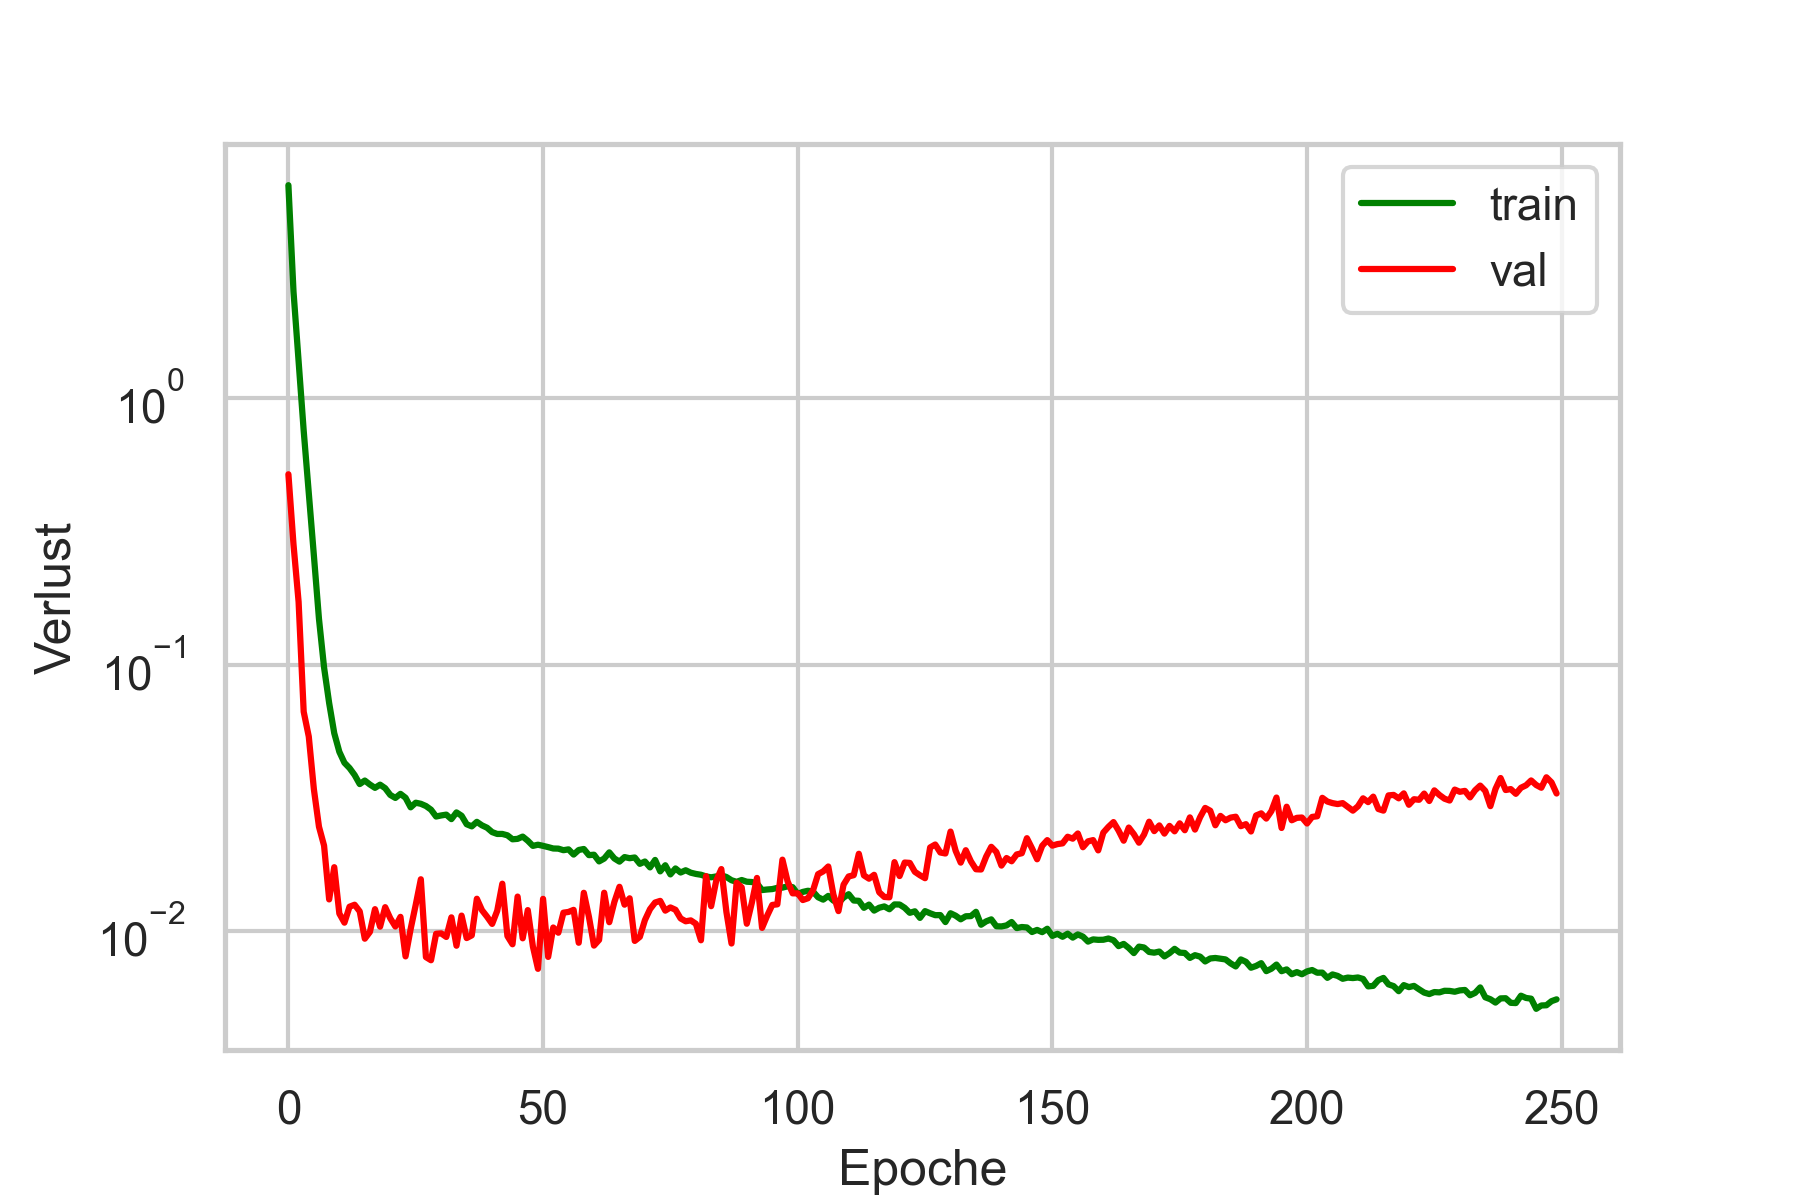
\includegraphics[width=12cm]{98_images/AlexNet_log_scale.png}
\caption{Beispielhafter Verlauf eines Trainings mit Overfitting. Der Trainingsloss sinkt über den gesamten Vorgang, demgegenüber fängt der Validierungsloss ab etwa der 50. Epoche an zu steigen.}
\label{fig:alexnet-log-scale}
\end{figure}

\mypar Eine verbreitete Methode ist das Early Stopping, welches für ein vorzeitiges Abbrechen des Trainingvorgangs, um Overfitting zu vermeiden, sorgt. Jedes Mal, wenn der Fehler auf dem Validierungssatz verringert wird, wird eine Kopie der Parameter gespeichert. Dieser Algorithmus beendet das Training, sobald das Modell nach einer vorgegebenen Anzahl an Iterationen keine besseren Ergebnisse auf die Validierungsdaten erzielt. Das Modell mit den besten Parametern wird zurückgegeben. \cite{Goodfellow-et-al-2016}

\mypar Das Dropout ist ein weiteres Instrument der Regularisierung. Beim Dropout wird während des Trainings ein Neuron und dessen Verbindungen mit einer vorgegebenen Ausfallwahrscheinlichkeit $p$ deaktiviert, wodurch das Neuron von der Modellarchitektur temporär ausgeschlossen wird. Während der Testphase sind alle Neuronen und Verbindungen aktiv, doch die Gewichte werden mit $p$ skaliert. Hiermit wird eine übermäße Abhängigkeit des Netzes von bestimmten Verbindungen vermieden. Dadurch wird anhand dieser Methode ein Ensemble trainiert, welches aus mehreren Teilnetzen besteht. Das Ensemble enthält alle möglichen Netzwerke, die durch Entfernen von Einheiten mit der Ausfallwahrscheinlichkeit gefertigt werden können. \cite{dropout}

\mypar Darüber hinaus sind die L1- und L2-Regularisierungen ein weiteres Mittel, um Overfitting zu vermeiden. Bei den Dabei handelt es sich um Funktionen, die zur Verlustfunktion hinzugefügt werden. Die L1-Regularisierung entspricht der Summe der Beträge, also die L1-Normen, der Parameter. Dies führt zu einer Lösung, bei der einige Parameter einen optimalen Wert von Null haben. Die Lösung ist also dünnbesetzter, wodurch sich das Netzwerk auf die Erkennung bedeutsamer Merkmale begrenzt. Bei der L2-Regularisierungsfunktion wird die L2-Norm der Parameter betrachtet. Dies verhindert das Entstehen von Gewichten mit zu hohen Werten. Formal sind die Bestrafungen der L1- und L2-Regularisierungen für eine Gewichtung $w_k$ in Gleichung \ref{eq:regularisierung-1} und Gleichung \ref{eq:regularisierung-2} definiert. \cite{deep-neural-network-regularization}

\begin{equation}\label{eq:regularisierung-1}
\Omega (W^{(p)})_{l1} = \vert w \vert  = \sum_{k=1}^{m} \vert w_k \vert
\end{equation}

\begin{equation}\label{eq:regularisierung-2}
\Omega(W^{(p)})_{l2} \equiv \Vert W \Vert^2_2
\end{equation}


% CNNs
\subsection{Faltende neuronale Netze}
Faltende neuronale Netze (kurz CNN) sind vorwärtsgekoppelte Netzwerkarchitekturen, weil sie durch unidirektionale Verbindungen zwischen den Neuronen ausgezeichnet werden. Dementsprechend führt kein Pfad aus dem Ausgang eines Neurons zum Eingang dessen oder zu einer vorherigen Schicht des Netzes; der Aufbau stellt einen azyklischen Graphen dar. Da sie von der von Hubel und Wiesel 1959 \cite{hubel-wiesel} erforschten Funktionsweise der Informationsverarbeitung im visuellen Kortex inspiriert sind, eignen sie sich besonders für Bilder. In dieser Region des Gehirns werden globale Probleme in mehrere kleinere und daher leichter zu lösende Schritte verwandelt. \cite{Deep-Learning-mit-tf-keras-und-tfjs}

\mypar Eine der ersten Implementierungen eines CNN ist das 1989 von LeCun et al. \cite{lenet-1} publizierte und neun Jahre später in \cite{lenet-2} verbesserte LeNet-5 Modell. Seitdem sind mehrere Architekturen und somit auch Schichten entworfen worden, mit dem Ziel, Schwierigkeiten beim Trainieren der Netze zu beseitigen und deren Effektivität zu steigern. \cite{recent-advances-in-cnns}


% Convolutional Layer
\subsubsection{Convolutional Layer}
Das Convolutional Layer (engl. Convolutional Neural Network, kurz Conv) ist ein grundlagender Bestandteil aller CNN-Architekturen, weil es für das Extrahieren von Eigenschaften sorgt. Dies basiert auf der mathematischen Operation der Faltung \cite{cnns-an-overview-and-application-in-radiology}. Die Faltung innerhalb der Schicht wird typischerweise wie in Gleichung \ref{eq:faltung} notiert.

\begin{equation}\label{eq:faltung}
S(i,j)=(I*K)(i,j)=\sum_{m}\sum_{n}I(m,n)K(i-m,j-n)
\end{equation}

\mypar Hierbei wird ein zweidimensionales Bild $I$ mit einem ebenfalls zweidimensionalen Filterkern gefalten und ergibt somit eine sogenannte Feature Map (siehe Abbildung \ref{fig:convolution}) \cite{Goodfellow-et-al-2016}. Der Filter wird auf die gesamte Eingabe angewendet. Durch die Wiederholung des Vorgangs mit unterschiedlichen Kernen kann eine willkürliche Anzahl an Feature Maps erzeugt werden, welche unterschiedliche Eigenschaften der Eingabe darstellen. So können unterschiedliche Feature Maps beispielsweise Augen, Mund und Nase auf Bildern von Gesichten hervorheben. Üblicherweise werden Filter der Größe $3 \times 3$ verwendet, doch diese lässt sich modifizieren. Der Abstand zwischen zwei Positionen an denen der Filterkern angewendet wird, wird durch dem Stride festgelegt. \cite{cnns-an-overview-and-application-in-radiology}

\begin{figure}[h!]
\centering
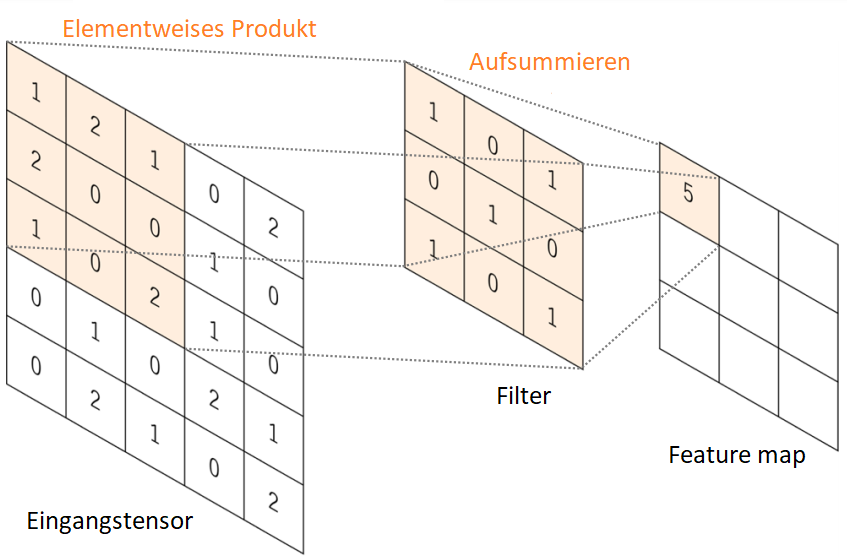
\includegraphics[width=11cm]{98_images/convolution.png}
\caption{Beispiel einer Faltungsoperation mit einen $3 \times 3$ Filter. Entnommen und neu beschriftet aus  \cite{cnns-an-overview-and-application-in-radiology}.}
\label{fig:convolution}
\end{figure}

\mypar Da die durch die Anwendung des Filters enstandene Feature Map eine reduzierte Höhe und Breite gegenüber dem ursprünglichem Bild aufweist, kann beispielsweise zero-Padding benutzt werden. An den Rändern der Eingabe werden Reihen und Spalten mit Nullen hinzugefügt, sodass die Dimension des Tensors, welches eine bestimmte Anzahl von Vektoren auf einen Vektor abbildet, beibehalten wird. \cite{an-introduction-to-cnns}


% Aktivierungsfunktionen
\subsubsection{Aktivierungsfunktionen}
Ausgaben einer linearen Operation wie die Faltung werden darauffolgend in eine nichtlineare Aktivierungsfunktion eingesetzt. Die Auswahl der Funktion hat einen signifikanten Einfluss auf das Training und die Leistung des Modells \cite{searching-for-act-functions}. Im Rahmen dieser Arbeit sind folgende drei Funktionen relevant. 

\mypar Die Sigmoid-Aktivierungsfunktion aus Gleichung \ref{eq:sigmoid} wird oftmals auch als logistische Funktion bezeichnet. Es handelt sich um eine begrenzt differenzierbare reelle Funktion, welche für reelle Eingabewerte definiert ist und Werte zwischen null und eins ausgibt. \cite{activation-functions}

\begin{equation}\label{eq:sigmoid}
f(x)=\frac{1}{1+e^{-x}}
\end{equation}

 Eine der bekanntesten Aktivierungsfunktionen ist die in Gleichung \ref{eq:relu} aufgezeigte Rectified Linear Unit (ReLU) \cite{imagenet-class-w-deep-cnns}. Künstliche neuronale Netze mit ReLU sind einfacher zu optimieren, als Netze, welche zuvor veröffentlichten Funktionen verwenden, weil die mathematischen Operationen der Funktion simpler sind \cite{searching-for-act-functions}.

\begin{equation}\label{eq:relu}
f(x)=\text{max}(0,x)
\end{equation}

\mypar Das Exponential Linear Unit (ELU) wurde 2015 eingeführt (siehe Gleichug \ref{eq:elu}) und erlaubt ein schnelleres und präziseres Lernen in Netzen. Im Vergleich zur ReLU-Funktion können ELUs auch negative Werte aufzeigen, beschleunigen das Training und verbessern die Generalisierung der Netze. \cite{elus}

\begin{equation}\label{eq:elu}
f(x)=
\begin{cases}
x & \text{, x} > \text{0} \\
\alpha(\text{exp}(x)-1) & \text{, x} \leqslant \text{0}
\end{cases}
\text{	für } \alpha > \text{0}
\end{equation}


% Pooling Layer
\subsubsection{Pooling Layer}
Ziel des Pooling Layers ist, die Dimensionalität der Eingabe zu reduzieren und gleichzeitig möglichst keinen Informationsverlust zu erleiden \cite{understanding-of-a-cnn}. Eine Invarianz gegen kleine Verschiebungen und Verzerrungen wird eingeführt und die Anzahl der erlernbaren Parameter sinkt. Ähnlich zur Faltung, sind Stride, Padding und die Größe des Filters Hyperparameter beim Pooling. Damit ist ein Parameter gemeint, dessen Wert zur Steuerung des Trainings verwendet wird. Eine der meist verbreiteten Formen ist das Max Pooling, welche in Abbildung \ref{fig:pooling-layer} angewendet wird, bei dem der höchste Wert innerhalb des Bereiches übergeben wird. Eine weitere Variante ist das Average Pooling, bei dem der durchschnittliche Wert aller Werte im Bereich übernommen wird. \cite {cnns-an-overview-and-application-in-radiology}

\begin{figure}[h!]
\centering
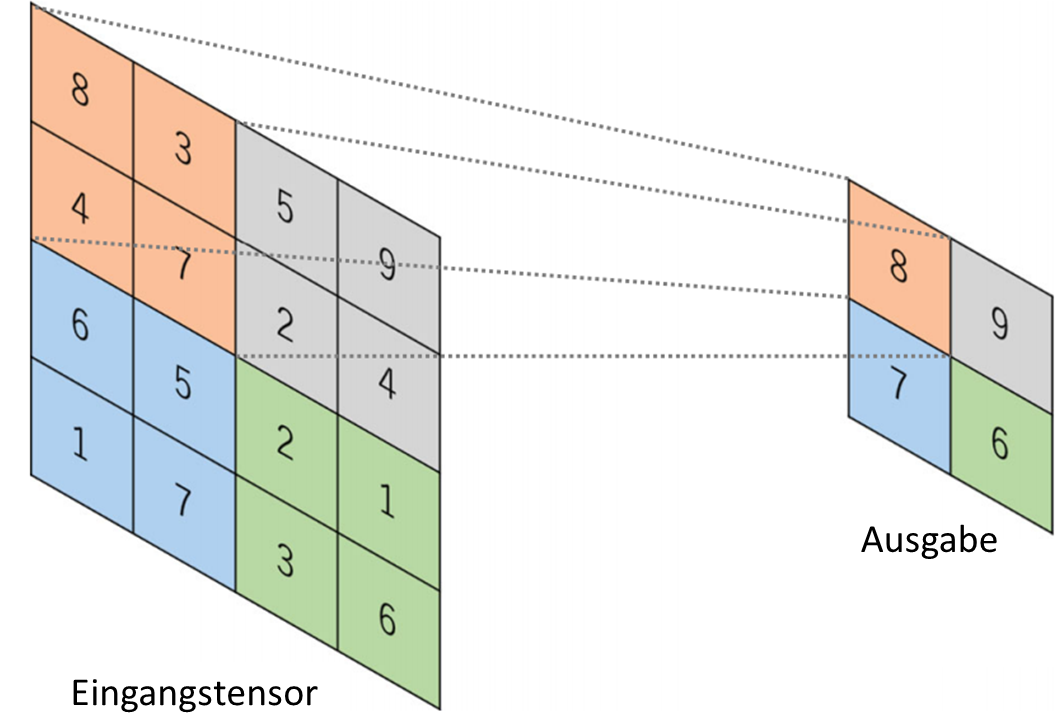
\includegraphics[width=10cm]{98_images/pooling_layer.png}
\caption{Beispiel zur Anwendung von Max Pooling. Ursprüngliches Bild aus \cite{cnns-an-overview-and-application-in-radiology}.}
\label{fig:pooling-layer}
\end{figure}


% Fully Connected Layer
\subsubsection{Fully Connected Layer}
Beim Fully Connected Layer (auch Dense Layer genannt) sind alle Neuronen direkt mit allen Neuronen der zwei benachbarten Schichten verbunden. Ein solcher Aufbau wird in Abbildung \ref{fig:fc-layer} aufgezeigt. Dies ist ähnlich zur Form in der die Nervenzellen beim einem traditionellen neuronalen Netz angeordnet sind. Da dieser Aufbau viele Paramter einbezieht, können sie eine lange Zeit beim Trainieren beanspruchen. \cite{understanding-of-a-cnn}

\begin{figure}[h!]
\centering
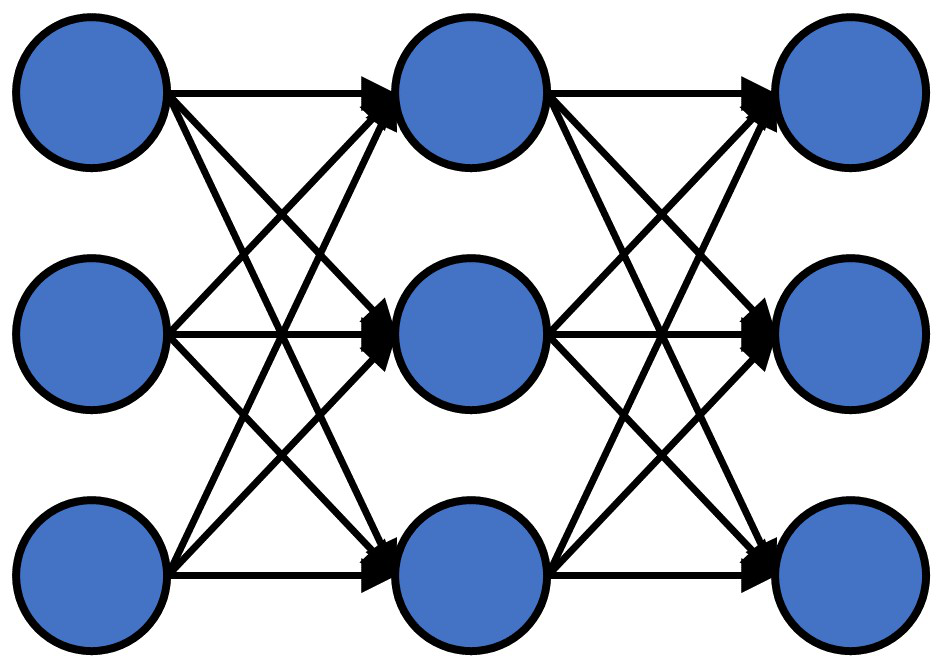
\includegraphics[width=5cm]{98_images/fc_layer.png}
\caption{Aufbau eines Fully Connected Layers.}
\label{fig:fc-layer}
\end{figure}


% Batch Normalization Layer
\subsubsection{Batch Normalization Layer}\label{batch-normalization-sec}
Das von Ioffe et al. \cite{pmlr-v37-ioffe15} entworfene Batch Normalisation Layer (kurz BN) hat die Aufgabe die Eingänge in das Layer zu normalisieren. Darunter wird eine Transformation der Werte in einen bestimmten Bereich mit Erwartungswert null und Varianz eins verstanden. Dies wird durch die Anwendung von Gleichungen \ref{eq:ioffe1}, \ref{eq:ioffe2}, \ref{eq:ioffe3} und \ref{eq:ioffe4} auf eine Datenmenge $\mathcal{B} = \{x_1, ..., x_m \}$ erzielt. \cite{pmlr-v37-ioffe15}

\begin{equation}\label{eq:ioffe1}
\mu_\mathcal{B} \gets \frac{1}{m} \sum_{i=1}^{m}x_i
\end{equation}

\begin{equation}\label{eq:ioffe2}
\sigma^2_\mathcal{B} \gets \frac{1}{m} \sum_{i=1}{m}(x_i - \mu_\mathcal{B})^2
\end{equation}

\begin{equation}\label{eq:ioffe3}
\hat{x}_i \gets \frac{x_i - \mu_\mathcal{B}}{\sqrt{\sigma^2_\mathcal{B} + \epsilon}}
\end{equation}

\begin{equation}\label{eq:ioffe4}
y_i \gets \gamma \hat{x}_i + \beta \equiv \textbf{BN}_{\gamma , \beta}(x_i)
\end{equation}

\mypar Als erstes wird $\mu_\mathcal{B}$, der Durchschnitt aller Werte berechnet und daraus wird $\sigma^2_\mathcal{B}$, die Varianz der Eingaben, bestimmt (Gleichung \ref{eq:ioffe2}). Daraufhin werden die Werte normalisiert und die transformierten Ausgaben ergeben sich in Gleichung \ref{eq:ioffe4} aus einer Skalierung und Verschiebung im Zielbereich. Hierbei sind $\gamma$ und $\beta$ erlernbare Parameter und $\epsilon$ eine Konstante mit einem sehr geringen Wert, um Division durch Null zu vermeiden und somit numerische Stabilität zu gewährleisten. \cite{pmlr-v37-ioffe15}

\mypar Batch Normalization reduziert das Risiko eines Overfittings und verbessert den Verlauf von Gradienten über das Netz. Dies erlaubt die Verwendug höherer Lernraten, wodurch die Trainingszeiten der neuronalen Netze reduziert  werden. Zudem sinken Batch Normalization Layern das Bedürfnis nach Dropout \cite{recent-advances-in-cnns}. Für eine lineare Regression wird außerdem durch dessen Verwendung eine bessere Generalisierung laut Lathuiliere et al. \cite{lathuiliere2019comprehensive} erzielt.


% Inception Layer
\subsubsection{Inception Layer}
Das in \cite{going-deeper-with-convolutions} eingeführte Inception Layer besteht aus einer parallelen Anordnung von drei Convolutional Layern und einem Pooling Layer mit den Filtergrößen $1\times1$, $3\times3$, $5\times5$ und $3\times3$. Diese Operationen werden zusammen für die gleiche Eingabe ausgeführt und die jeweiligen Ausgänge werden gemeinsam verkettet. Der entsprechende Aufbau ist in Abbildung \ref{fig:inception1} zu sehen. \cite{going-deeper-with-convolutions}

\begin{figure}[h!]
\centering
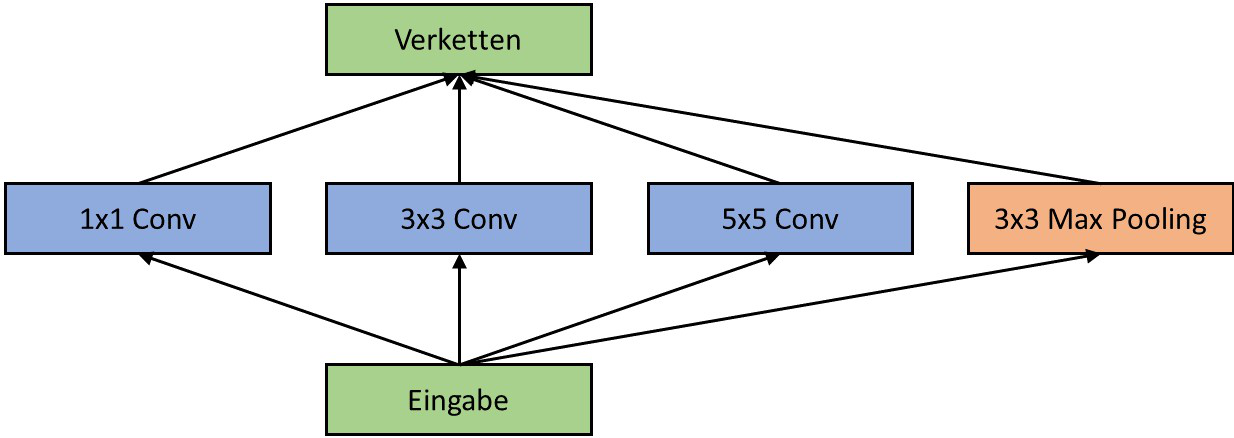
\includegraphics[width=12cm]{98_images/inception_layer1.png}
\caption{Aufbau des Inception Layer nach \cite{going-deeper-with-convolutions} ohne 1x1 Convolution.}
\label{fig:inception1}
\end{figure}

Aufgrund des Rechenaufwands von 5x5 Convolutional Layern, kann die Architektur aus Abbildung \ref{fig:inception1} mit 1x1 Convolutional Schichten zum Aufbau in Abbildung \ref{fig:inception2} erweitert werden. Somit sinkt die benötigte Rechenleistung und es wird eine kleinere Dimension der Ausgabe erzielt. \cite{going-deeper-with-convolutions}

\begin{figure}[h!]
\centering
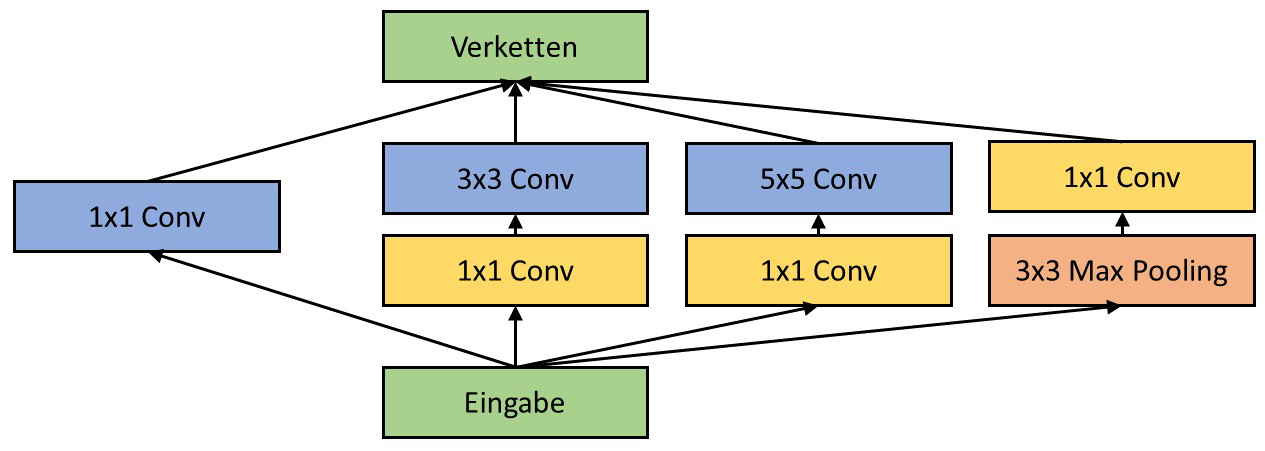
\includegraphics[width=12cm]{98_images/inception_layer2.png}
\caption{Aufbau des Inception Layer nach \cite{going-deeper-with-convolutions} mit 1x1 Convolution.}
\label{fig:inception2}
\end{figure}

\mypar Die Weiterentwicklung dieses Moduls hat zu einer Diversifikation bei den Varianten geführt. So entstanden die Inception-A, Inception-B, Inception-C, Reduction-A und Reduction-B Module. Im Vergleich zu den zwei Jahre älteren Versionen haben diese einen geringeren Trainingsaufwandaufwand. \cite{inception-inceptionresnet-and-the-impact-of-residual-connections-on-learning}


% Separable Convolution Layer
\subsubsection{Separable Convolution Layer}
Das Separable Convolution Layer ist, vom Aufbau her, ähnlich zu dem eines Inception Moduls, welches nur eine Größe von Filtern verwendet und keinen Pooling Layer besitzt. Dies kann als gesamte $1\times1$ Convolution, die von weiteren einzelnen Convolutional Layern gefolgt wird, gesehen werden. Die nachfolgenden Schichten arbeiten auf nichtüberlappenden Segmenten der Ausgabe. Beide Operationen werden von einer ReLU-Aktivierungsfunktion gefolgt. Ein Beispiel für eine solche Architektur ist in Abbildung \ref{fig:sep_conv} aufgezeigt. \cite{xception-dl-with-depthwise-sep-conv}

\begin{figure}[h!]
\centering
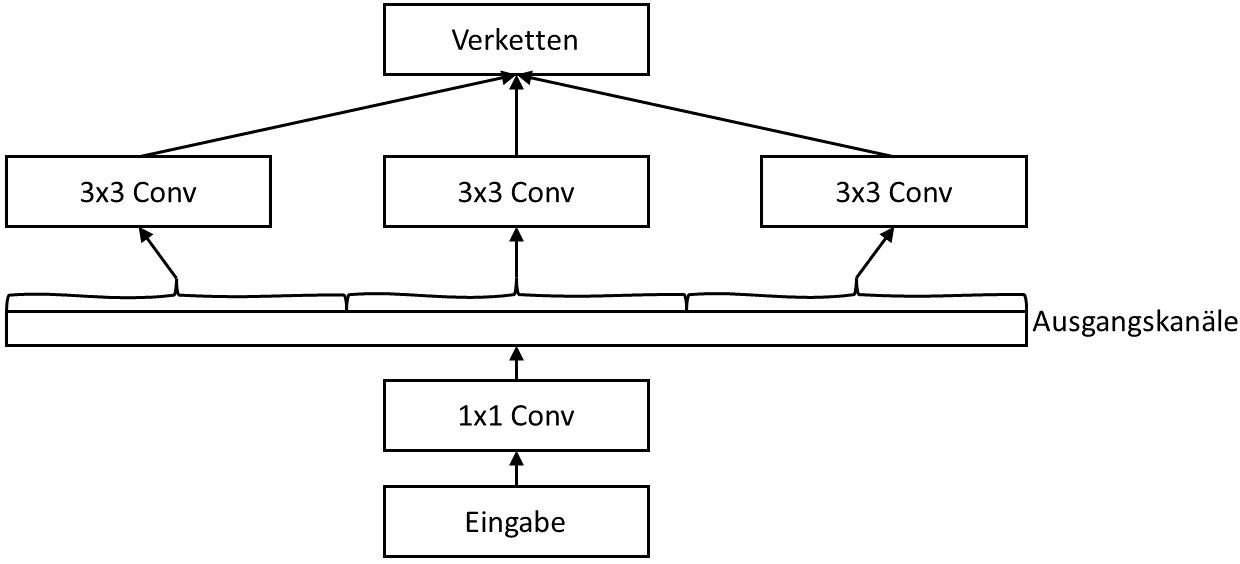
\includegraphics[width=12cm]{98_images/sep_conv.png}
\caption{Beispiel eines Separable Convolution Layer nach \cite{xception-dl-with-depthwise-sep-conv}}
\label{fig:sep_conv}
\end{figure}


% Residual Layer
\subsubsection{Residual Layer}
Beim sogenannten Residual Layer werden mehrere Convolutional und Batch Normalization Layer hintereinander gestellt und es wird eine sogenannte ''Identitätsverknüpfungsverbindung'', die auch als Abkürzung (engl. Shortcut) bezeichnet wird, eingeführt. Shortcut-Verbindungen überspringen eine oder mehrere Schichten. In diesem Fall wird diese Verbindung so verwendet, dass ihr Ausgang mit dem Ausgang der gestapelten Schichten addiert wird. Hierbei müssen beide Größen von der gleichen Dimension sein. Die Struktur ist in Abbildung \ref{fig:residual}(a) dargestellt. \cite{deep-residual-learning}

\begin{figure}[h!]
\centering
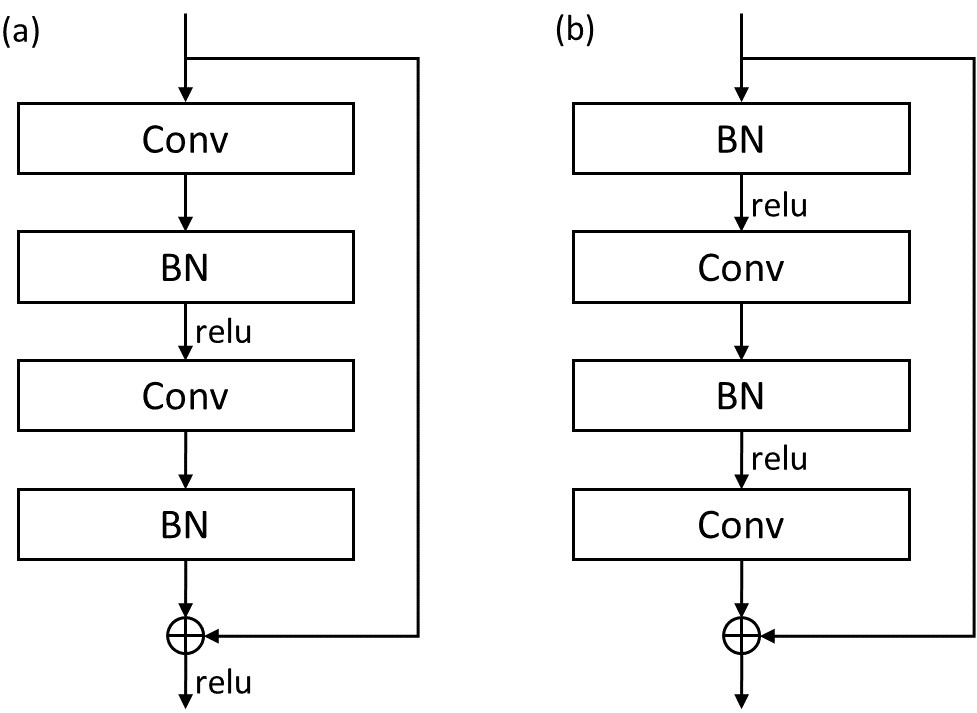
\includegraphics[width=8cm]{98_images/residual_layers.png}
\caption{(a) Aufbau des originellen Residual Layers nach \cite{deep-residual-learning}; (b) Aufbau der Weiterentwicklung eines Residual Layers \cite{identity-mappings-in-drn}.}
\label{fig:residual}
\end{figure}

\mypar Ein Jahr nach der Einführung des Residual Layers führte He et. al \cite{identity-mappings-in-drn} eine verbesserte Version ein. Ihr Aufbau ist in Abbildung \ref{fig:residual}(b) aufgezeigt. Hiermit wurde der Fehler auf den CIFAR-10-Datensatz, welches aus 60.000 Bilder aus 10 Klassen besteht \cite{krizhevsky2009learning}, von 7,61\% auf 4,92\% verringert. \cite{identity-mappings-in-drn}


% Bottleneck Layer
\subsubsection{Bottleneck Layer}
Das Bottleneck Layer (siehe Abbildung \ref{fig:bottleneck}) ist die nächste Entwicklung des ursprünglichen Residual Layers und besteht aus drei hintereinanderliegenden Convolutional Layer mit Filtern der Größen $1\times1$, $3\times3$ und $1\times1$. Die Schichten mit den $1\times1$ Filtern reduzieren erst und erhöhen dann die Dimensionen, somit hat die mittlere Schicht mit dem $3\times3$ Filter eine kleinere Ein- und Ausgangsdimension. Dieser Aufbau erinnert an einem Flaschenhals (engl. Bottleneck), woran der Name des Filters angelehnt ist. Die parameterfreie Verzweigung, die an den zwei Enden mit den höchsten Dimensionen verbunden ist, führt außerdem zu einem geringeren Zeitverbrauch. \cite{deep-residual-learning}

\begin{figure}[h!]
\centering
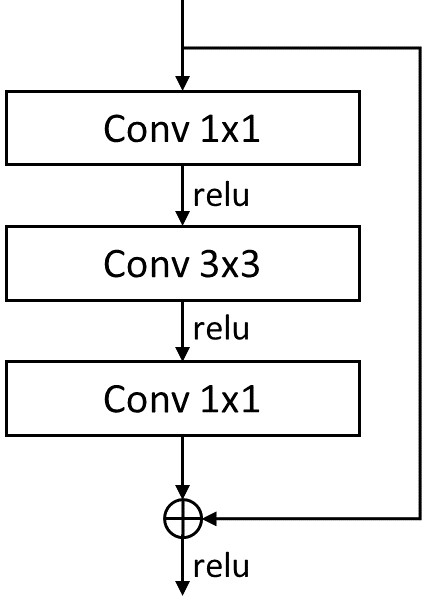
\includegraphics[width=3.5cm]{98_images/bottleneck_layer.png}
\caption{Aufbau eines Bottleneck Layers nach \cite{deep-residual-learning}.}
\label{fig:bottleneck}
\end{figure}


% Inverted Residual Layer
\subsubsection{Inverted Residual Layer}\label{inv-res-layer-section}
Ein Inverted Residual Layer, auch MBConv Layer genannt, besteht aus einer $1\times1$ Convolution, einer $3\times3$ Depthwise Convolution (kurz DepthConv), einer weiteren 1x1 Convolution und einer Shortcut-Verbindung vom Eingang des Layers bis zum Ausgang der zweiten $1\times1$ Convolution. In Abbildung \ref{fig:mbconv} ist dieser Aufbau zu sehen. Die Depthwise Convolution in der Mitte funktioniert ähnlich zu einer normalen Convolution. Der Unterschied liegt darin, dass der Filter auf den einzelnen Informationskanälen angewendet wird. Erst wird die Eingabe und der Filter in den Kanälen gespalten. Daraufhin wird der Filter angewendet und zuletzt werden die Ausgaben zusammengestellt. Diese Operation vermindert die Anzahl an Parametern. \cite{mobilenetv2}

\begin{figure}[h!]
\centering
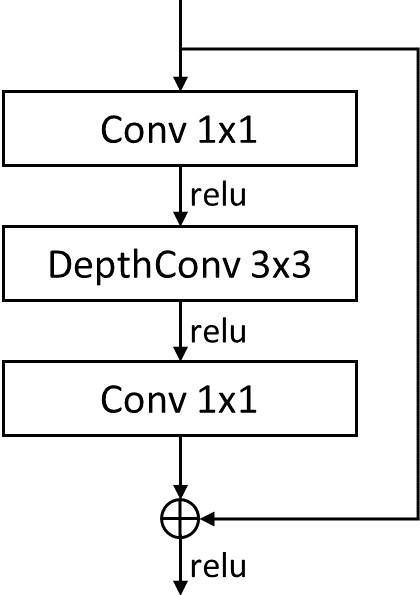
\includegraphics[width=3.5cm]{98_images/inverted_residual_layer.png}
\caption{Zusammenstellung des Inverted Residual Layer \cite{mobilenetv2}.}
\label{fig:mbconv}
\end{figure}



%
% 2.3.3 CNN Architekturen
%
\section{Netzwerkarchitekturen}\label{sec:architekturen-grundlagen}
Seit der Einführung von CNNs wurden viele unterschiedliche Architekturen für diverse Zwecke entworfen. Somit ist im Laufe der Zeit die Komplexität, aber auch die Leistung gestiegen. Dies ist am Beispiel von ImageNet ersichtlich. ImageNet ist ein Datensatz bestehend aus 14.197.122 annotierten Bildern aus unterschiedlichen Kategorien. In den letzten zehn Jahren ist die Genauigkeit des Modells mit dem besten Ergebnis von 50,9\% auf 90,2\% gestiegen (siehe Abbildung \ref{fig:imagenet}) \cite{imagenet-leaderboard}. Im Folgenden werden einige der in den letzten Jahren entworfenen Architekturen nach deren Veröffentlichungsjahr aufgezeigt.

\begin{figure}[h!]
\centering
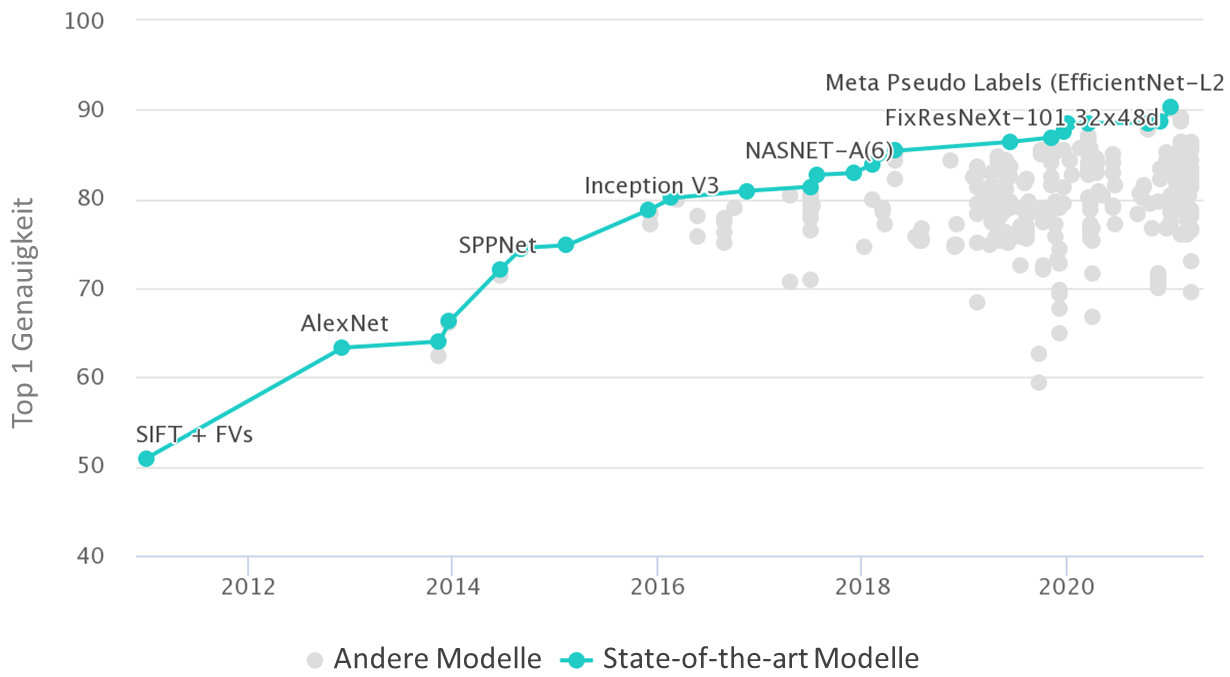
\includegraphics[width=14cm]{98_images/imagenet.png}
\caption{Rangliste für Modellergebnisse auf ImageNet über die Zeit \cite{imagenet-leaderboard}.}
\label{fig:imagenet}
\end{figure}


% AlexNet
\subsection{AlexNet}
Die von Krizhevsky et al. \cite{imagenet-class-w-deep-cnns} entworfene AlexNet-Architektur ist ein tieferes und breiteres Modell als das von LeCun \cite{lenet-2} veröffentlichte LeNet-5 CNN. AlexNet erreichte 2012 den State of the Art bei der Erkennungsgenauigkeit von Bildern und stellte einen Durchbruch in den Bereichen des Maschinellen Lernens und der Computer Vision dar \cite {the-history-began-from-alexnet}.


% VGG
\subsection{VGG}\label{sec:vgg-sec}
Das Visual Geometry Group (VGG) wurde von der Arbeitsgruppe, die diesen Namen an der University of Oxford trägt, entworfen. Es ist eine Weiterentwicklung des AlexNet und ist nach den gleichen Prinzipien aufgebaut, wie die Netze aus Ciresan et al. \cite{fleixble-hp-cnns-for-image-classification} und Krizhevsky et al. \cite{imagenet-class-w-deep-cnns}. Die zwei Varianten des Netzes, das VGG16 und das VGG19 unterscheiden sich in der Anzahl an enthaltenen Convolutional Layern, also in der Tiefe des faltenden neuronalen Netzes. Hierbei steht die Zahl am Ende der Namen für die Anzahl an Schichten mit Parametern, die Teil der Architekturen sind. \cite{very-deep-cnns-for-large-scale-img-recognition}

\mypar Ein großer Unterschied zu den neuronalen Netzen die bis 2013 den State of the Art repräsentierten, ist die Größe des Filters im ersten Convolutional Layer. Im Gegensatz zu den Filtern der Größe $11\times11$ mit einem Stride von vier in \cite{imagenet-class-w-deep-cnns}, wird im gesamten Netz eine $3\times3$ Größe mit Stride eins bevorzugt.

\mypar Laut Krizhevsky et al. \cite{very-deep-cnns-for-large-scale-img-recognition} besitzen zwei der $3\times3$ Convolutional Layer ein effektiveres Empfangsfeld als das eines $5\times5$ Layers; drei dieser Schichten besitzen das Empfangsfeld einer $7\times7$ Schicht, wie in \cite{visualizing-and-understanding-cnns}. Dies führt zu einer starken Reduzierung der Anzahl an Parametern. Für einen Stapel mit drei Convolutional Layern mit Filtern der Größe $3\times3$ mit $C$ Informationskanälen ergeben sich

\begin{equation}\label{eq:vgg1}
3(3^2C^2)=27C^2
\end{equation}

Parameter. Im Vergleich dazu, beträgt die Anzahl an Parametern bei nur einer Schicht mit $7\times7$ Filtern

\begin{equation}\label{eq:vgg2}
7^2C^2=49C^2.
\end{equation}


% ResNet
\subsection{ResNet}
Seit der Einführung der AlexNet-Architektur gehen neue neuronale Netze immer tiefer. So stieg die Anzahl an enthaltenen Convolutional Layern im Laufe der Jahre. 2012 hatte AlexNet \cite{imagenet-class-w-deep-cnns} fünf Convolutional Layer, drei Jahre später ist die Anzahl auf 16 mit dem VGG \cite{very-deep-cnns-for-large-scale-img-recognition} gestiegen.

\mypar Um eine Erhöhung der Tiefe des Netzes zu erzielen, ist es allerdings nicht ausreichend, weitere Schichten aufeinander zu stapeln. Bei tiefen Netzen tritt nämlich das sogenannte verschwindende Gradientenproblem \cite{drn-and-weight-initialization} auf, weshalb sie schwieriger zu trainieren sind. Der Gradient wird auf frühere Schichten zurück propagiert und kann, infolge wiederholten Multiplikationen, unendlich klein werden. Da das Netz tiefer und tiefer geht, wird dessen Leistung gesättigt oder nimmt schnell ab. Dies ist anhand des Beispiels aus Abbildung \ref{fig:error_deeper_networks} ersichtlich, bei dem das tiefere der beiden Netze eine schlechtere Leistung auf dem CIFAR-10-Datensatz erbrachte. 

\begin{figure}[h!]
\centering
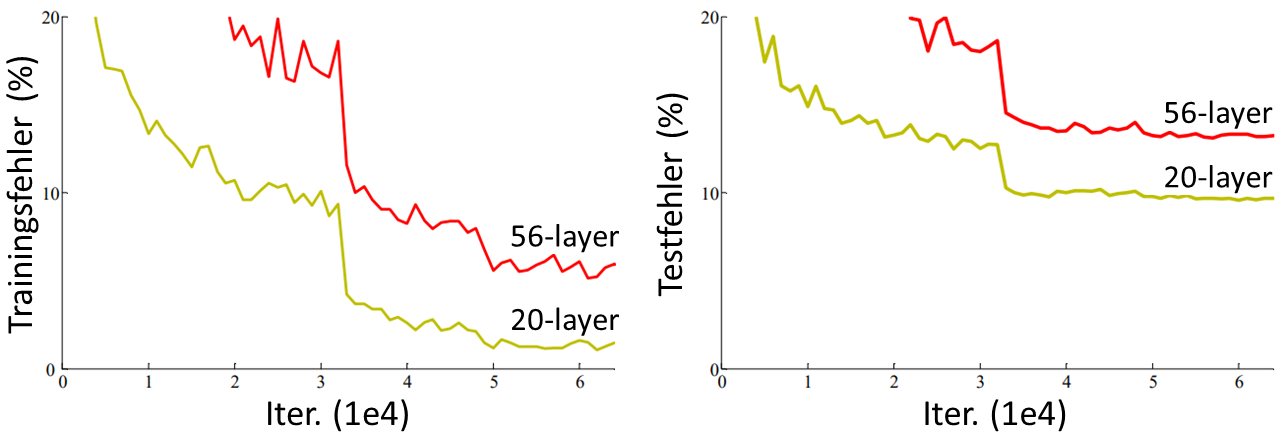
\includegraphics[width=12cm]{98_images/deeper_networks_example.png}
\caption{Trainingsfehler (links) und Testfehler (rechts) auf dem CIFAR-10-Datensatz mit ''einfachen'' Netzen mit 20 und 56 Schichten. Entnommen und Beschriftung übersetzt aus \cite{deep-residual-learning}.}
\label{fig:error_deeper_networks}
\end{figure}

\mypar Um dieses Problem zu beseitigen, werden Identitätsverknüpfungsverbindungen im Residual Layer eingeführt. Diese Schichten gelten als grundlegende Bausteine der Residual Networks, oder ResNets. Die Resnet50 und ResNet101 Architekturen nutzen das Bottleneck Layer, welches eine Weiterentwicklung des Residual Layers ist. \cite{deep-residual-learning}


% Inception-v4
\subsection{Inception-v4}
Inception-v4 \cite{inception-inceptionresnet-and-the-impact-of-residual-connections-on-learning} ist die vierte Generation der von Google entworfenen Inception-Architektur. Das Inception Layer wurde zum ersten Mal 2014 von Szegedy et al. \cite{going-deeper-with-convolutions} mit Inception-v1, oder GoogLeNet als Huldigung an Yann LeCuns LeNet-5 \cite{lenet-2}, eingeführt. In diesem Jahr gewann diese Architektur die Large Scale Visual Recognition Challenge (kurz: ILSVRC2014). Inception-v2 \cite{rethinking-inception-for-computer-vision} implentierte Batch Normalization und erzetzte die $5\times5$ Convolutional Layern durch zwei $3\times3$ Schichten, um die Anzahl an Parametern zu reduzieren. In der gleichen Veröffentlichung wurde ebenfalls die Inception-v3-Architektur \cite{rethinking-inception-for-computer-vision} eingeführt.

\mypar Die Prämisse für Inception-v4 ist das Erschaffen einheitlicherer Module. Zudem waren einige Module der früheren Entwicklung komplizierter als nötig. Hierfür wurde der ''Stem'', welcher die Operation vor den Inception-Blöcken darstellt, verändert. Zudem wurden die drei Hauptmodule Inception-A, -B und -C aktualisiert und es wurden sogenannte ''grid-reduction'' Module eingeführt, um die Breite und Höhe des Gitters zu verändern. \cite{inception-inceptionresnet-and-the-impact-of-residual-connections-on-learning}


% Inception-ResNet-v2
\subsection{Inception-ResNet-v2}
Inception-ResNet-v2 ist ein Convolutional Neural Network, welches auf der Inception-Architektur basiert und die Identitätsverknüpfungsverbindung der ResNets einbaut. Um dies umzusetzen, müssen Ein- und Ausgang nach der Convolution von der gleichen Dimension sein. Dafür werden Convolutional Layer mit Filtern der Größe $1\times1$ nach den ursprünglichen Convolutions eingesetzt. In den Inception-ResNet-A, -B und -C Modulen wird das Pooling Layer durch den Shortcut ersetzt. \cite{inception-inceptionresnet-and-the-impact-of-residual-connections-on-learning}


% Xception
\subsection{Xception}
Die 2017 veröffentliche-Xception Architektur ist von der Inception-Architektur \cite{rethinking-inception-for-computer-vision} inspiriert worden. Ein wichtiger Bestandteil von Xception ist die Einführung des Separable Convolution Layer. Der Aufbau von Xception besteht aus drei grundlegenden Teilen; dem Eingang, dem mittleren Durchfluss, welcher acht Mal wiederholt wird, und dem Ausgang. \cite{xception-dl-with-depthwise-sep-conv}


% MobileNetV3
\subsection{MobileNetV3}
MobileNetV3 ist eine Weiterentwicklung des MobileNet aus \cite{mobilenets} und wurde für die Benutzung mit CPUs von Mobiltelefonen entworfen. Das neuronale Netz besteht aus mehreren Inverted Residual Layern (siehe Abschnitt \ref{inv-res-layer-section})  und führt eine neue Aktivierungsfunktion, ''h-swish'', ein. \cite{searching-for-mobilenetv3}

\begin{equation}\label{eq:swish}
f(x)=x \cdot \sigma(\beta x), \text{         mit } \sigma(z)= \frac{1}{1+e^{-z}}
\end{equation}

\mypar Die ursprüngliche Swish-Funktion wurde 2017 von Ramachandran et al. \cite{searching-for-act-functions} eingeführt und ist in Gleichung \ref{eq:swish} beschrieben. Hierbei ist $\beta$ ein änderbarer Parameter. Laut \cite{searching-for-mobilenetv3} stellt h-swish eine Verbesserung der ursprünglichen Swish-Funktion dar, da die Rechenzeit verringert wird. Diese wird in Formel \ref{eq:h-swish} aufgezeigt.

\begin{equation}\label{eq:h-swish}
\text{h-swish}(x)=x\frac{\text{min}(\text{max}(x+3, 0), 6)}{6}
\end{equation}


% EfficientNet
\subsection{EfficientNet}
Die Grundidee hinter der Architektur von EfficientNets ist das sogenannte Compound Scaling. Anstatt Netze anhand der Tiefe (Anzahl der Schichten), Breite (Anzahl der Informationskanäle) oder Bildgröße zu skalieren, werden alle drei Dimensionen so verändert, dass sie ein Gleichgewicht bilden. Somit kann eine bessere Genauigkeit und Effizienz bei den neuronalen Netzen erzielt werden. Diese Methode kann auch bei anderen Architekturen angewendet werden. So wurde gezeigt, dass das Compound Scaling bei MobileNetV1, MobileNetV2 und ResNet-50 zu besseren Ergebnissen auf dem Imagenet-Datensatz führte. \cite{efficientnet}

\begin{equation}\label{eq:compound-scaling}
\begin{aligned}
\text{Tiefe: } d = \alpha^{\phi} \\
\text{Breite: } w = \beta^{\phi} \\
\text{Auflösung: } r = \gamma^{\phi} \\
\text{$\forall$ } \alpha \cdot \beta^2 \cdot \gamma^2 \approx 2, \alpha \geqslant 1, \beta \geqslant 1, \gamma \geqslant 1
\end{aligned}
\end{equation}

\mypar Compound Scaling verwendet einen Koeffizienten $\phi$, um die Breite, Tiefe und Auflösung gemeinsam zu bestimmen. Die Gleichungen aus \ref{eq:compound-scaling} beschreiben die skalierten Attribute. Der benutzerdefinierte Parameter $\phi$ bestimmt die zusätzlichen verfügbaren Ressourcen und $\alpha$, $\beta$ und $\gamma$ bestimmen die Verteilung dieser Ressourcen über der Tiefe $d$, Breite $w$ und Auflösung $r$. 

\begin{figure}[h!]
\centering
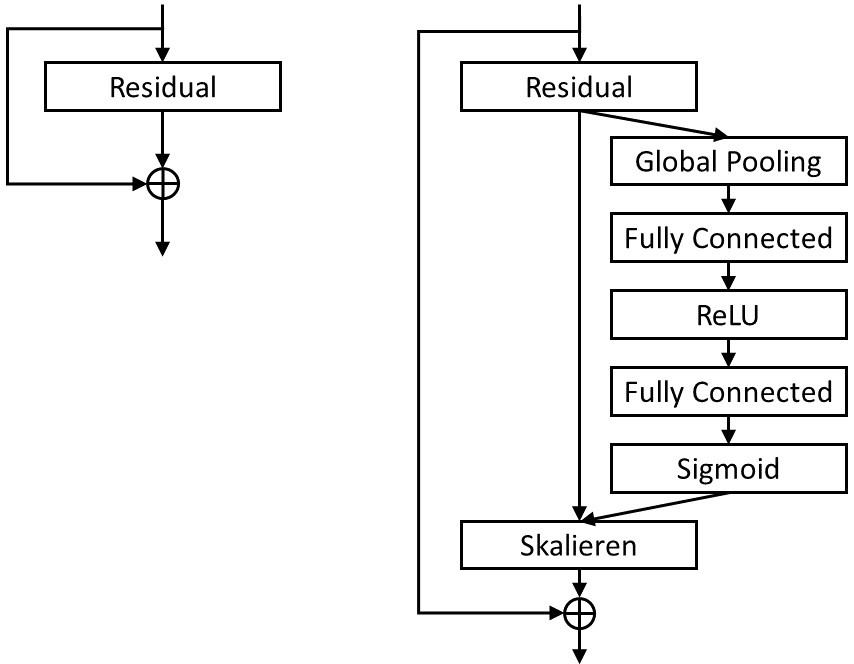
\includegraphics[width=10cm]{98_images/se_block.png}
\caption{Aufbau eines Residual Layers (links) und dem SE-ResNet Modul (rechts) nach \cite{squeeze-and-excitation-networks}.}
\label{fig:se-block-architecture}
\end{figure}

\mypar Der Hauptbaustein des EfficientNet ist das Inverted Residual Layer, welches zusätzlich noch durch Squeeze-and-Excitation (SE) optimiert wird \cite{efficientnet}. Der SE-Block besitzt am Eingang eine Convolution. Mithilfe des Poolings wird jeder Informationskanal auf einen einzigen Wert zusammengepresst. Das darauffolgende Fully Connected Layer mit einer ReLU als Aktivierungsfunktion fügt eine Nichtlinearität ein und das zweite Fully Connected Layer glättet die Funktion. Dieses Layer verwendet die Sigmoid-Funktion. Am Ende wird jede Feature Map der Faltungsoperation anhand des Ergebnisses der hinzugefügten Schichten skaliert. Abbildung \ref{fig:se-block-architecture} zeigt die Umsetzung für ein Residual Layer. Diese zusätzliche Struktur benötigt unter 1{\%} an zusätzlicher Rechenleistung und kann zu jedem neuronalen Netzwerk hinzugefügt werden. \cite{squeeze-and-excitation-networks}















    \cleardoublepage
    
     \chapter{Verwandte Arbeiten}
    \label{ch:state-of-the-art}
		% verwandte Arbeiten
Bisher wurde kein vollautomatisertes System zur geometrischen Überprüfung der Stentstruktur konzipiert. In diesem Kapitel wird an erster Stelle die Forschung im Bereich der bildbasierten Analyse von Geflechten vorgestellt. Darauffolgend wird auf den aktuellen Stand der automatisierten Inspektion von Stents eingegangen, welche größtenteils auf Verfahren der Bildverarbeitung basiert. Im Anschluss wird auf das Projekt Stents4Tomorrow \cite{flechtmaschine} eingegangen und der bisherige Fortschritt erläutert.


% Bildbasierte Analyse von Geflechten
\section{Bildbasierte Analyse von Geflechten}
Die bildbasierte Analyse von Geflechten wurde bereits von mehrfachen Studien untersucht, was zu diversen Lösungsansätzen geführt hat. So basieren die von Phoenix \cite{phoenix1978mechanical}, Zhang et al. \cite{zhang1999analysis} und Guyader et al. \cite{guyader2013analysis} entworfenen Systeme auf geometrische Beziehungen im Geflecht. Die von Alpyildiz \cite{alpyildiz20123d} veröffentlichte Arbeit schlägt dreidimensionale Garnwege im Geflecht vor, welche für die Simulation der Geflechtgeometrie notwendig sind. Darüber hinaus entwickelten Hunt et al. \cite{hunt2019machine} ein Computer-Vision-System für die Echtzeitvermessung des Flechtwinkels in der Produktion. Das System verwendet eine 2D diskrete Fourier-Transformation für die Verarbeitung der Bilder und erzielt eine Genauigkeit von $\pm$1-2 Grad bei der Vermessung von einzelnen Winkeln. \cite{hunt2019machine} Liu et al. \cite{liu2019automatic} implementierten ein ähnliches System unter der Verwendung des Canny-Algorithmus \cite{canny1986computational} und der Hough-Transformation \cite{duda1972use}.

\mypar Xiao et al. untersuchten die Vermessung der Picklänge und des Flechtwinkels mit unterschiedlichen Ansätzen in mehreren Studien. Beim ersten Ansatz \cite{xiao2018measurement} wurden vielfältige Kantendetektoren eingesetzt, um die Ecken im Bild zu ermitteln. Diese Herangehensweise wurde darauffolgend in \cite{xiao2019surface} durch die Einführung des ''local edge extreme''-Algorithmus ersetzt. In einer weiteren Veröffentlichung \cite{pei2019surface} wurde für die Vermessung der oben genannten Größen eine auf die sogenannte ''gray projection'' basierte Methode eingeführt, mit der eine hohe Genauigkeit erzielt wurde. Darüber hinaus wurde ein Faster R-CNN-Modell in \cite{xiao2020surface} trainiert, um Picklängen und Flechtwinkel in Bildern, wie in Abbildung \ref{fig:faster_rcnn} aufgezeigt, zu lokalisieren und messen.

\begin{figure}[h!]
\centering
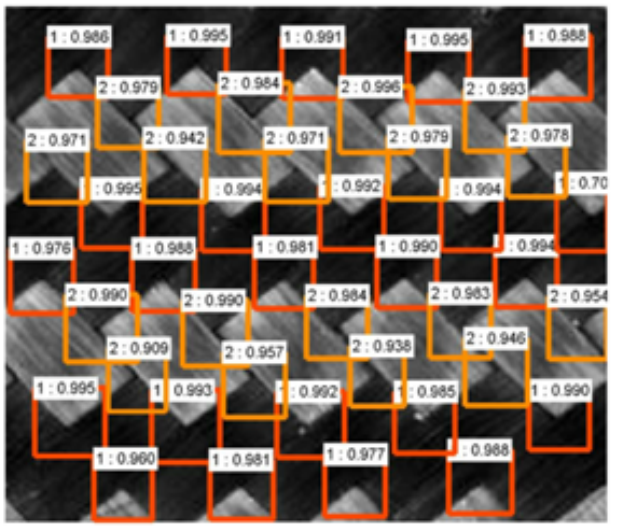
\includegraphics[width=7cm]{98_images/xiao_2020.png}
\caption{Testergebnisse der Anwendung eines Faster R-CNN auf Bilder von Geflechten. Entnommen aus \cite{xiao2020surface}.}
\label{fig:faster_rcnn}
\end{figure}


% Visuelle Inspektion von Stents
\section{Visuelle Inspektion von Stents}
Es wurden bereits einige Untersuchungen und Studien im Bereich der visuellen Inspektion von Stents durchgeführt. Eine von Farmer \cite{farmer2005automated} durchgeführte Studie führte ein Bildverarbeitungssystem ein, um die Drähte und Kanten des Stents zu untersuchen. Das System wird von zwei Sensorenpaketen betrieben. Das erste Paket wird für die Überprüfung der Drähte und Kanten verwendet, wohingegen das zweite Paket die Fläche zwischen den Drähten betrachtet. Das entworfene System verfehlte 0,08{\%} der Defekte, identifizierte 8{\%} der Defekte falsch positiv und konnte mit einer Geschwindigkeit von 18 mm pro Minute und sechs Sekunden betrieben werden. \cite{farmer2005automated}

\mypar In der von Ibraheem und Binder \cite{ibraheem2009automated} veröffentlichten Arbeit, wird eine Zeilenkamera verwendet, um ein hochauflösendes Bild des gesamten Stents aufzunehmen. Zur Erkennung von Fehlern werden unterschiedliche Verfahren aus der Kantendetektion und Bildsegmentierung angewendet. Somit werden bogenförmige Segmente an den Kreisbögen des Stents im Bild angepasst. Anhand dieser Anpassung können die Mittelpunkte und Radien der Bögen bestimmt werden. Aus den Abweichungen zwischen den Werten können lokale Fehler detektiert werden. \cite{ibraheem2009automated}

\begin{figure}[h!]
\centering
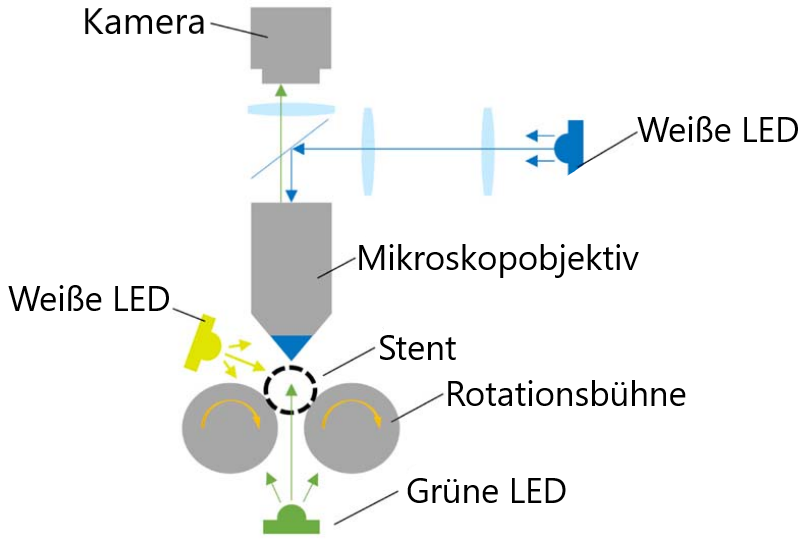
\includegraphics[width=7cm]{98_images/aufbau_bermudez.png}
\caption{Aufbau des von Bermudez et al. 2016 entworfenen Systems mit einem dreifachen Beleuchtungssystem. Entnommen und übersetzt aus \cite{bermudez2017stent}.}
\label{fig:bermudez_aufbau}
\end{figure}

\mypar In einer von Bermudez et al. \cite{bermudez2017stent} durchgeführten Studie werden Bilder, wie in Abbildung \ref{fig:bermudez_aufbau} zu sehen, mithilfe einer Mikroskopanordnung, einem dreifachen Beleuchtungssystem und einer Rotationsbühne aufgenommen. Anhand einer Segmentierung kann der Draht des Stents vom Hintergrund des Bildes isoliert werden (siehe Abbildung \ref{fig:bermudez_stent_mask}). Durch die Anwendung morphologischer Operatoren wird das segmentierte Bild weiterverarbeitet, um Kanten sichtbar zu machen. Im Anschluss werden die Drahtbreite und Kantenrundheit auf geometrische Fehler untersucht \cite{bermudez2017stent}. Eine weitere Veröffentlichung stellte ein verbessertes System mit einem verbesserten Vermessungssystem vor. Hierfür werden sogenannte Confocal und Coherence Scanning Interferometry (kurz CSI \cite{de2011coherence}) angewendet, um die Form, Textur und Defekte der Oberfläche von Stents anhand von 3D-Messtechnik evaluieren zu können \cite{bermudez2017optical}. Des Weiteren wird in einer darauffolgenden Studie ein Klassifikator eingeführt, welcher Defekte von Stents an der Oberfläche oder Kanten in unterschiedliche Arten einstufen kann \cite{bermudez2017automated}.

\begin{figure}[h!]
\centering
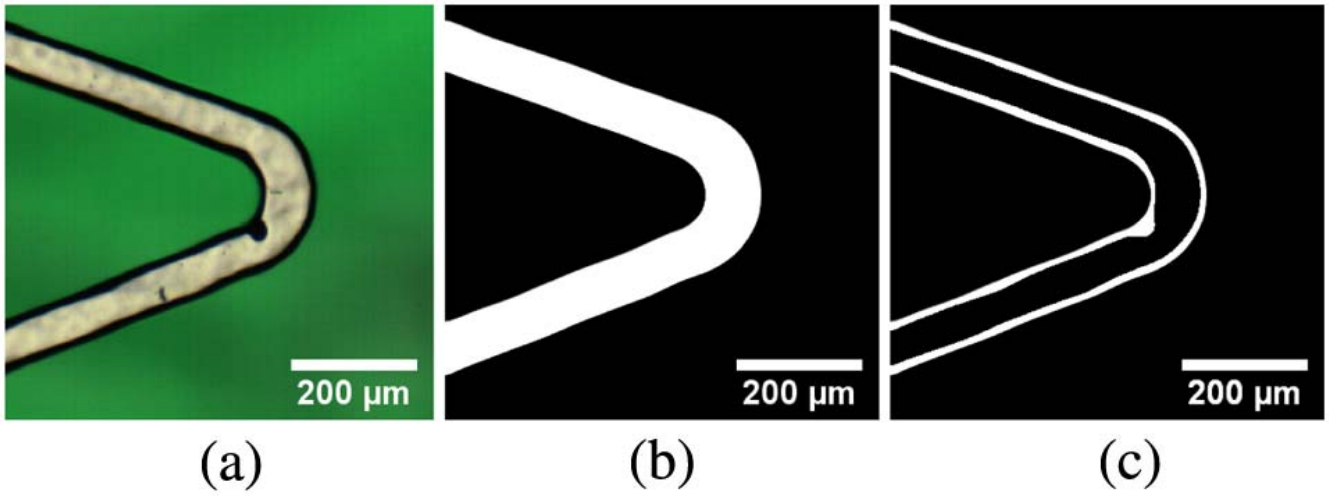
\includegraphics[width=10cm]{98_images/stent_edge_mask.png}
\caption{Stent mit einem Rissdefekt: (a) ursprüngliches Bild, (b) Maske der Oberfläche, (c) Maske der Kanten. Entnommen aus \cite{bermudez2017stent}.}
\label{fig:bermudez_stent_mask}
\end{figure}


% Stents4Tomorrow
\section{Stents4Tomorrow}
Im Rahmen des Stents4Tomorrow-Projekts \cite{flechtmaschine} soll der Prozess der visuellen Inspektion von Stents während der Produktion automatisieren. Ein wichtiger Bestandteil ist die Erkennung von Fehlern im Geflecht. Houssem \cite{houssem} setzte sich sowohl mit der Berechnung des Flechtwinkels als auch mit der Erkennung von Unregelmäßigkeiten im Flechtmuster auseinander. Ähnlich wie in \cite{hunt2019machine} wurden die Hough- und 2D diskrete Fourier-Transformation angewendet und miteinander verglichen. Hierbei führte die zweidimensionale diskrete Fourier-Transformation zu besseren Ergebnissen bei Bildern aller Flechtwinkel. Zur Überprüfung des Flechtmusters wurde die U-Net-Architektur implementiert und mit einem Convolutional Autoencoder verglichen. U-Net zeigte eine höhere Leistung vor. \cite{houssem}

\mypar Zusammen mit dem Flechtwinkel ist die Picklänge ein wichtiger Bestandteil der Geometrie von Stents. Aus diesem Grund untersuchte Schorle \cite{felix} die Vermessung der Picklänge anhand unterschiedlicher Methoden. Durch die Anwendung faltender neuronaler Netze konnte eine Genauigkeit von 0,267 Millimetern bei der Vermessung der durchschnittlichen Länge von Picks auf einer Linie erreicht werden. \cite{felix}

\mypar Neben der zuverlässigen Fehlererkennung im Stent ist die Effizienz des Systems bei der Korrektur der erkannten Fehler wichtig. Djamal \cite{aulia} setzte sich mit der Optimierung dieses Vorgangs auseinander. Somit wurden sechs Abläufe zur Fehlerkorrektur entworfen. Bei den zwei nicht-optimierten Vorgängen wurden zwei optimale Ansätze gefunden. Zudem konnte eine optimale Lösung für die Genauigkeit und für die Ablaufzeit konzipiert werden. \cite{aulia}

\mypar Der Grundbestandteil der Fehlerkorrektur ist das entsprechende System, um diese auszuführen. In \cite{valentin} wird das Konzept eines kamerabasierten Korrektursystems zur Verbesserung des Flechtprozesses von Stents vorgestellt. Die Funktionsweise des Algorithmus des Systems ist hierbei in drei grundlegende Schritte aufgeteilt: Erst wird die Picklänge vermessen, darauffolgend wird über die Korrektur entschieden und im Anschluss wird diese spezifiziert. Das vorgestellte System zeichnet sich durch die Verwendung mehrerer arbeitsteiliger Convolutional Neural Networks aus. Diese sind in einer Programmlogik miteinander verknüpft, sodass Messfehler besser eingegrenzt werden können. \cite{valentin}
    \cleardoublepage

	\chapter{Konzept}
	\label{ch:Konzept}  	
		% Einleitung
Im folgenden Kapitel wird der grundlegende Aufbau dieser Arbeit vorgestellt und die im Rahmen dieser Arbeit relevanten Schritte hervorgehoben. Außerdem wird das Verfahren zur Berechnung der Picklänge erläutert und auf die Auswahl der Netzwerkarchitekturen und das Erfassen der Bilddaten eingegangen.

\begin{figure}[h!]
\centering
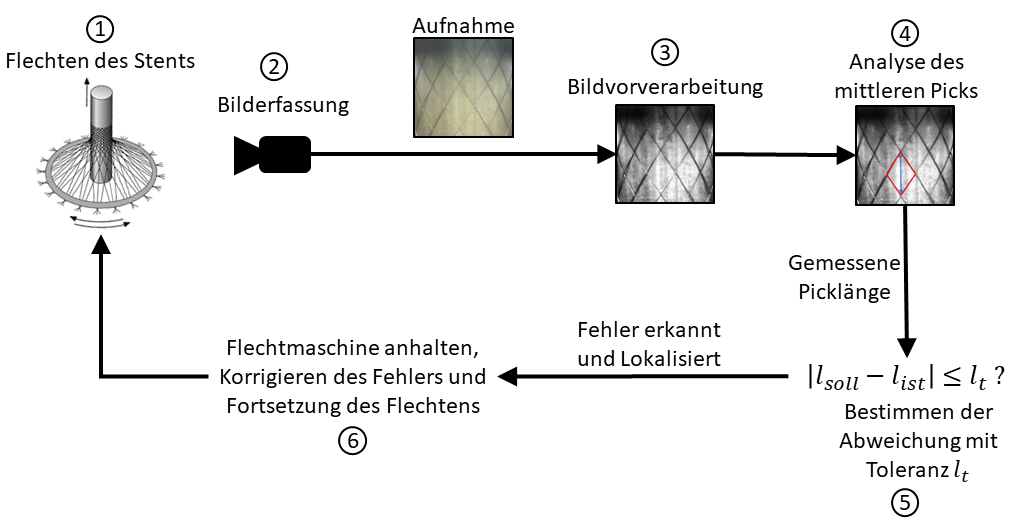
\includegraphics[width=15cm]{98_images/aufbau_projekt.png}
\caption{Aufbau des Gesamtsystems zur automatisierten Fehlererkennung und -korrektur von Stents basierend auf Kamerabildern}
\label{fig:aufbau_des_projekts}
\end{figure}


% Aufbau des Projekts
\section{Aufbau des Projekts}\label{sec:?}
Der grundlegende Aufbau des Systems für die automatische Fehlererkennung von Stents in der Produktion ist in Abbildung \ref{fig:aufbau_des_projekts} aufgezeigt. Die Stents werden bei einen vorgegebenen Flechtwinkel von einer Flechtmaschine hergestellt. Der Verlauf dieses Prozesses soll mit einer Kamera überwacht werden. Nach einer Vorverarbeitung der Bilder wird die Picklänge des mittleren Picks bestimmt und anhand der gewünschten Länge die Abweichung zwischen diesen zwei Werten berechnet. Mittels eines festgelegten Toleranzwertes wird entschieden, ob ein Fehler vorliegt oder nicht. Sollte ein Fehler im Geflecht vorhanden sein, wird die Flechtmaschine angehalten, der Defekt korrigiert und das Flechten im Anschluss fortgesetzt. Im Rahmen dieser Arbeit wurden drei dieser Schritte betrachtet: die Bildvorverarbeitung der Aufnahmen, deren Analyse, um die Länge des mittleren Picks zu bestimmen und die Bestimmung der Abweichung der Netzausgaben.


% Berechnung der Picklänge
\section{Berechnung der Picklänge}
Es gibt mehrere Ansätze, mit denen eine Pickanalyse durchgeführt werden kann. Schorle \cite{felix} untersuchte Methoden der Bildverarbeitung des klassischen maschinellen Lernens und faltende neuronale Netze, um den Mittelwert der Längen aller Picks in der Mitte des Bildes zu vermessen. Wie in Abbildung \ref{fig:abweichungen-vgl} dargestellt, kann trotz eines korrekten Mittelwertes ein Fehler in der Struktur des Stents vorliegen. Aus diesem Grund wird in dieser Arbeit nur der sich in der Mitte des Bildes befindende Pick analysiert. Aus den in \cite{felix} untersuchten Methoden wurden mit faltenden neuronalen Netzen die besten Ergebnisse erreicht. Deshalb werden sie im Rahmen dieser Arbeit für die Vermessung der Picklänge eingesetzt.

\begin{figure}[h!]
\centering
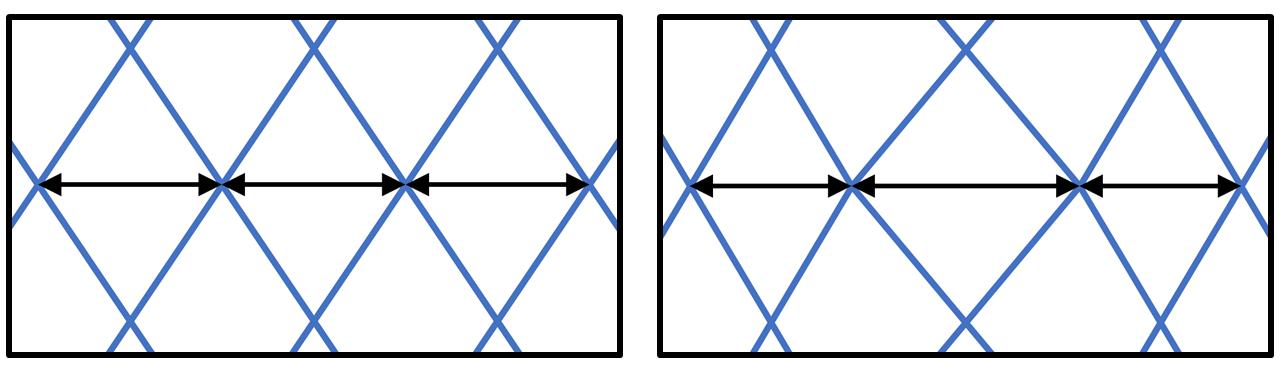
\includegraphics[width=13cm]{98_images/abweichungen_vgl.png}
\caption{Beispiel für zwei Zeilen von Picks mit gleicher durchschnittlicher Picklänge, fehlerfrei (links) und fehlerhaft (rechts)}
\label{fig:abweichungen-vgl}
\end{figure}


% Auswahl der CNNs
\section{Auswahl der faltenden neuronalen Netzen}\label{sec:auswahl-cnns}
Um möglichst vielfältige Netzwerkarchitekturen zu analysieren, wurden die in Kapitel \ref{sec:architekturen-grundlagen} beschriebenen Modelle implementiert und optimiert. Die Auswahl enthält sowohl aktuelle Architekturen wie EfficientNet, als auch Netze wie AlexNet, welche einen einfachen Aufbau haben. Zudem variieren die Einsatzgebiete der gewählten Architekturen.

\mypar Bei der Anwendung faltender neuronaler Netze mit Bildern gibt es drei große Anwendungsbereiche. Die meist verbreitete ist die Bildklassifizierung, welche Bilder in unterschiedliche Kategorien einstuft. Weiterhin wird die Objekterkennung angewendet, um beliebige Objekte innerhalb eines Bildes mit einem sogenannten Begrenzungskasten zu erkennen und einzurahmen. Im Vergleich dazu wird bei der semantischen Segmentierung jedem Pixel eine Kategorie zugeordnet. So kann das Bild in mehrere Bereiche oder Cluster aufgeteilt werden. Einige Beispiele zu diesen Bereichen sind in Abbildung \ref{fig:cnn-anwendungen} aufgezeigt. In der Netzauswahl befinden sich Netze, die auch für weitere Anwendungen eingesetzt werden. Dazu zählen die Maschinenübersetzung, bei der Texte aus einer Sprache in eine andere umgewandelt werden können und die Superauflösung, welche sich mit der Verbessung der Auflösung von Bildern auseinandersetzt.

\begin{figure}[h!]
\centering
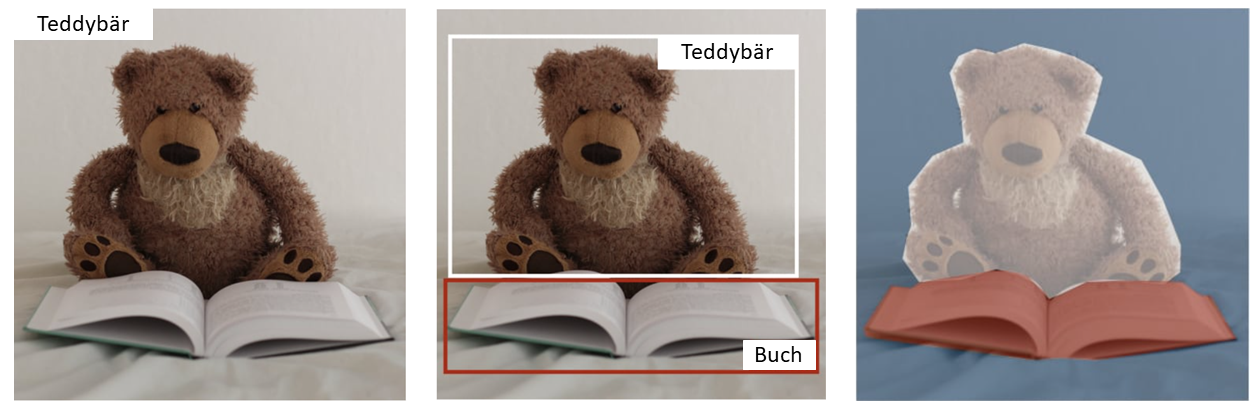
\includegraphics[width=15cm]{98_images/cnn_anwendungen.png}
\caption{Beispiele für die drei größten Anwendungsbereiche von CNNs: Klassifizierung (links), Objekterkennung (Mitte), Segmentierung (rechts). Ursprüngliche Bilder aus \cite{amidi2018convolutional}.}
\label{fig:cnn-anwendungen}
\end{figure}


% Erfassung der Trainingsdaten
\section{Erfassung der Trainingsdaten}\label{sec:erfassung-trainingsdaten}
Das Trainieren von neuronalen Netzen erfordert einen Datensatz. Hierfür wurden Bilder von Stents inklusive der zugehörigen Picklängen als Labels verwendet. Die vom Projekt Stents4Tomorrow \cite{flechtmaschine} zur Verfügung gestellten Bilder zeigen mehrere Segmente von Stents mit unterschiedlichen Flechtwinkeln. Diese Bilder der Größe $3088 \times 2064$ enthalten Informationen, wie der Hintergrund, welche für die Vermessung der Picklänge irrelevant sind. Zudem wird ein sehr langer Abschnitt des Stents gezeigt, wodurch nicht immer ein Pick in der Mitte des Bildes zu sehen ist. Aus diesem Grund wurden zur Verfügung gestellte vorgeschnittene Bilder der Größe $450 \times 450$ verwendet, um die neuronalen Netze zu trainieren. Ein Beispiel für eines der ursprünglichen Bilder und ein vorgeschnittenes Bild ist in Abbildung \ref{fig:bild_normal_vorgeschnitten} zu sehen. Als Label für die Bilder wird die Länge des mittleren Picks im Bild in Pixel angegeben.

\begin{figure}[ht!]
\centering
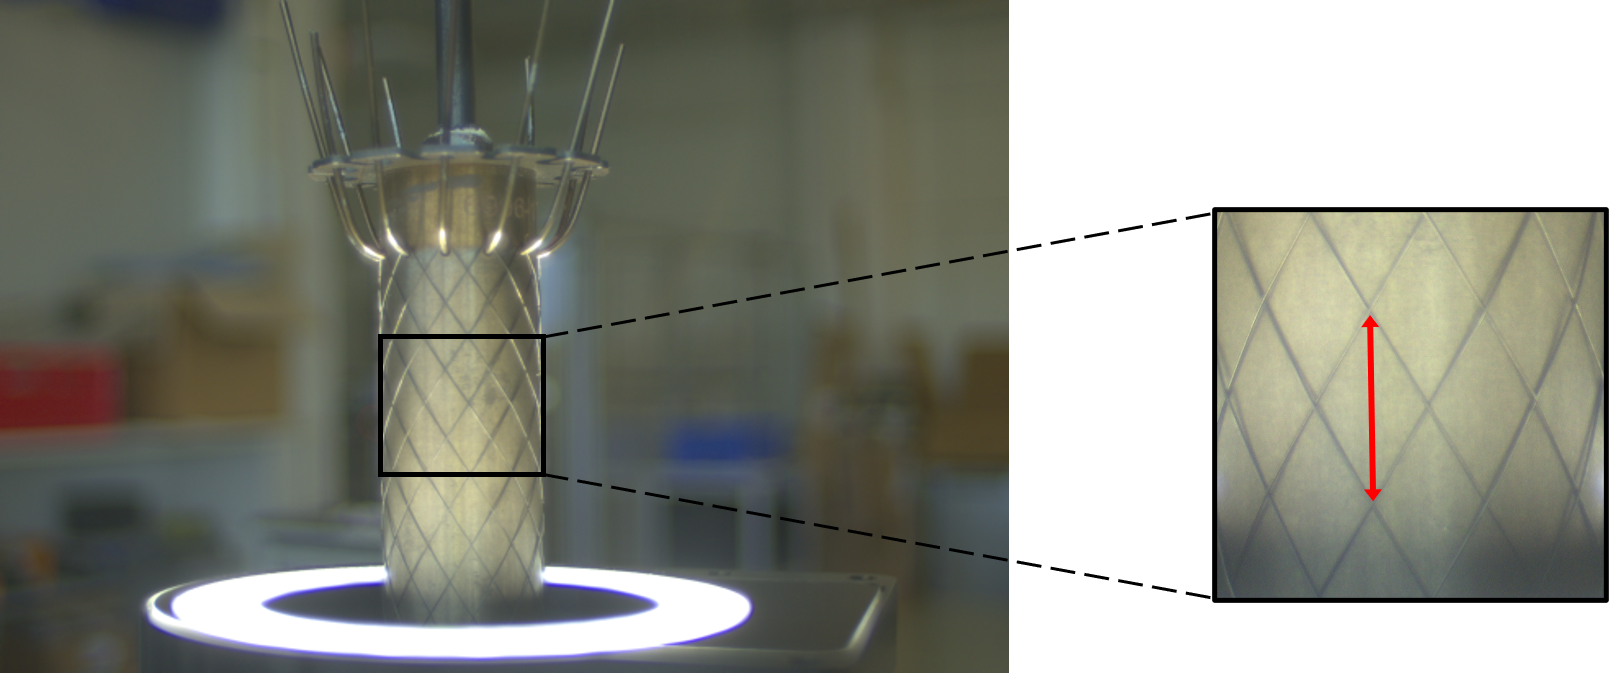
\includegraphics[width=12cm]{98_images/stent_normal_cropped.png}
\caption{Ursprüngliches Bild der Größe $3088 \times 2064$ (links) und vorgeschnittene Variante (rechts). Die Länge des sich in der Mitte des in der Bildmitte befindlichen Picks ist rot eingezeichnet.}
\label{fig:bild_normal_vorgeschnitten}
\end{figure}









    \cleardoublepage    
    
    \chapter{Implementierung}
    \label{ch:implementierung}   
   		% Einleitung
Die Realisierung der Bildvorverarbeitung, Analyse des mittleren Picks und Bestimmung der Abweichung werden im folgenden Kapitel vorgestellt. Im ersten Abschnitt wird in die Aufbereitung und Aufteilung des Datensatzes für das Trainieren und Testen der neuronalen Netze eingegangen. Darauffolgend wird auf die Implementierung der faltenden neuronalen Netze eingegangen und die Auswahl der Hyperparameter erklärt. Anschließend wird im dritten Abschnitt dieses Kapitels eine vereinfachte Form der Fehlerlokalisierung aufgebaut.


% Trainingsdaten
\section{Trainingsdaten}
Wie in Abschnitt \ref{sec:erfassung-trainingsdaten} beschrieben, wurden vorgeschnittene Bilder der Größe $450 \times 450$ verwendet; insgesamt standen 23.527 Bilder zur Verfügung. Die dazugehörigen Labels der Bilder wurden in Zusammenarbeit mithilfe eines Python-Skriptes erstellt. Hierbei wurden Bilder, bei denen der Stent nicht sichtbar war, kein Pick im Mittelpunkt lag oder sich dieser zwischen zwei Picks befand, aussortiert. Insgesamt betrifft dies 7.586 Aufnahmen. Beispiele dafür sind in Abbildung \ref{fig:datensatz-fehler-1} dargestellt. 

\begin{figure}[h!]
\centering
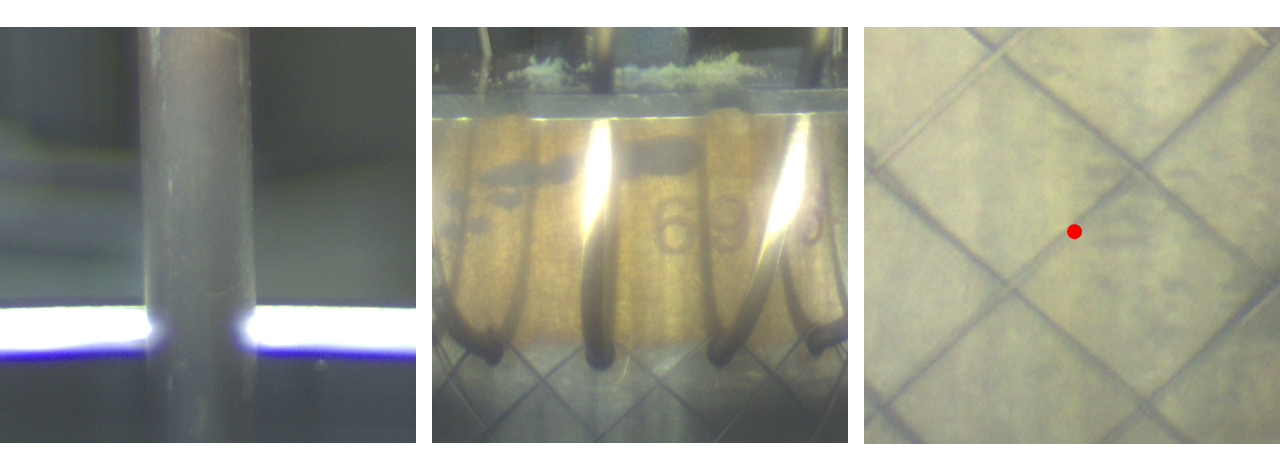
\includegraphics[width=12cm]{98_images/datensatz_bsp1.png}
\caption{Beispiele für ungeeignete Bilder für das neuronale Netz: kein Stent im Bild sichtbar (links), kein Pick in der Mitte des Bildes (Mitte), kein eindeutiger Pick in der Mitte (rot markiert) des Bildes (rechts). Bilder aus \cite{flechtmaschine} entnommen.}
\label{fig:datensatz-fehler-1}
\end{figure}

\mypar Zudem wurden im Anschluss weitere 11.150 Bilder aussortiert. Aufnahmen, bei denen die Lichtverhältnisse suboptimal waren, wurden entfernt, weil die Sichtbarkeit des mittleren Picks somit beeinflusst wurde und er nicht immer klar erkennbar war. Bilder von Stents, bei denen einer der Drähte gerissen war, wurden ebenfalls nicht übernommen. Abbildung \ref{fig:datensatz-fehler-2} zeigt drei Beispiele für die zuvor genannten Fälle. 

\begin{figure}[h!]
\centering
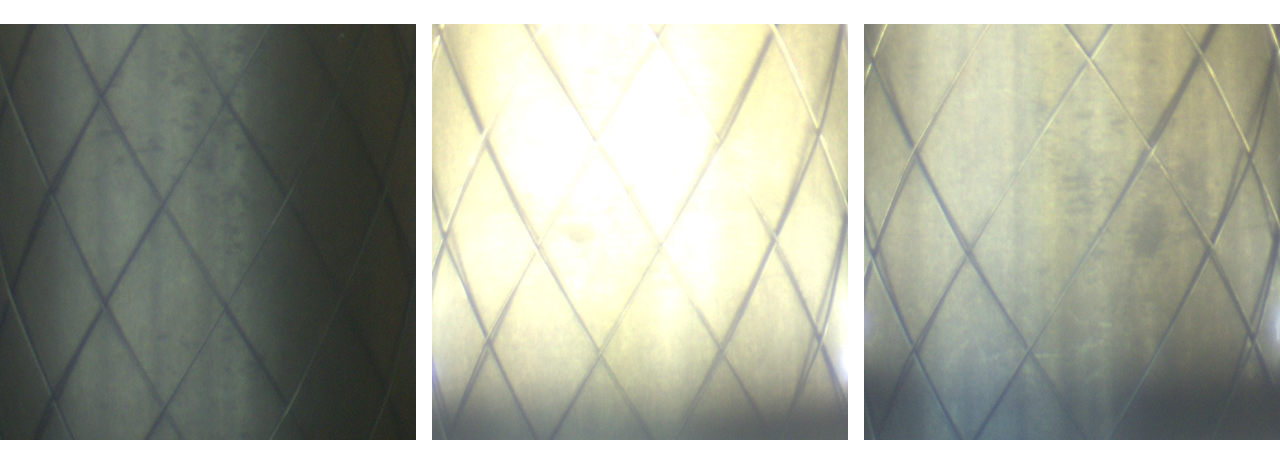
\includegraphics[width=12cm]{98_images/datensatz_bsp2.png}
\caption{Weitere Beispiele für aussortierte Bilder: ohne Licht (links), starke Lichtbestrahlung (Mitte), Draht gerissen (rechts). Bilder aus \cite{flechtmaschine} entnommen.}
\label{fig:datensatz-fehler-2}
\end{figure}

\mypar Nach dem Aussortieren ergab sich ein Datensatz mit 4.791 Bildern von Stents mit Flechtwinkeln von 30, 40, 50, 60 und 70 Grad. Tabelle \ref{Tab:Datensatz1} zeigt die Aufteilung der Anzahl an verwendbaren und aussortierten Bilddaten.

\begin{table}[h!]
\begin{center}
\begin{tabular}{cc}
Gesamte Bilder                & 23.527 \\ \hline
Ungeeignetes Licht            & 4.140  \\
Draht gerissen                & 7.010  \\
Kein Stent oder Pick sichtbar & 7.586  \\ \hline
Verwendbare Bilder            & 4.791 
\end{tabular}
\caption{Aufteilung der ursprünglichen Aufnahmen in verwendbare und ungeeignete Bilder}
\label{Tab:Datensatz1}
\end{center}
\end{table}

% Aufbereitung der Trainingsdaten
\section{Aufbereitung der Trainingsdaten}
Wie bereits beschrieben, konnten 4.791 geeignete Bilder aus den ursprünglichen Daten entnommen werden. Um den Datensatz zu erweitern, wurden diese verwendbaren Bilder durch das Drehen um 180° augmentiert. Da sich dadurch der zuvor markierte Pick aus dem Mittelpunkt des Bildes verschieben kann, wurde das Skript zum Labeln der Bilder erweitert. Somit konnten zuvor falsch gesetzte Labels gelöscht und Labels, bei denen sich der mittlere Pick nicht änderte für das augmentierte Bild übernommen werden. Hierdurch entstanden 3.892 weitere verwendbare Bilder inklusive Labels. Die Übersicht der Zusammensetzung des gesamten Datensatzes ist in Tabelle \ref{Tab:Trainingsdaten1} dargestellt.


\begin{table}[h!]
\begin{center}
\begin{tabular}{cc}
Datensatz             & Anzahl Bilder \\ \hline
Vorgeschnittene Daten & 4.791         \\
Augmentierte Daten    & 3.892         \\ \hline
Gesamter Datensatz    & 8.683        
\end{tabular}
\caption{Übersicht über die vorgeschnittenen, augmentierten und den daraus entstandenen gesamten Daten}
\label{Tab:Trainingsdaten1}
\end{center}
\end{table}

\mypar Eine detailliertere Darstellung vom Aufbau des Datensatzes wird durch Tabelle \ref{Tab:Trainingsdaten2} aufgezeigt. Es ist ersichtlich, dass keiner der Flechtwinkel einen mehrheitlichen Anteil des Datensatzes darstellt, wodurch eine Gleichverteilung der Flechtwinkel in den unterschiedlichen Datensätzen gewährleistet wird.. Im gesamten Datensatz betragen die kleinste und größte Picklänge 40,0 und 219,06 Pixel. Zudem entspricht ein Millimeter 23 Pixel in den Bildern. 

\begin{table}[h!]
\begin{center}
\begin{tabular}{l|l|l|l|l|l}
                       & 30 Grad & 40 Grad & 50 Grad & 60 Grad & 70 Grad \\ \hline
Vorgeschnittene Bilder & 880     & 1.142   & 988     & 878     & 903     \\
Augmentierte Bilder    & 816     & 974     & 845     & 657     & 600     \\ \hline
Gesamte Bilder         & 1696    & 2116    & 1833    & 1535    & 1503    \\
Prozentanteil          & 19,5    & 24,4    & 21,1    & 17,7    & 17,3   
\end{tabular}
\caption{Aufteilung der vorgeschnittenen und augmentierten Daten nach Flechtwinkel}
\label{Tab:Trainingsdaten2}
\end{center}
\end{table}


% Bildvorverarbeitung
\subsection{Bildvorverarbeitung}
Um die Erkennung gewisser Merkmale im Bild deutlicher zu machen, wurden die Bilder entsprechend vorverarbeitet. Hierfür wurde ein Histogrammausgleich durchgeführt, konkret der kontrastbegrenzte adaptive Histogrammausgleich aus Abschnitt \ref{sec:clahe-sec}. Die Implementierung wurde mit der Python-Bibliothek OpenCV \cite{bradski2000opencv} durchgeführt. Die Anwendung des gewöhnlichen Histogrammausgleichs, AHE und CLAHE aus Kapitel \ref{sec:histogramm-sec} wird in den Abbildungen \ref{fig:30grad-cropped-img}, \ref{fig:30grad-hist-eq-img}, \ref{fig:30grad-ahe-img} und \ref{fig:30grad-clahe-img} visualisiert.

\begin{figure}[ht]
\centering
\begin{minipage}[b]{0.45\linewidth}
    \centering
    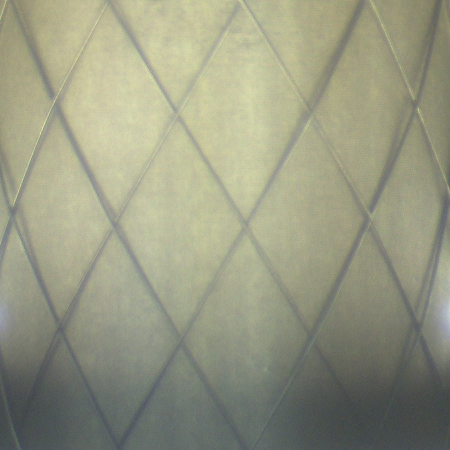
\includegraphics[width=4.5cm]{98_images/30grad_cropped.png}
    \caption{Ursprüngliches Bild}
    \label{fig:30grad-cropped-img}
\end{minipage}
\quad
\begin{minipage}[b]{0.45\linewidth}
    \centering
    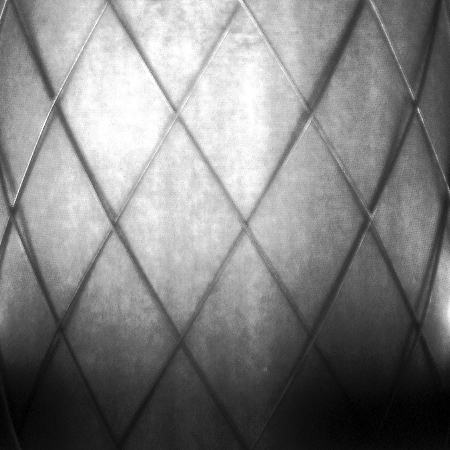
\includegraphics[width=4.5cm]{98_images/30grad_hist_eq.png}
    \caption{Histogrammausgleich}
    \label{fig:30grad-hist-eq-img}
\end{minipage}
\end{figure}

\begin{figure}[ht]
\centering
\begin{minipage}[b]{0.45\linewidth}
    \centering
    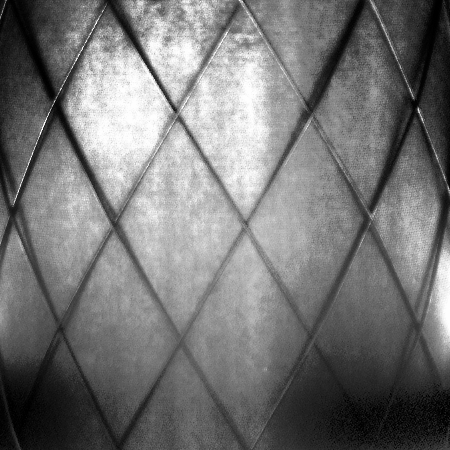
\includegraphics[width=4.5cm]{98_images/30grad_ahe.png}
    \caption{AHE}
    \label{fig:30grad-ahe-img}
\end{minipage}
\quad
\begin{minipage}[b]{0.45\linewidth}
    \centering
    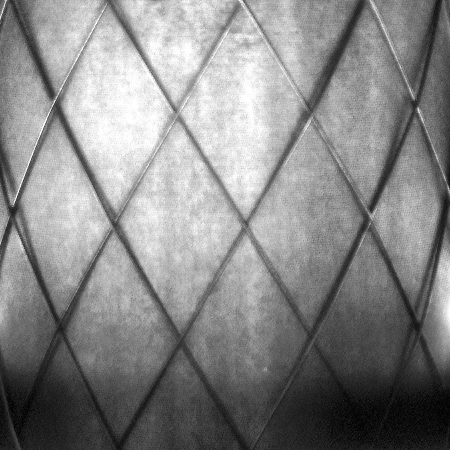
\includegraphics[width=4.5cm]{98_images/30grad_clahe.png}
    \caption{CLAHE}
    \label{fig:30grad-clahe-img}
\end{minipage}
\end{figure}


% Aufteilen und Normalisieren der Daten
\subsection{Aufteilen und Normalisieren der Daten}
Wie in Tabelle \ref{Tab:Trainingsdaten1} aufgezeigt, besteht der gesamte Datensatz aus 8.683 verwendbaren Bildern. Um die neuronalen Netze zu trainieren, werden ein Trainings- und ein Validierungsdatensatz benötigt. Zusätzlich ist ein Testdatensatz für die Evaluierung der einzelnen Netze notwendig. Aus diesem Grund wurde der Datensatz, wie in Tabelle \ref{Tab:train-val-test-tabelle} dargestellt, in drei kleinere Datensätze aufgeteilt. Dabei enthält der Trainingsdatensatz 70{\%} der Daten. Die Datensätze für die Validierung und das Testen bestehen jeweils aus 15{\%} der Bilder und Labels. 

\begin{table}[h!]
\begin{center}
\begin{tabular}{cc}
\textbf{Datensatz}   & \textbf{Anzahl Bilder} \\ \hline
Training    & 6.078         \\
Validierung & 1.302         \\
Test        & 1.303        
\end{tabular}
\caption{Aufteilung des gesamten Datensatzes in drei kleinere Datensätze}
\label{Tab:train-val-test-tabelle}
\end{center}
\end{table}

\mypar Wie in \cite{jo2019effectiveness} wurden die Daten anhand einer sogenannten Min-Max-Normalization zwischen den Werten Null und Eins gesetzt. Der MinMax-Scaler wurde erst auf den Inhalt des Trainingsdatesatzes angepasst und danach auf alle drei Datensätze angewendet. Um die Bilder und Labels aus diesen Datensätzen an die Netzwerkarchitekturen zu übergeben, wurde die Dataset API aus der Tensorflow-Bibliothek \cite{abadi2016tensorflow} verwendet, sodass eine Datenpipeline aufgebaut werden konnte.

\mypar Beim ersten Schritt wurden die Datensätze in TFRecord-Dateien umgewandelt. Dies hat den Vorteil, dass sie eine niedrigere Speicherkapazität benötigen und die Informationen der einzelnen Bilder zusammen mit ihren zugehörigen Labels hinterlegt werden. Zudem ist somit eine ununterbrochene Verbindung zum Laufwerk, auf dem die gesamten Daten gespeichert sind, nicht notwendig.

\mypar Um die Daten an den neuronalen Netzen zu übergeben, werden die einzelnen TFRecord-Dateien eingelesen. Mittels der Dataset API werden die eingelesenen Daten in einen Datensatz überführt. Danach werden die Bilder dekodiert und gecastet, um auf den Datentyp float32 umgewandelt zu werden. Die Werte der Labels werden ebenfalls auf den gleichen Datentyp umgewandelt. Im Anschluss wird der Datensatz aufgrund der Leistung des verwendeten Rechners in Batches der Größe acht aufgeteilt. Vorteil dieses Vorgehen ist, dass Bilder und Labels erst dekodiert und verarbeitet werden, wenn diese benötigt werden. 


% Faltende neuronale Netze
\section{Implementierung der faltenden neuronalen Netze}
Für die Implementierung der in Kapitel \ref{sec:auswahl-cnns} angedeuteten künstlichen faltenden neuronalen Netzen wurde die Tensorflow-Bibliothek mit der Keras API \cite{chollet2015keras} verwendet. Da mehrere der Modelle bereits in Keras eingebaut und auf dem ImageNet-Datensatz trainiert sind, konnten die vortrainierten Parameter übernommen werden. Dieser Vorgang wird als Transfer Learning gekennzeichnet und basiert auf der Prämisse, dass Menschen ihr vorher erlernetes Wissen anwenden können, um neue Probleme schneller und besser zu lösen; im Deep Learning funktioniert dies analog \cite{pan2009survey}.

\mypar Als Aktivierungsfunktion wurde die von der Veröffentlichung des Netzes vordefinierte Funktion verwendet. In Fällen, bei denen diese nicht vorgegeben war, wurde die Exponential Linear Unit (ELU) angewendet, da diese laut \cite{elus} nicht nur die Trainingszeit verkürzt, sondern die Leistung der Netze im Vergleich zur Anwendung von anderen Aktivierungsfunktionen wie ReLU verbessert. Zudem wurden alle drei in Kapitel \ref{sec:regularisierung-sec} beschriebenen Methoden der Regularisierung angewendet: Early Stopping, Dropout und L1L2-Regularisierung. Bei der Anwendung des Dropouts wurde die Rate aus den Veröffentlichungen, sofern diese vorgegeben war, übernommen. In den meisten Fällen war diese nicht angegeben, weshalb der Wert auf 0,5 gesetzt wurde. Laut Srivastava et al. \cite{dropout} ist diese Rate für eine breite Auswahl an Netzwerken und Aufgaben nahezu optimal. Für das Training der Netze wurde der Adam Optimierungsalgorithmus mit einer Anfangslernrate von $1 \cdot 10^{-6}$ gewählt. Zudem wurde das Mean Squared Error als Fehlerfunktion gewählt. 


% Reproduzierbarkeit
\section{Reproduzierbarkeit}
Im Rahmen des wissenschaftlichen Arbeitens ist die Reproduzierbarkeit eines der wichtigsten Prinzipien. Damit ist die Wiederholbarkeit bzw. Wiedererzeugbarkeit bestimmter Ergebnisse unter gleichen Umständen gemeint. Um dies zu ermöglichen, wurde ein sogenannter Seed verwendet. Dies ist ein beliebiger Wert, welcher Zufallsoperationen innerhalb des Codes steuert. Somit werden bei jeder Ausführung die gleichen drei Datensätze erstellt.

\mypar Für das Training der neuronalen Netze wurden zu Beginn die Seeds zur den Numpy-, Tensorflow- und Random-Bibliotheken gesetzt. Des Weiteren wurde die Seed auch zur Initialisierung der Parameter im Netz verwendet. Da im Vorgang des Trainings nicht nur die CPU, sondern auch die GPU des Rechners verwendet wird, kann dies zu Abweichungen bei der Ausführung des Codes führen. Hierdurch werden nämlich gewisse Bibliotheken der GPU verwendet, wodurch weitere Quellen für Zufallswerte eingeführt werden, welche nicht gesteuert werden können.


% Fehlerlokalisierung
\section{Fehlerlokalisierung}
Bezogen auf die Zielsetzung der Arbeit in Abschnitt \ref{sec:zielsetzung-sec}, soll eine Lokalisierung eines erkannten Fehlers im Anschluss möglich sein. Da die Lokalisierung einzelner Picks im Stent ein breites Thema ist, wurde dies nur oberflächlich untersucht. Deshalb wurde nur die Bestimmung eines Fehlers anhand eines Toleranzwertes untersucht. Es wurde ein kleines Programm geschrieben, welches eine willkürliche Anzahl an Bilder inklusive Labels und einen beliebigen Toleranzwert in Pixel entgegennimmt. Demnach werden die einzelnen Ausgaben des Netzes mit den Labels verglichen, um den Wert der Abweichung zu berechnen. Ist dieser Wert größer als die gesetzte Toleranz, wird die Abweichung in Pixel und der Pfad zum entsprechenden Bild in einer Ausgabedatei eingetragen. 





   		
    \chapter{Bewertung und Vergleich der Ergebnisse}
	\label{ch:Bewertung}  
		In diesem Kapitel werden die Ergebnisse des vorher erläuterten Systems und den unterschiedlichen Architekturen faltender neuronaler Netze analysiert. An erster Stelle wird auf den Vorgang des Trainings eines neuronalen Netzes eingegangen. Darauffolgend werden die Netzwerkarchitekturen miteinander verglichen. Hierfür wurden drei unterschiedliche Vergleichsparameter festgelegt, auf welche näher eingegangen wird. Zudem werden mögliche Fehlerquellen betrachtet. Im Anschluss des Kapitels wird das System bewertet.


% Training
\section{Training}\label{sec:?}
In der Regel sieht der Trainingsverlauf eines neuronalen Netzes wie in Abbildung \ref{fig:vgg-verlaeufe} aus. Zu Beginn des Trainings liegt der Fehler auf einem hohen Wert, welcher innerhalb weniger Epochen stark gesenkt wird. Dabei werden die Verbesserungen im Verlauf immer kleiner, sodass diese Kurve abflacht und einen konvergenten Verlauf annimmt. Da sich der Fehler des Validierungsvorgangs ab einen bestimmten Zeitpunkt nicht mehr verbessert, wird das Training anhand des Early Stoppings angehalten. Die Anzahl an Epochen, die abgewartet werden, kann beliebig gewählt werden. Beispielsweise wurde dieser Wert im Verlauf des Trainings eines AlexNet, welcher in Abbildung \ref{fig:alexnet-log-scale} dargestellt ist, deutlich höher gesetzt, um die Auswirkungen des Overfittings zu zeigen. 

\begin{figure}[h!]
\centering
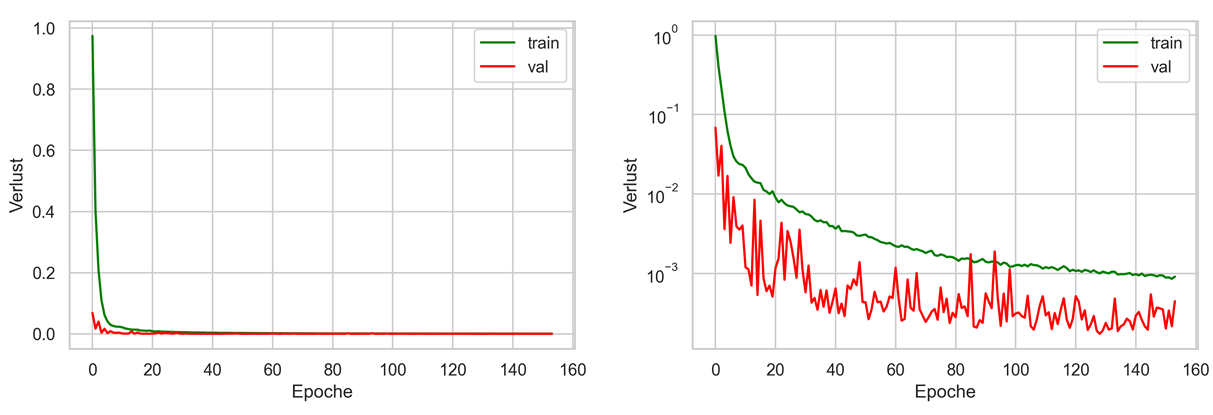
\includegraphics[width=16cm]{98_images/normal_log_vgg.png}
\caption{Verläufe des Trainingsvorgangs der VGG19-Architektur in linearer (links) und logarithmischer (rechts) Darstellung}
\label{fig:vgg-verlaeufe}
\end{figure}

\mypar Am logarithmischen Verlauf ist ebenfalls ersichtlich, dass das Netz bessere Ergebnisse in der Validierung als im Training erzielt. Dafür gibt es zwei Gründe. Zum einen wird das Dropout nicht im Validierungs- und Testvorgang angewendet, sondern nur während des Trainings. Zum anderen wird der Verlust im Training während den entsprechenden Epochen gemessen und aktualisiert. Im Gegensatz dazu wird der Validierungsfehler nach jeder Epoche berechnet, sodass die Parameter zu diesem Zeitpunkt auf angepassten Werten liegen.

\mypar Die Funktionsweise eines trainierten faltenden neuronalen Netzes kann mithilfe der Ausgaben aus den einzelnen Layern aufgezeigt werden. Ein vortrainiertes VGG19 erzeugt nach dem ersten Convolutional Layer 64 Feature Maps (siehe Abschnitt \ref{sec:vgg-sec}). Zehn die bei einer Eingabe des Bildes aus \ref{fig:30grad-cropped-img} entstandenen Feature Maps sind in Abbildung \ref{fig:activations-1} abgebildet.

\begin{figure}[h!]
\centering
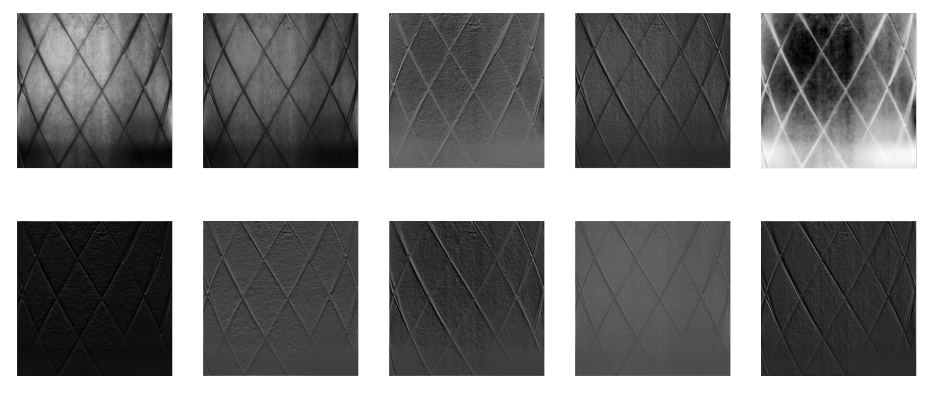
\includegraphics[width=12cm]{98_images/0_block1_conv1.png}
\caption{Zehn der 64 Feature Maps, welche durch das erste Convolutional Layer einer trainierten VGG19-Architektur entstehen}
\label{fig:activations-1}
\end{figure}

\mypar Durch die Anwendung der unterschiedlichen Filter aus dem Convolutional Layer werden die Kanten, also die Drähte des Stents, hervorgehoben. In den darauffolgenden Schritten wird die Dimensionalität der Eingabe durch die Anwendung weiterer Filter reduziert. Ebenso werden die Drähte im Bild verdeutlicht und der Hintergrund homogenisiert, wie in den Beispielen aus Abbildung \ref{fig:activations-2} gezeigt.

\begin{figure}[h!]
\centering
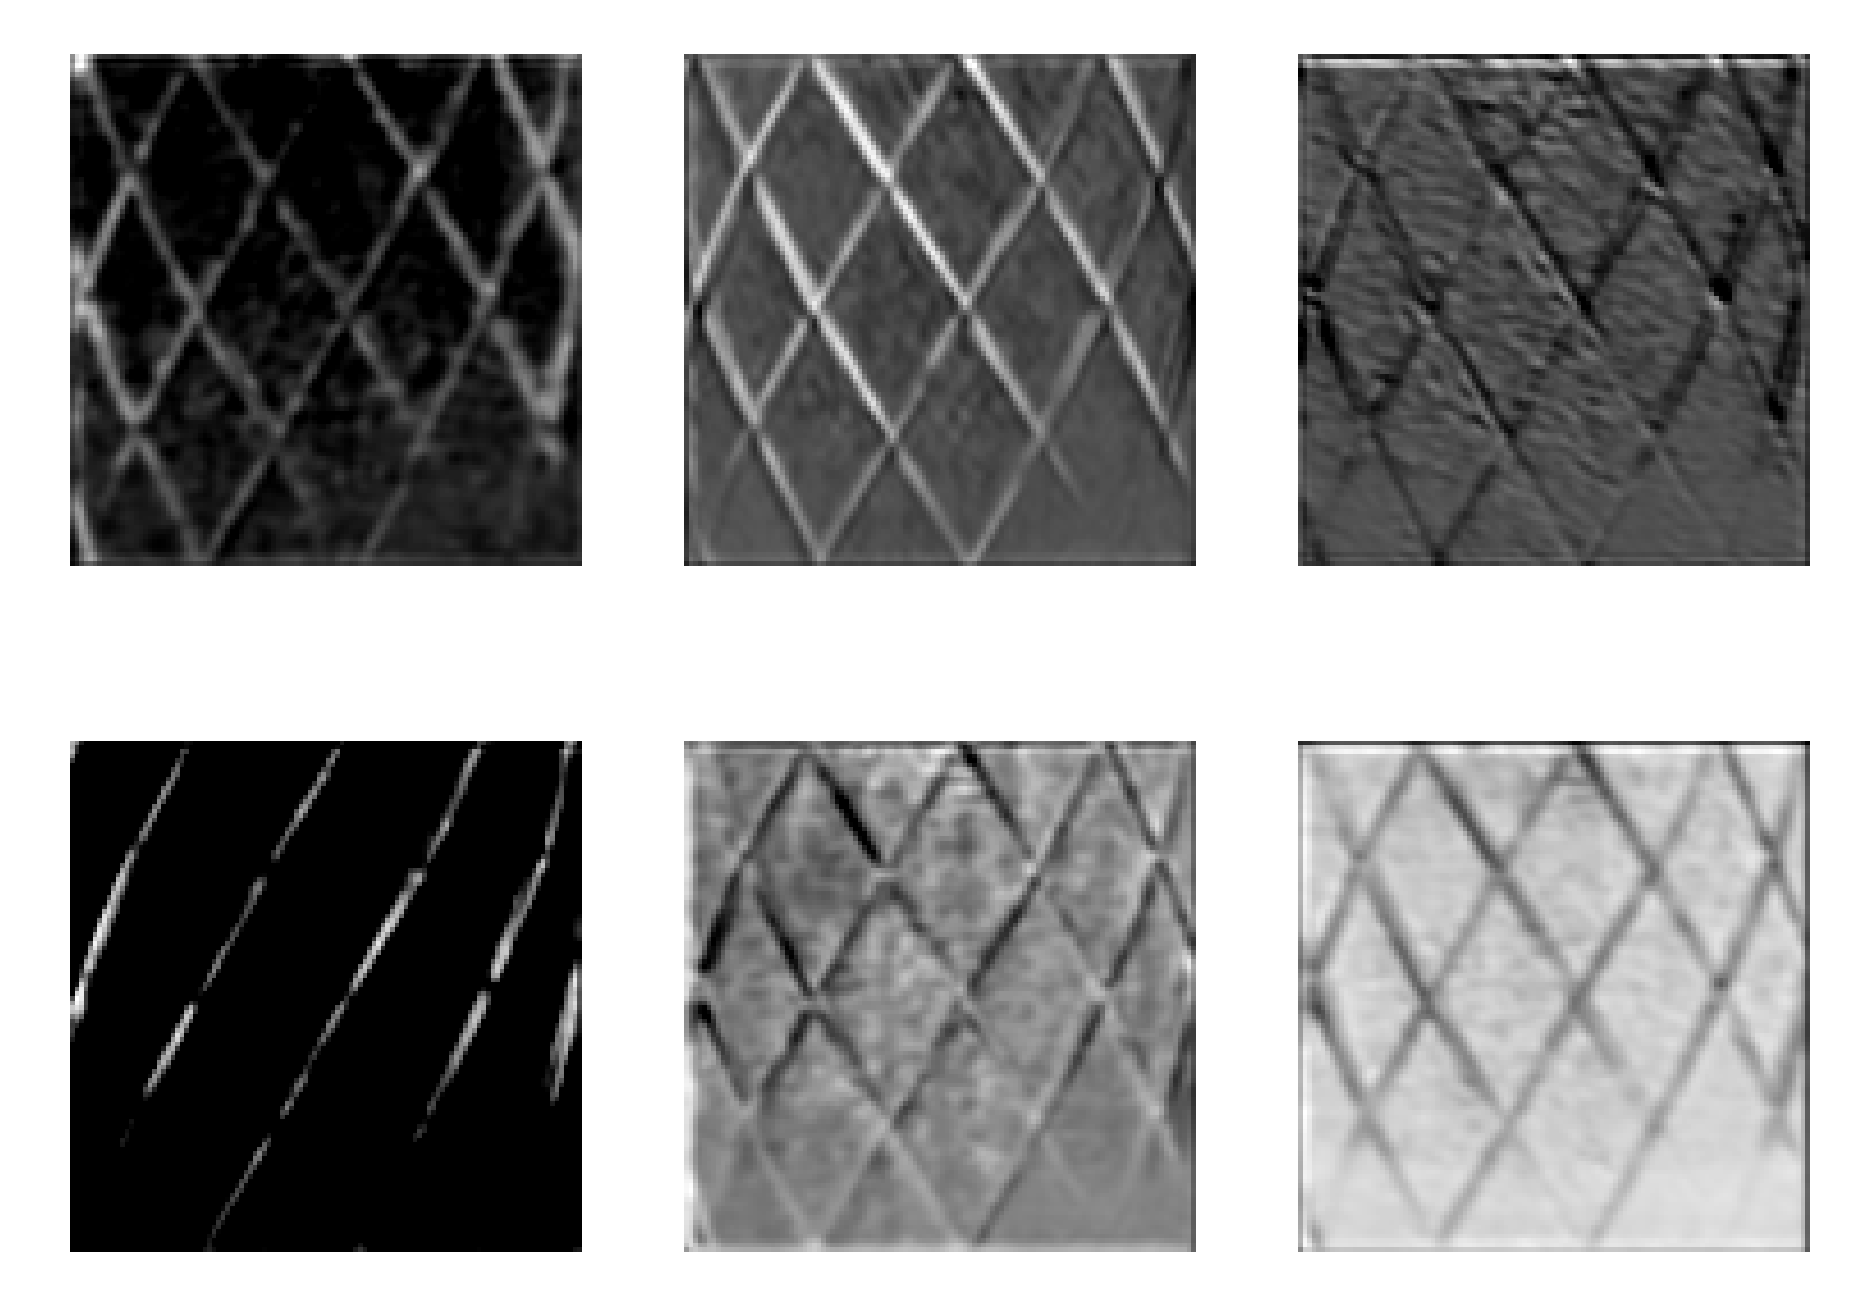
\includegraphics[width=7cm]{98_images/0_block3_conv4.png}
\caption{Sechs der 256 Feature Maps aus dem vierten und letzten Convolutional Layer im dritten Block des VGG19}
\label{fig:activations-2}
\end{figure}


% Bewertung der Ergebnisse
\section{Bewertung und Vergleich der Ergebnisse}
Insgesamt wurden drei grundlegende Vergleichsfaktoren gewählt: Der Fehler, welcher die durchschnittliche Abweichung zwischen der Netzausgabe und dem Soll-Wert darstellt, die benötigte Rechenzeit pro Bild und die gesamte Dauer des Trainings der Netze. Im Folgenden werden die Trainings- und Testergebnisse der einzelnen Netze miteinander bezüglich den zuvor genannten Faktoren verglichen. Eine Übersicht mit allen faltenden neuronalen Netzen und den Vergleichsgrößen wird in Anhang \ref{ch:Anhang-ch} in Tabelle \ref{Tab:vergleich-netze} aufgezeigt. 


% Fehler
\subsection{Fehler}\label{sec:fehler-sec}
Der Fehler ist das wichtigste Vergleichskriterium unter den neuronalen Netzen, da es sich auf die Genauigkeit dieser bezieht. Um Fehler möglichst richtig zu erkennen, muss das Netzwerk die Länge des Picks möglichst zuverlässig bestimmen können. 

\mypar Aus Abbildung \ref{fig:year-error-graph} kann abgelesen werden, dass das VGG19 in dieser Kategorie das beste Ergebnis erreicht. Die durchschnittliche Abweichung von 1,76 Pixel entpricht etwa 0,077 mm. Zudem schneidet das AlexNet, die älteste Architektur aus der Auswahl, mit Abstand am schlechtesten ab. Die neueste Architektur, das EfficientNet B2, erreicht in diesem Fall eine durchschnittliche Leistung bei 3,24 Pixel.


% Rechenzeit pro Bild
\subsection{Rechenzeit pro Bild}\label{sec:rechenzeit-label}
Als allgemeine Randbedingung wurde vorgegeben, dass das Gesamtsystem zur Fehlererkennung und -Korrektur in der Lage sein muss mindestens zehn Picks pro Sekunde zu inspizieren. Da das Bild durch alle Schichten der neuronalen Netze gespeist werden muss, hat die Anzahl an Schichten einen Einfluss auf die Dauer dieses Vorgangs. Abbildung \ref{fig:year-time-graph} zeigt die benötige Rechenzeit für ein Bild je Netz, wobei diese nach dem Veröffentlichungsjahr sortiert sind. Das AlexNet besitzt die niedrigste Anzahl an Schichten (sieben) und analysiert Bilder am schnellsten. Im Gegensatz dazu ist das Inception-ResNet-v2 das tiefste Netz und verbraucht die meiste Zeit zur Analyse. Trotz dieser Korrelation und des Einflusses der Anzahl an Schichten auf die Rechenzeit, sind beide Werte nicht proportional zueinander. Trotz der zweitniedrigsten Anzahl an Schichten verbraucht beispielsweise das VGG16 viel Zeit für die Analyse der Picklänge.

\begin{figure}[h!]
\centering
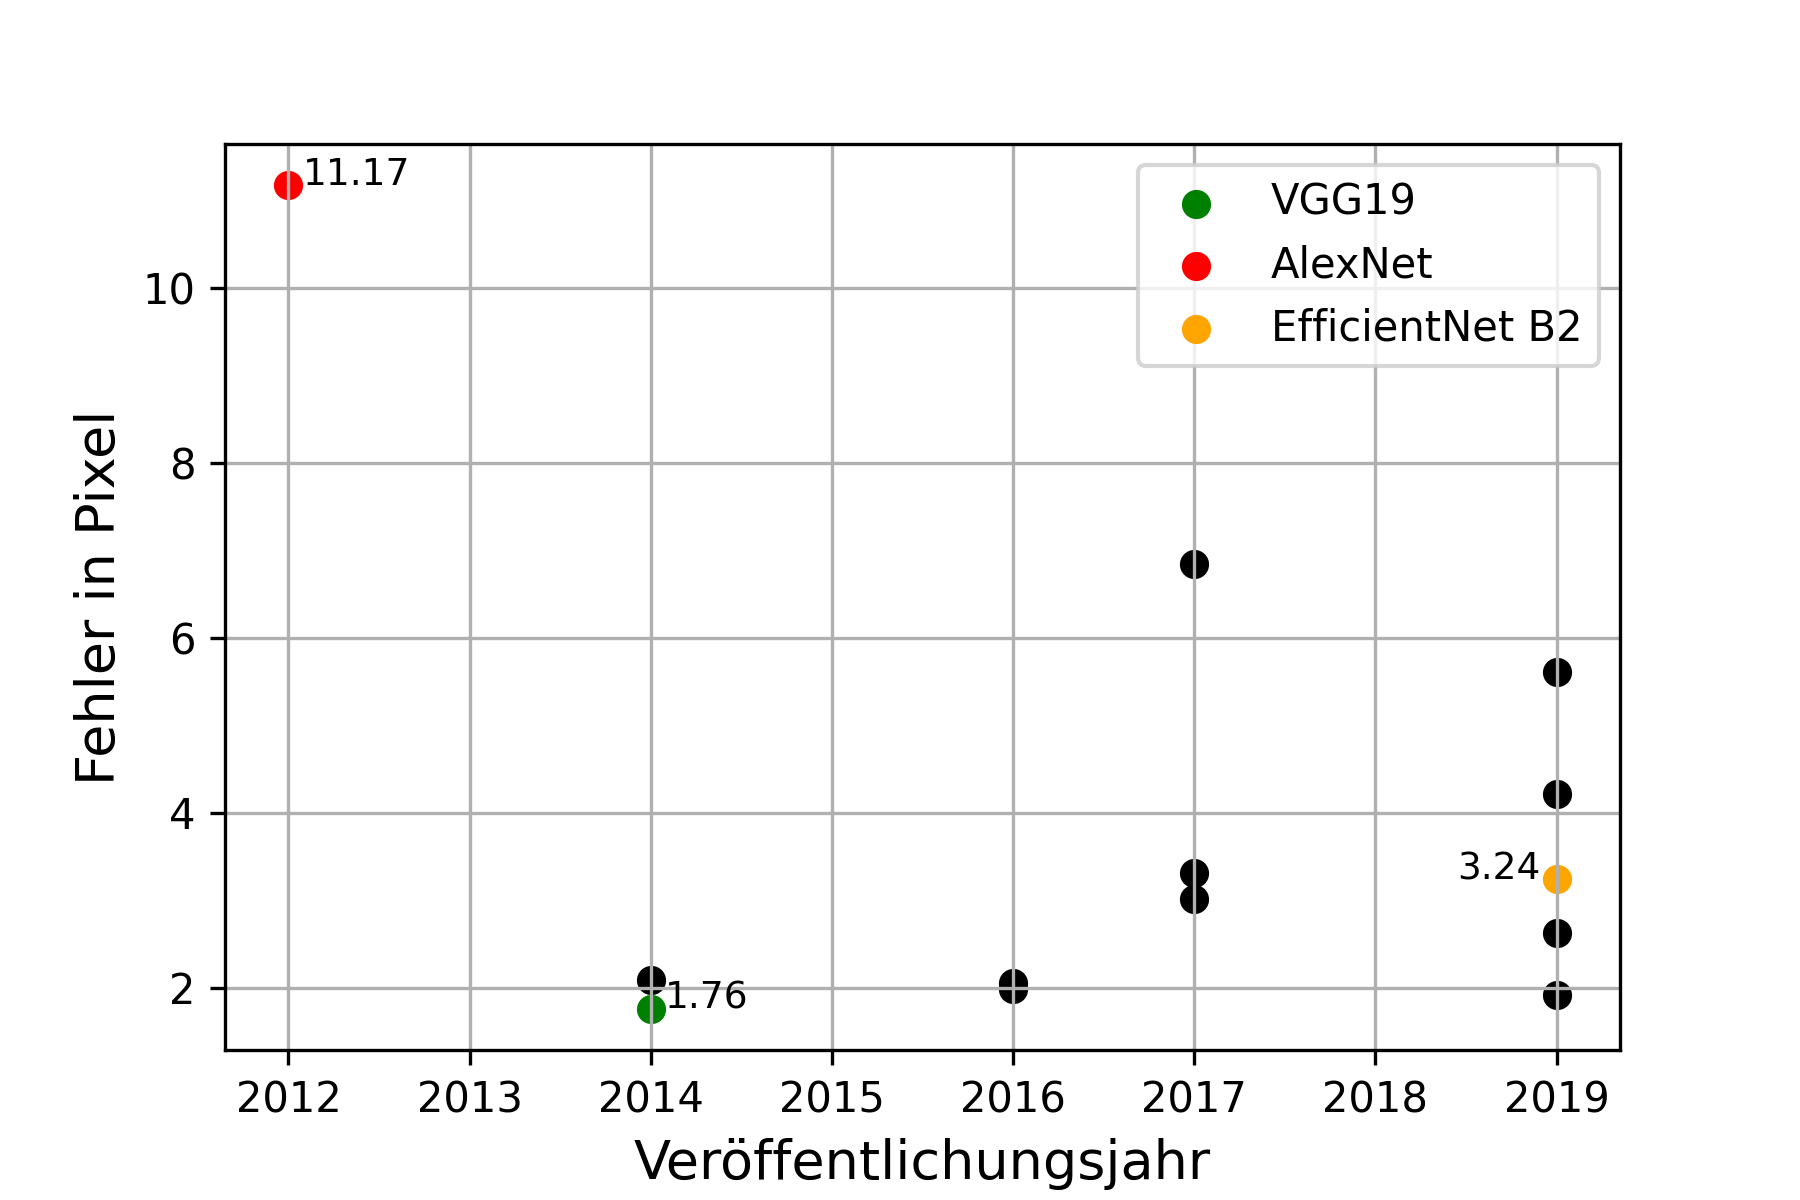
\includegraphics[width=11cm]{98_images/year_error_graph.png}
\caption{Vergleich des Fehlers nach Veröffentlichungsjahr der Netzwerkarchitekturen}
\label{fig:year-error-graph}
\end{figure}

\begin{figure}[h!]
\centering
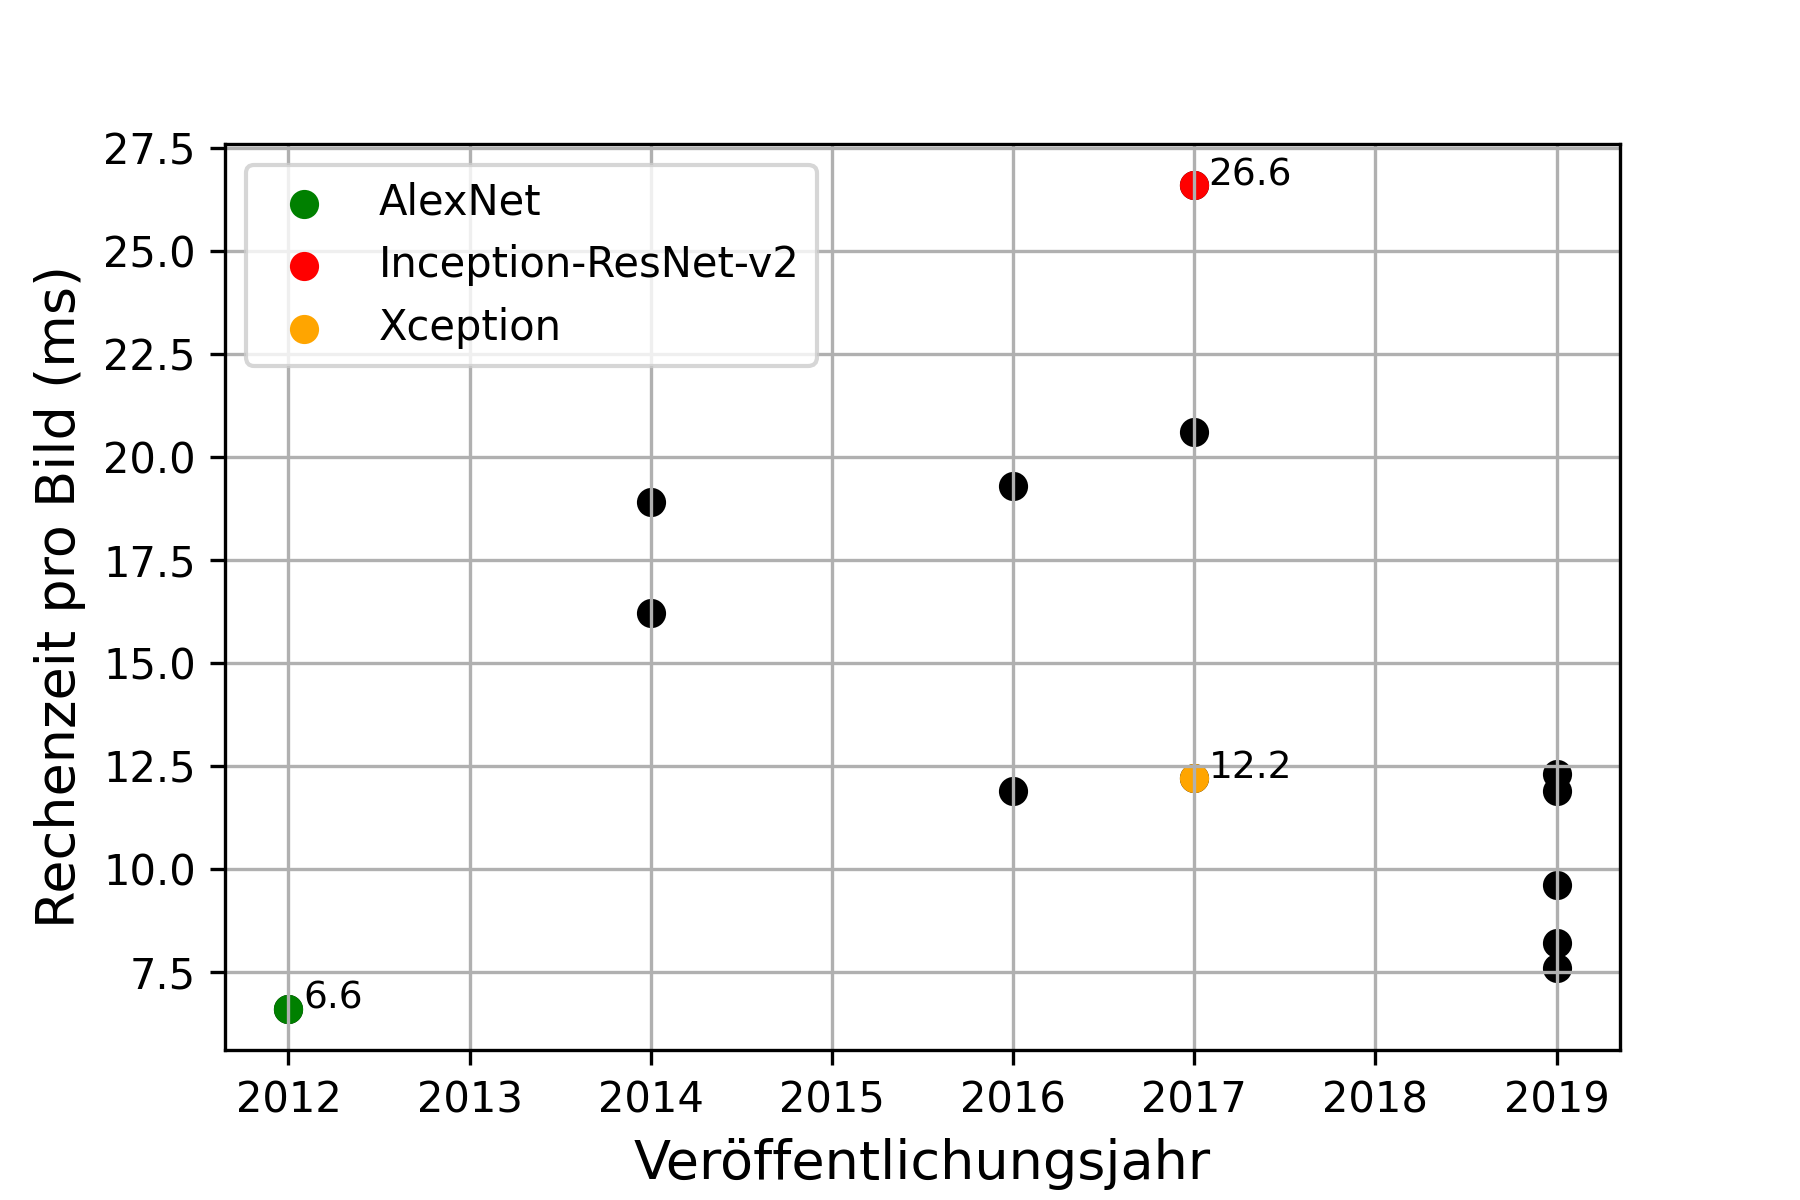
\includegraphics[width=11cm]{98_images/year_time_graph.png}
\caption{Vergleich der Rechenzeit pro Bild nach Veröffentlichungsjahr der Netzwerkarchitekturen}
\label{fig:year-time-graph}
\end{figure}

\mypar Nach Angaben des Industriepartners muss das Gesamtsystem zur Fehlererkennung und -korrektur in der Lage sein, zehn Picks innerhalb einer Sekunde zu inspizieren. Obwohl alle in diesem Abschnitt vorgestellten Werte unter dieser Schranke liegen, muss betrachtet werden, dass dies das Erfassen von Bildern, deren Vorverarbeitung, die Lokalisierung von Picks und weitere Schritte des Verfahrens nicht miteinbezieht.


% Trainingsdauer
\subsection{Trainingsdauer}
Der dritte und letzte Vergleichsfaktor unter den Netzen ist die benötigte Trainingsdauer. Allerdings hat diese keinen Einfluss auf die Leistung der neuronalen Netzwerke. Aufgrund seiner geringen Anzahl an Schichten schneidet hier die AlexNet-Architektur am besten ab. Unter den restlichen Modellen schwankt die Trainingsdauer zwischen zehn und zwanzig Stunden. Eine Übersicht der beim Fehler und Rechenzeit hervorgehobenen Netze, aus den Abschnitten \ref{sec:fehler-sec} und \ref{sec:rechenzeit-label}, ist in Tabelle \ref{Tab:vergleich-netze} aufgezeigt.


% Fehler zu Rechenzeit
\subsection{Fehler zu Rechenzeit}
Da der Fehler und die Rechenzeit die wichtigsten Faktoren sind, wurden diese ebenfalls, wie in Abbildung \ref{fig:time_error_graph} zu sehen, miteinander verglichen. Anhand des Graphens ist ersichtlich, dass das VGG19 zwar den niedrigsten Fehler macht, sich dennoch unter den langsamsten Netzen bei der Vermessung der Picklänge befindet. Im Gegensatz dazu führt das MobileNetV3 large zu einer leicht höheren durchschnittlichen Abweichung von etwa 0,16 Pixel. Dafür wird die Länge eines Picks mehr als doppelt so schnell wie beim VGG19 vermessen. Bei der small Variante der MobileNetV3-Architektur beträgt diese Zeit etwas weniger als bei der large Variante. Allerdings ist der Unterschied beim erzeugten Fehler im Vergleich zum MobileNetV3 large deutlich größer. 

\begin{figure}[h!]
\centering
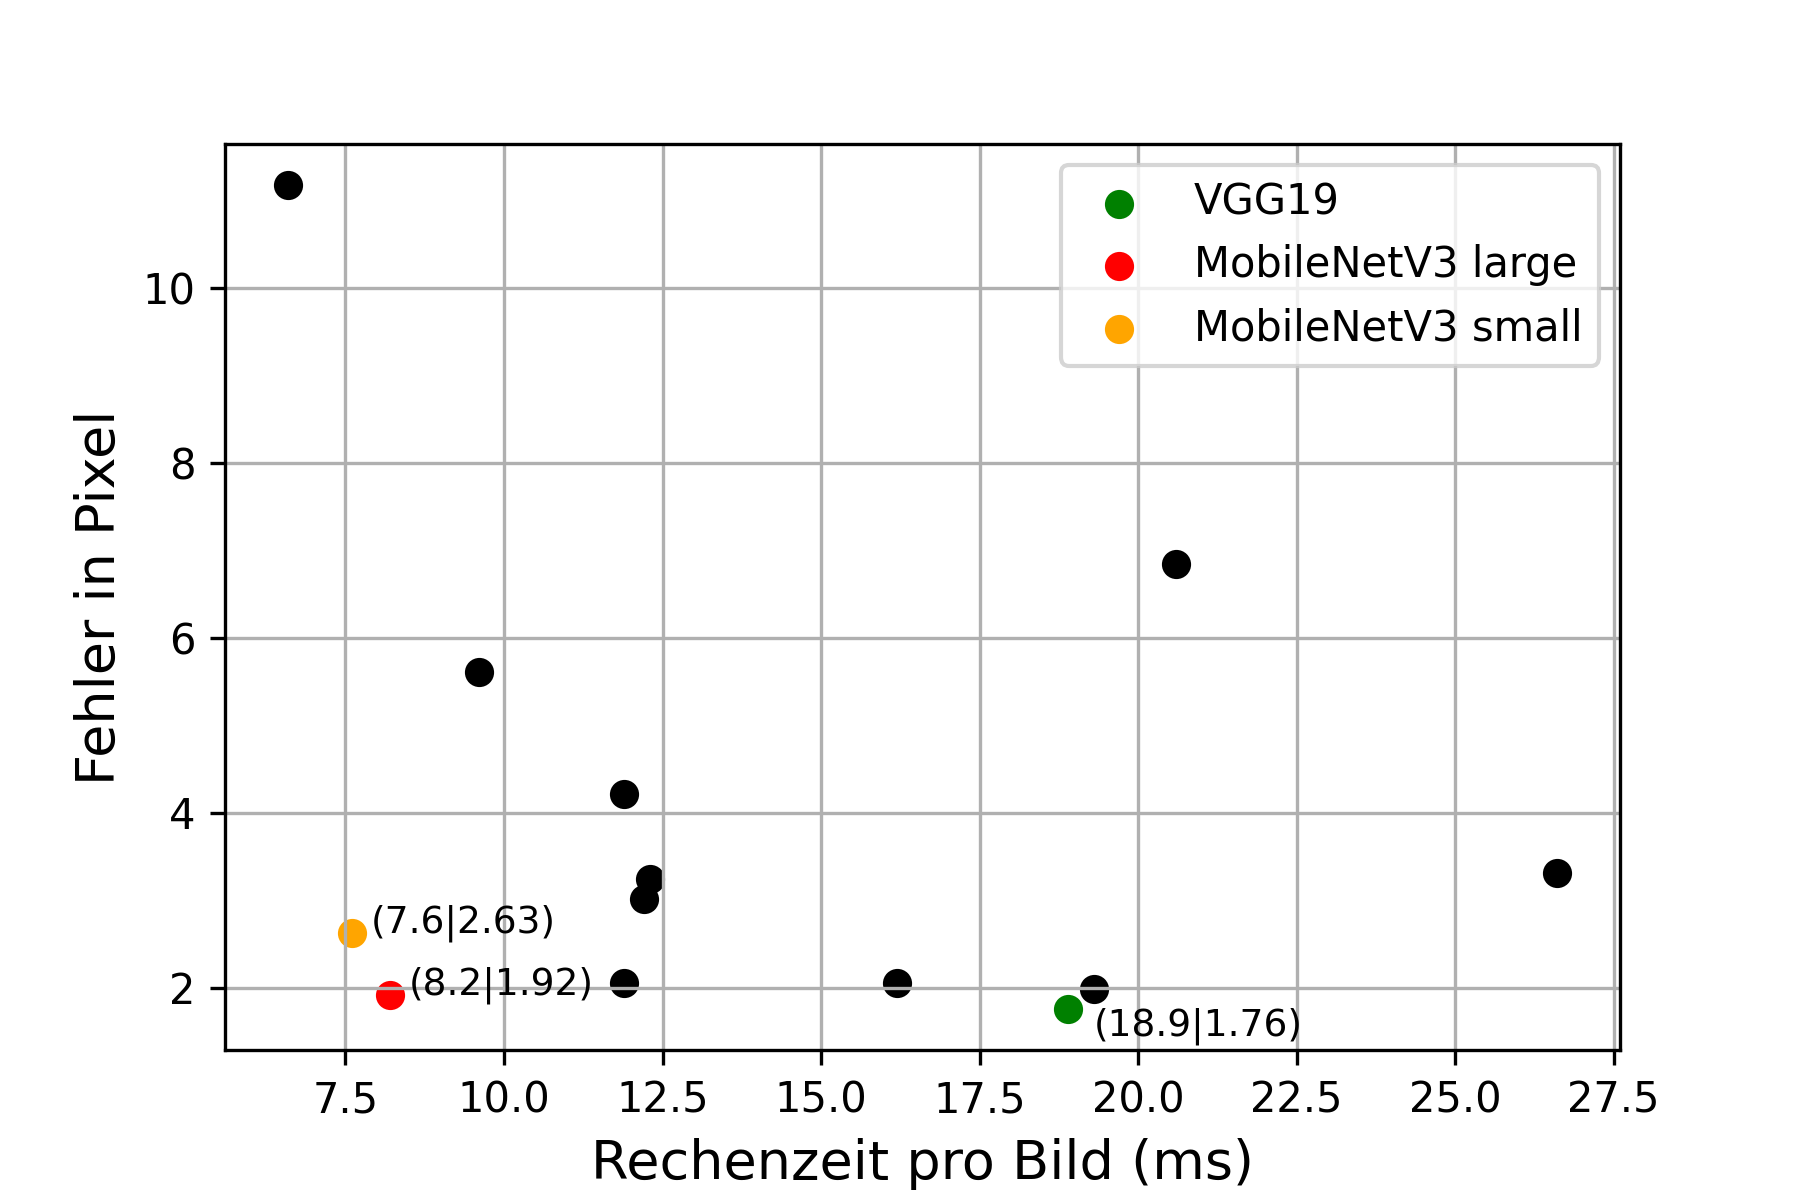
\includegraphics[width=11cm]{98_images/time_error_graph.png}
\caption{Vergleich des Fehlers nach der benötigten Rechenzeit pro Bild}
\label{fig:time_error_graph}
\end{figure}


% Bestimmung der Abweichung
\section{Bestimmung der Abweichung}
Zu Beginn des Flechtvorgangs sind sowohl der Soll-Wert $l_{soll}$ für die Länge der Picks, als auch ein beliebiger Toleranzwert $l_t$ angegeben. Darauffolgend wird, aus der Analyse eines Picks durch ein faltendes neuronales Netz, die vom System gemessene Picklänge ausgegeben, welche dem Ist-Wert $l_{ist}$ entspricht. Somit kann die Abweichung $l_{diff}$ der Netzausgabe durch den Betrag der Differenz zwischen dem Soll- und Ist-Wert wie in Gleichung \ref{eq:abweichung-netz} berechnet werden. 

\begin{equation}\label{eq:abweichung-netz}
l_{diff} = | l_{soll}-l_{ist} |
\end{equation}

\mypar Die Werte der Abweichungen eines Netzes können als Histogramm dargestellt werden. Ein solches Diagramm ist in Abbildung \ref{fig:vgg-histogramm} für das Testen einer trainierten VGG19-Architektur auf den Testdatensatz abgebildet. Für die meisten Bilder beträgt die Abweichung der Netzausgaben weniger als einen Pixel. Da es bei allen Netzen oftmals zu Ausgaben kommt, welche eine große Differenz aufweisen, wurde dies in Abschnitt \ref{sec:fehlerquellen-sec} näher untersucht.

\begin{figure}[h!]
\centering
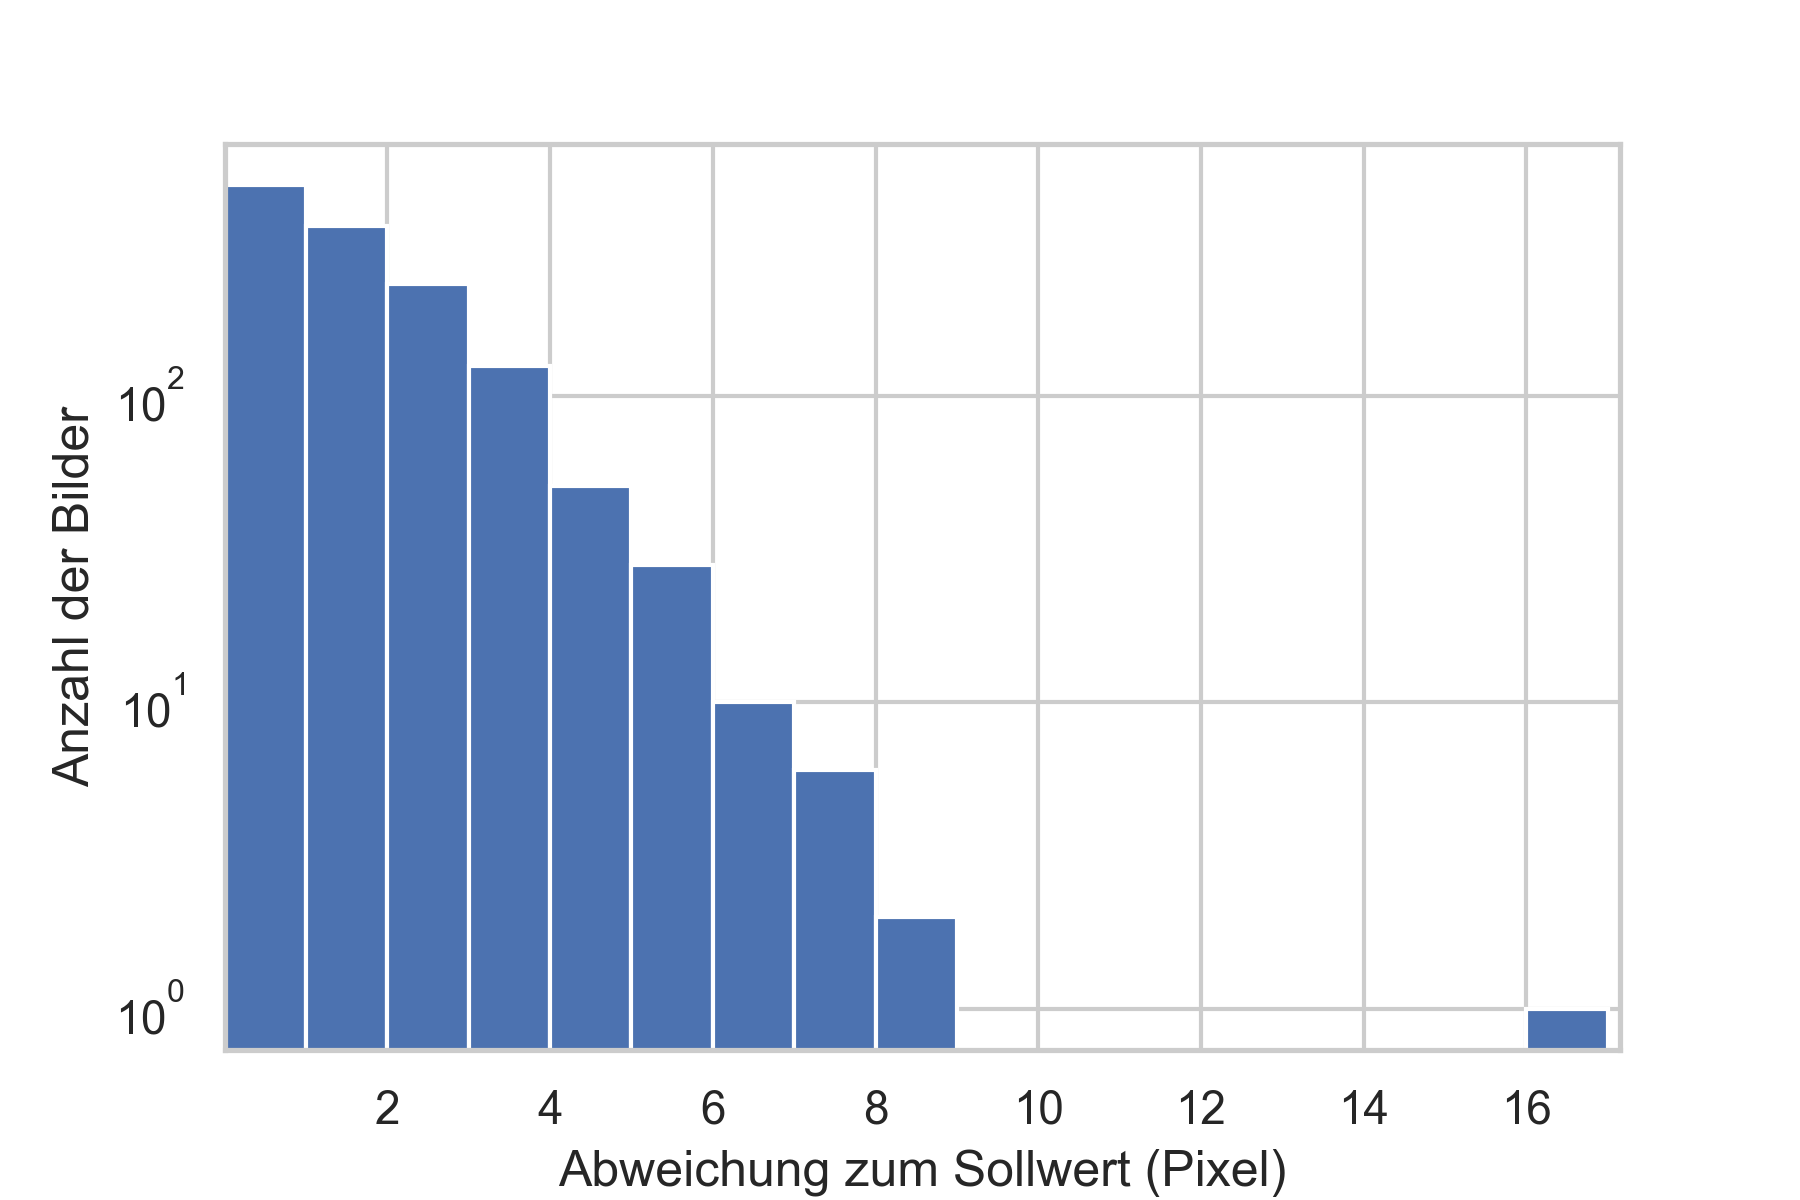
\includegraphics[width=10cm]{98_images/vgg_histogramm.png}
\caption{Aufteilung der Abweichungen bei den Ausgaben eines trainierten VGG19 auf den Testdatensatz}
\label{fig:vgg-histogramm}
\end{figure}

\mypar Werden die Abweichungen der fünf Architekturen mit dem besten Fehler näher betrachtet, wie in Abbildung \ref{fig:best-worst-preds} aufgezeigt, fällt auf, dass ein besserer Fehler nicht mit einem niedrigeren Intervall zwischen der besten und schlechtesten Vermessung zusammenhängt. So liegen sowohl die größten, als auch die niedrigsten Abweichungen beim ResNet101V2 und VGG16 niedriger als bei neuronalen Netzen wie das VGG19 und MobileNetV3 large, welche einen besseren Fehler erzielen. 

\begin{figure}[h!]
\centering
\includegraphics[width=14.5cm]{98_images/best_worst_preds.png}
\caption{Aufteilung der Abweichungen unter den fünf Netzen mit dem besten Fehler}
\label{fig:best-worst-preds}
\end{figure}


% Fehlererkennung
\section{Fehlererkennung}
Die errechnete Abweichung kann mit dem Toleranzwert verglichen werden, um über einen potentiellen Defekt im Stent zu entscheiden. Sollte diese kleiner oder gleich dem Wert der Toleranz $l_t$ wie in Gleichung \ref{eq:abweichung-netz-toleranz} sein, liegt diese noch im Toleranzbereich, sodass der Pick den Qualitätsanforderungen entspricht. Andernfalls entspricht die vom Netz gemessene Picklänge nicht den vorgegebenen Anforderungen, sodass der Pick als fehlerhaft empfunden wird.

\begin{equation}\label{eq:abweichung-netz-toleranz}
l_{diff} \leq l_t
\end{equation}

\mypar Je nachdem wie der Toleranzwert festgelegt wird, wird die Leistung des Systems beeinflusst. Ist dieser zu hoch, werden weniger Defekte gemeldet, wodurch das System weniger falsch negative Ergebnisse anzeigt und die Produktivität gesteigert wird. Auf der anderen Seite können Defekte dadurch übersehen werden, womit die Genauigkeit und Zuverlässigkeit der Überprüfung sinkt. 


% Mögliche Fehlerquellen
\section{Mögliche Fehlerquellen}\label{sec:fehlerquellen-sec}
Im Rahmen dieses Abschnitts sollen Gründe für Abweichungen zwischen den Soll- und Ist-Werten erklärt werden. Für Abweichungen einer hohen Größenordnung wurden zwei Gründe festgestellt. Zum einen sind Teile des mittleren Picks auf einigen Bildern schlecht erkennbar. Im betrachteten Pick aus Abbildung \ref{fig:bilder-abweichungen} links, ist die obere Ecke der Struktur schlecht erkennbar. Aus diesem Bild ergab sich die größte Abweichung mit dem VGG19, nämlich 16,2 Pixel.

\begin{figure}[h!]
\centering
\includegraphics[width=9cm]{98_images/grosse_abweichungen.png}
\caption{Beispiele für Bilder, welche zu großen Abweichungen bei der Netzausgabe geführt haben. Der Mittelpunkt der Bilder ist rot markiert.}
\label{fig:bilder-abweichungen}
\end{figure}

\mypar Der zweite und meist verbreitete Grund ist rechts in Abbildung \ref{fig:bilder-abweichungen} dargestellt. Ein zwischen zwei Picks positionierter Mittelpunkt des Bildes führte oftmals zu großen Abweichungen bei den Netzen.

\mypar Abweichungen einer geringen Größe können aufgrund ungenauer Labels entstehen. In Anbetracht der breiten Anzahl an Bildern, von denen die Labels in Zusammenarbeit erstellt wurden, und dem unvermeidbaren menschlichen Fehler, sind Ungenauigkeiten in den Labels unumgänglich. Somit ist es möglich, dass die Netze zwar die richtigen Eigenschaften der Bilder erlernen, sich aber Abweichungen infolge ungenauer Labels bilden. 


% Bewertung des Systems
\section{Bewertung des Systems}\label{sec:bewertung-system-sec}
Bezogen auf das Projekt Stents4Tomorrow \cite{flechtmaschine} sind drei wichtige Größen für die Genauigkeit des Systems zur automatisierten Korrektur von Fehlern in Stents vorgegeben. Ein optimales System muss in der Lage sein, Picklängen mit einer Genauigkeit von $\pm 0,01$ Millimeter zu berechnen. Bei einer guten Leistung verdoppelt sich dieser Wert und ein ausreichendes Ergebnis bedingt eine Genauigkeit von 0,05 Millimeter. Diese Werte werden als $l_1$, $l_2$ und $l_3$ gekennzeichnet.

\mypar Abbildung \ref{fig:abweichungen-je-toleranz} zeigt den prozentualen Anteil an Bildern aus dem Testdatensatz, welche von unterschiedlichen Netzen bei einen gewissen Toleranzwert richtig vermessen werden. Hierbei sind die drei zuvor erläuterten Vorgaben ebenso im Graphen eingetragen. Hieraus kann abgelesen werden, dass die zwei Netze mit dem besten Fehler, das VGG19 und MobileNetV3, ab einer Toleranz von etwa sieben Pixeln nahe an die 100{\%} kommen. Die aus der Auswahl neueste Architektur, das EfficientNet B2, benötigt etwa 11,5 Pixel. Das AlexNet hingegen erreicht, trotz einer Toleranz von 12 Pixeln, was mehr als einen halben Millimeter entspricht, eine Genauigkeit von ungefähr 65{\%}.

\begin{figure}[h!]
\centering
\includegraphics[width=14cm]{98_images/abweichungen_nach_toleranz.png}
\caption{Prozentanteil der Ausgaben mehrerer Netze je nach gesetzter Toleranz. Die drei vorgegebenen Größen $l_1 = 0,23 \text{ Pixel}, l_2 = 0,46 \text{ Pixel und } l_3 = 1,15 \text{ Pixel}$ sind eingezeichnet.}
\label{fig:abweichungen-je-toleranz}
\end{figure}

\mypar Werden diese Ergebnisse nun mit den Zielwerten verglichen, wird deutlich, dass die $l_1$- und $l_2$-Werte aktuell noch nicht erreicht werden können. Die Ak­ku­ra­tes­se des aktuell genauesten Netzes liegt hinsichtlich dieser Werte bei etwa 8,1{\%} und 16,8{\%}. Selbst eine ausreichend gute Vermessung der Picklänge kann aktuell nur in ungefähr 43,3{\%} der Fälle erreicht werden.




    \cleardoublepage    

    \chapter{Fazit und Ausblick}
    \label{ch:Fazit}    
    	In dieser Arbeit wurden neun Architekturen und einige ihrer Varianten, also dreizehn faltende neuronale Netze bezüglich einer Regression der Picklänge kardiovaskulärer Implantate untersucht. Hierfür wurden zur Verfügung gestellte Daten vorverarbeitet und augmentiert. Darauffolgend wurden die einzelnen neuronalen Netze implementiert, angepasst, trainiert und daraufhin evaluiert. Basierend auf den Evaluationsergebnissen, wurden die Netze hinsichtlich einer Regression der Picklänge der Implantate miteinander verglichen. 

\mypar Aus der Bewertung der neuronalen Netze und dem anschließenden Vergleich hat das VGG19 die besten Ergebnisse in Bezug auf die durchschnittliche Abweichung erzielt. Diese beträgt 1,76 Pixel oder 0,077 Millimeter, sodass der Fehler bei der kleinsten und der größten Picklänge des Datensatzes 4,4 {\%} bzw. 0,8 {\%} beträgt. Überdies beträgt der Fehler des MobileNetV3 large 0,16 Pixel mehr, doch die erforderliche Rechenzeit, um die Länge eines Picks zu berechnen, wird mehr als halbiert. Hinsichtlich einer zuverlässigen und zugleich zeitlich effizienten Überprüfung der Stentgeometrie kann dieser Faktor im weiteren Verlauf des Projekts von großer Bedeutung sein.

\mypar Die in Abschnitt \ref{sec:bewertung-system-sec} erläuterten Zielanforderungen an das System sind unter den aktuellen Umständen nicht erfüllbar. Gründe dafür sind der menschliche Fehler bei der Erstellung der Labels für die Bilddaten, die verfügbare Rechenleistung und die Auflösung der aktuellen zugeschnittenen Aufnahmen.

\mypar Im nächsten Schritt des Projektes ist die Durchführung einer Hyperparameteroptimierung mit den besten faltenden neuronalen Netzen sinnvoll. Daraus können die Ergebnisse dieser Arbeit weiterhin verbessert werden. Aufgrund des verfügbaren Rechners und der begrenzten Zeit für dessen Verwendung war eine solche Optimierung der Hyperparameter nicht möglich.

\mypar Außerdem kann der Datensatz mit weiteren Flechtwinkeln erweitert und diversifiziert werden, da dieser aktuell aus Bildern mit nur fünf unterschiedlichen Flechtwinkeln besteht. Dadurch bilden sich unter den Ausgaben der trainierten Netzwerkarchitekturen fünf unterschiedliche Cluster.

\mypar Zudem können Bilder mit unterschiedlichen Lichtverhältnissen und Hintergründen hinzugefügt werden, um die Fähigkeit der Generalisierung von den neuronalen Netzen zu steigern und somit deren Leistung zu verbessern, sodass die Längen der einzelnen Picks genauer und zuverlässiger bestimmt werden können. Für die Umsetzung der angesetzten Ideen bezüglich des Datensatzes kann die Erzeugung künstlicher Bilddaten inklusive Labels untersucht werden. Zu diesem Zweck können beispielsweise Generative Adversarial Networks \cite{goodfellow2014generative}, Generative Teaching Networks \cite{such2020generative} oder weitere Verfahren erprobt werden.
    \cleardoublepage
    
% =====================================================
% Bibliography
% ===================================================== 
% \nocite{*}
%\addcontentsline{toc}{chapter}{Literaturverzeichnis, in ToC löschen}
%\addcontentsline{toc}{chapter}{Literature}
%\bibliographystyle{dinat}        % use a DIN style for the bibliography
%\bibliographystyle{plain}        % use a DIN style for the bibliography
%\bibliographystyle{abbrv}			%mit nummern in []
%\bibliographystyle{plain}			%mit nummern in []
%\bibliographystyle{alpha}			%3 Buchstaben + Jahr
%\bibliographystyle{alphadin}		%Nachname(n) + Jahr
\bibliographystyle{alphadin}

    % use external Bib-File, 
		\bibliography{99_bib/standardbib}		
		\cleardoublepage
% =====================================================
% Appendix
% ===================================================== 
    \appendix
    
    \chapter{Anhang}
    \label{ch:Anhang-ch}
    	\begin{table}[ht]
\begin{center}
\begin{tabular}{l|c|c|c}
\textbf{Architektur} & \textbf{Fehler (Pixel)} & \textbf{Rechenzeit (ms)} & \textbf{Trainingsdauer} \\ \hline
VGG19                & 1,764                   & 18,9                     & 15h 48m 28s             \\ \hline
MobileNetV3 large    & 1,924                   & 8,2                      & 14h 5m 24s              \\ \hline
ResNet101V2          & 1,988                   & 19,3                     & 18h 15m 18s             \\ \hline
ResNet50V2           & 2,045                   & 11,9                     & 13h 24m 31s             \\ \hline
VGG16                & 2,085                   & 16,2                     & 8h 40m 55s              \\ \hline
MobileNetV3 small    & 2,634                   & 7,6                      & 22h 4m 32s              \\ \hline
Xception             & 3,020                   & 12,2                     & 12h 30m 33s             \\ \hline
EfficientNet B2      & 3,242                   & 12,3                     & 16h 56m 49s             \\ \hline
Inception-ResNet-v2  & 3,311                   & 26,6                     & 20h 32m 46s             \\ \hline
EfficientNet B1      & 4,206                   & 11,9                     & 10h 52m 11s             \\ \hline
EfficientNet B0      & 5,612                   & 9,6                      & 7h 26m 50s              \\ \hline
Inception-v4         & 6,840                   & 20,6                     & 12h 7m 27s              \\ \hline
AlexNet              & 11,167                  & 6,6                      & 4h 55m 54s             
\end{tabular}
\caption{Vergleich der Trainings- und Testergebnisse aller Architekturen. Betrachtet wird der Fehler, welcher die durchschnittliche Abweichung zwischen der Netzausgabe und dem Soll-Wert darstellt, die Rechenzeit pro Bild und die gesamte Trainingsdauer der einzelnen Netze.}
\label{Tab:vergleich-netze}
\end{center}
\end{table}
		\cleardoublepage

    \listoftables
    	\cleardoublepage
    \listoffigures
    	\cleardoublepage
    \printindex
    	\cleardoublepage
    \printnomenclature
    \renewcommand{\leftmark}{\uppercase{Abkürzungsverzeichnis}}
    	\cleardoublepage

\end{document}

